\documentclass[letterpaper, 10pt, conference]{IEEEtran}
\usepackage{amsmath,amssymb}
\usepackage{graphicx}
\usepackage{booktabs}
\usepackage{multirow}
\usepackage{array}
\usepackage{float}
\usepackage[colorlinks=true,
            linkcolor=blue!60!black,
            citecolor=blue!60!black,
            urlcolor=blue!60!black,
            bookmarksnumbered=true,
            pdftitle={A Ball-on-Arc Benchmark: Classical and Learning-Based Control on Realistic Deployment Hardware (Supplementary Material)},
            pdfauthor={Jaydeepkumar Ranpariya; Sandipan Nath; Alexander Mattick; Georgios Kontes; Tobias Feigl; Christopher Mutschler},
            pdfsubject={Supplementary material for an arXiv preprint}]{hyperref}
\usepackage{xcolor}
\usepackage{tikz}
\usetikzlibrary{arrows.meta, positioning, fit, backgrounds, calc}
\usepackage{caption}
% Arabic table numbers: with 30+ tables, Roman numerals reach "Table XXX",
% which reads like an unfilled placeholder. Arabic (Table 30) is clearer.
\renewcommand{\thetable}{\arabic{table}}
% IEEE-style figure/table captions: small bold label, ragged-right, tight spacing
\captionsetup{font=small, labelfont=bf, labelsep=period,
              justification=raggedright, singlelinecheck=false,
              aboveskip=4pt, belowskip=2pt}
\usepackage{listings}
\lstset{basicstyle=\ttfamily\small,breaklines=true,frame=single,
  backgroundcolor=\color{gray!8},xleftmargin=1em,xrightmargin=1em,
  aboveskip=4pt,belowskip=4pt}

\title{A Ball-on-Arc Benchmark: Classical and Learning-Based Control on Realistic Deployment Hardware\\\Large Supplementary Material}
\author{
Jaydeepkumar Ranpariya, Sandipan Nath, Alexander Mattick, Georgios Kontes, Tobias Feigl, and Christopher Mutschler\\
Fraunhofer Institute for Integrated Circuits IIS, Nuremberg, Germany}

\begin{document}
\maketitle

\begin{abstract}
This document provides supplementary technical details for the main paper
``A Ball-on-Arc Benchmark: Classical and Learning-Based Control on Realistic Deployment Hardware,'' organized into five parts.
\emph{Part~I (System)} covers (I)~sensor characterization and calibration
and (II)~the mathematical model of the plant.
\emph{Part~II (Controller Implementation)} covers (III)~controller design,
(IV)~classical controller tuning insights and failure modes,
(V)~reinforcement learning training details including PPO ablation,
multi-algorithm comparison, blind-zone ablation, motor-model ablation,
offline RL, and sim-to-real transfer, (VI)~world-model RL training, and
(VII)~MPPI controller tuning.
\emph{Part~III (Experimental Setup)} covers (VIII)~the dataset collection
protocol and (IX)~the evaluation protocol.
\emph{Part~IV (Results and Discussion)} covers (X)~simulation validation
of the analytical and learned dynamics models via open-loop prediction
accuracy, (XI)~detailed statistics and per-trial data, (XII)~results,
analysis, and discussion, and (XIII)~real-hardware fine-tuning.
\emph{Part~V} is (XIV)~the reproducibility guide.
\end{abstract}

\tableofcontents
\newpage

% Sections flow continuously (no forced per-section page breaks); the only
% \clearpage is before the bibliography, to flush any pending floats.
% ------------------------------------------------------------
% PART I - System
% ------------------------------------------------------------
\section{Sensor Characterization}
\label{appendix:sensor_characterization}


\subsection{VL53L0X Time-of-Flight Sensor}

The position sensor is one of the defining sources of difficulty on this
platform, so we characterize its behavior carefully before turning to the
controllers. Ball position is read by two VL53L0X (STMicroelectronics)
Time-of-Flight sensors, each with a programmable timing budget that sets the
integration time per measurement. We mount one at each end of the nearly
30\,cm arc (radius 2.101\,m, approximately linear) so that whichever half of
the arc the ball occupies is always read by the nearer sensor: the left sensor
covers the left half, the right sensor the right half. This nominal span
corresponds to $\pm 0.071$\,rad at $R = 2.101$\,m; logged ball angles
occasionally reach the $\pm 0.081$\,rad empirical limit used elsewhere,
because each sensor's 0--170\,mm range can report the ball marginally past the
nominal arc ends. Both share a single I$^2$C bus,
which precludes reading them simultaneously without interference.

\subsection{Sequential Mode}

In sequential mode we trigger and read the two sensors alternately. The
total cycle time we measure follows
$T_\text{cycle} \approx 2\times\text{budget} + 12\,\text{ms}$,
where the $\sim$12\,ms overhead comes from the I$^2$C transactions and the
inter-trigger delay. To map the tradeoff between noise and update rate, we
held the ball static at three positions, the center of the arc and each
extreme, and averaged 50 samples per position at four timing budgets
(Table~\ref{tab:seq_char}). The minimum programmable budget is 20\,ms, which
caps the sequential update rate at ${\approx}18.6$\,Hz.

\begin{table*}[!t]
\centering
\caption{VL53L0X sequential mode characterization. All values are
         mean\,$\pm\,\sigma$ (mm), averaged over 50 static measurements.
         $^\dagger$Interpolated by applying the $\sigma$ scaling factor
         observed across measured entries; means are physically stable.}
\label{tab:seq_char}
\resizebox{\textwidth}{!}{%
\begin{tabular}{ccc cc cc cc}
\toprule
\multirow{2}{*}{\shortstack{\textbf{Budget}\\(ms)}}
  & \multirow{2}{*}{\shortstack{\textbf{Cycle}\\(ms)}}
  & \multirow{2}{*}{\shortstack{\textbf{Rate}\\(Hz)}}
  & \multicolumn{2}{c}{\textbf{Center}}
  & \multicolumn{2}{c}{\textbf{Left Extreme}}
  & \multicolumn{2}{c}{\textbf{Right Extreme}} \\
\cmidrule(lr){4-5}\cmidrule(lr){6-7}\cmidrule(lr){8-9}
 & & & $L$ & $R$ & $L_\text{min}$ & $R_\text{max}$
       & $L_\text{max}$ & $R_\text{min}$ \\
\midrule
100  & 211.7 & 4.72  
  & $161.80\pm0.85$ & $175.76\pm1.06$
  & $48.32\pm0.99$         & $210.46\pm1.01$
  & $181.22\pm0.97$        & $40.32\pm1.00$ \\
50   & 113.2 & 8.84  
  & $161.34\pm1.24$ & $175.46\pm1.51$
  & $48.20\pm1.44^\dagger$ & $210.30\pm1.47^\dagger$
  & $180.68\pm1.54$        & $40.58\pm1.14$ \\
34.5 & 82.1  & 12.17 
  & $160.54\pm1.62$ & $175.64\pm1.68$
  & $48.08\pm1.90^\dagger$ & $210.12\pm1.93^\dagger$
  & $180.44\pm2.11$        & $41.62\pm1.78$ \\
20   & 53.8  & 18.59 
  & $160.22\pm2.83$ & $176.42\pm2.81$
  & $47.78\pm3.29^\dagger$ & $209.74\pm3.36^\dagger$
  & $180.12\pm3.22$        & $42.34\pm3.01$ \\
\bottomrule
\end{tabular}%
}
\end{table*}

Two systematic effects appear consistently across all configurations:

\begin{enumerate}

\item \textbf{Near-field blind zone:} The VL53L0X datasheet~\cite{vl53l0x_datasheet}
(\S6) specifies a minimum measurable distance dependent on target
reflectance and ambient IR levels.
Below this threshold ($\approx$30--50\,mm in our configuration), the
return photon pulse arrives before the SPAD timing gate opens, causing
one of two failure modes:
\begin{itemize}
  \item The sensor reports \texttt{RangeStatus}~$= 4$ (signal fail),
        which the firmware outputs as $-1$ and the host-side parser
        rejects, the previous valid reading is held.
  \item The sensor returns an erroneously large distance (typically
        $\approx$40--48\,mm regardless of true position), which passes
        the host-side validity check ($<300$\,mm) and is accepted as
        a legitimate measurement.
\end{itemize}

\textbf{Effect on ball-angle estimation:}
As the ball approaches the arc end nearest a sensor, the measured
ball-to-sensor distance shrinks toward zero; near the edge it falls
below the near-field threshold and the reading is no longer valid.
The blind-zone onset occurs at approximately
$\theta_\text{blind} \approx 0.071$\,rad.
Beyond this angle, the reported position \emph{saturates}: the
controller observes the ball at approximately 0.071\,rad, and when
the ball is stationary or moving very slowly, the velocity estimate
appears near zero, even as the true ball angle increases to 0.08\,rad.
If the ball is moving through the blind zone at speed, the saturation
duration is brief and typically inconsequential because the next
reading captures the ball at a different position. When the ball
reverses direction and exits the blind zone, normal tracking resumes.

\item \textbf{Inter-sensor bias:} On this characterization unit the right
sensor reads ${\approx}14$--$16$\,mm higher than the left at center despite
symmetric physical placement. This is an intrinsic per-unit offset rather
than a physical asymmetry: after a later sensor-board swap the deployed board
carries the opposite bias, with the left sensor reading ${\approx}30$\,mm
higher (Sec.~\ref{appendix:sensor_offset}). Either way the offset must be
calibrated out so the two halves of the arc report a consistent zero.

\end{enumerate}

Measurement noise scales inversely with the timing budget, roughly tripling
as the budget drops from 100\,ms to 20\,ms, so faster sensing comes directly
at the cost of noisier readings.

\subsection{Continuous Mode}

Continuous mode ranges both sensors in parallel rather than alternately,
so each unit runs on its own ${\sim}33$\,ms budget (nominally ${\sim}30$\,Hz)
instead of the two sharing the ${\sim}82$\,ms sequential cycle (12\,Hz).
We rejected it for two reasons. The first is optical crosstalk between the co-located
sensors: the VL53L0X uses a 940\,nm VCSEL infrared
emitter~\cite{vl53l0x_datasheet}, and when both emit at once, the signal from
one is picked up by the other's receiver and corrupts the reading. The second
is noise: even setting crosstalk aside, levels run roughly 5 to 30 times
larger than in sequential mode at the same budget (Table~\ref{tab:cont_char}),
enough to render position estimates unusable for control. We therefore use sequential
mode throughout.

\begin{table}[!t]
\centering
\caption{VL53L0X continuous mode at center position
         (mean\,$\pm\,\sigma$, mm), 50 samples. Update rates were
         not reliably characterized in this mode due to crosstalk
         effects. $^\ddagger$Partial outlier
         exclusion applied; fault rate 3--5\%.}
\label{tab:cont_char}
\begin{tabular}{ccc}
\toprule
\textbf{Budget (ms)} & $L$ (mm) & $R$ (mm) \\
\midrule
50   & $217.5\pm38.9$          & $117.2\pm10.0$ \\
34.5 & $179.1\pm29.8^\ddagger$ & $144.0\pm8.9^\ddagger$ \\
20   & $147.1\pm41.2$          & $170.9\pm38.1$ \\
\bottomrule
\end{tabular}
\end{table}

\subsection{Simulation Sensor Model}
\label{appendix:sensor_sim_model}

To narrow the sim-to-real gap, our training environment
(\texttt{BalancerSim}) reproduces three of these sensor effects:

\begin{enumerate}
  \item \textbf{Measurement staleness:} Ball position updates at
        $\sim$10\,Hz (geometric inter-arrival, mean $= 2$ control steps).
        Between updates the controller observes the last valid reading
        (this matches the deployed effective ball-update rate quantified
        in the selected-configuration subsection below).

  \item \textbf{Observation noise:} Additive Gaussian noise with
        $\sigma_\theta \approx 0.0005$--$0.002$\,rad
        ($\approx 1.0$--$4.2$\,mm of arc, position) and
        $\sigma_{\dot\theta} \approx 0.02$--$0.04$\,rad/s
        ($\approx 42$--$84$\,mm/s, velocity, amplified by
        finite-difference estimation).
        In domain-randomization mode, $\sigma$ is sampled uniformly
        each episode from the measured hardware range.

  \item \textbf{Near-field blind zone (optional):}
        When $|\theta_\text{true}| > \theta_\text{blind}$ (nominally
        0.064\,rad from the sensor geometry; the calibrated measured
        onset is 0.071\,rad, and both lie within the
        $[0.060, 0.080]$\,rad range randomized under DR), the
        ball-position observation is clamped to
        $\pm\theta_\text{blind}$ and the velocity observation is set
        to $\approx 0$.
        This reproduces the saturation behavior described above:
        the controller sees the ball ``stuck'' at the blind-zone boundary
        while the true state continues evolving.
        The feature is disabled by default
        (\texttt{sensor\_blind\_zone=False}) and must be explicitly
        enabled for training with blind-zone awareness. When combined
        with domain randomization, the threshold is randomized over
        $[0.060, 0.080]$\,rad.
\end{enumerate}

\subsection{Selected Configuration and Control Implications}

We use the default 34.5\,ms timing budget in sequential mode for all
experiments, which yields a 12.17\,Hz sensor update rate (82.1\,ms cycle)
with ${\approx}1.6$--$1.7$\,mm noise at center. This budget is held fixed across
all experiments so that observed performance differences
reflect controller variation alone, not changes in sensor characteristics.
Longer budgets offer marginal noise reduction at a disproportionate rate
penalty; shorter budgets increase noise without sufficient rate benefit for
the tested frequency range. All sensor readings are used raw without
filtering to benchmark controller robustness under realistic sensing
conditions. The 82.1\,ms cycle introduces position-measurement latency that
exceeds the control period (50\,ms at 20\,Hz); all
controllers therefore act on position data that may be up to one full
sensor cycle old. In deployment the effective refresh is slower still:
sampled by the 50\,ms control loop, the fused ball reading updates every
one to two control cycles across the benchmark trials (median 100\,ms,
mean 87\,ms, i.e.\ ${\sim}$10--12\,Hz effective). This is the rate the
simulator's ${\sim}$10\,Hz ball-staleness model reproduces, so the
training environment matches the deployed sensing rate rather than the
faster 12\,Hz rate measured statically on the bench.

\subsection{Calibration Offset}
\label{appendix:sensor_offset}

Post-hoc analysis revealed a systematic offset between the sensor-reported
zero and the true physical center of the arc.  Using the IR beam-break
sensor (which fires when the ball crosses the arc's lowest point) as
ground truth, we measured the ToF sensor readings with the ball
stationary at physical center (5000 samples, dip\,=\,1 for all):

\begin{center}
\begin{tabular}{lcc}
\toprule
 & Left sensor & Right sensor \\
\midrule
Measured at physical center & $193 \pm 4$\,mm & $160 \pm 5$\,mm \\
Calibration used in code    & 175\,mm         & 170\,mm         \\
Error                       & $+18$\,mm       & $-10$\,mm       \\
\bottomrule
\end{tabular}
\end{center}

\noindent
With the earlier code calibration (175/170), the \texttt{process\_dual\_sensors}
routine reports $\theta \approx +4.8$\,mrad when the ball is at physical
center (right sensor path: $-(160-170)/1000/2.101$), and across the
175/170-era trial logs the median ball angle at dip\,=\,1 is $+7.14$\,mrad.
Recalibrating the center constants to the measured equilibrium removes this
residual: in the deployed datasets (\texttt{arcball\_cont\_1M\_calib196\_160},
center constants 189/158) the median ball angle at dip\,=\,1 is
$\approx 0$\,mrad.

\textbf{Noise characterization:}  With the ball stationary at center, the
left sensor spans 187--201\,mm and the right sensor spans
151--168\,mm.  The per-sample standard deviation is
approximately 3\,mm for the left sensor and up to 6\,mm for the right,
the larger figure inflated by intermittent near-field fault readings;
excluding those faults the robust spread is close to 3\,mm for both.
Converted to angle, the typical per-reading noise is
$\sigma_\theta \approx 3\,\text{mm}\, / \,2101\,\text{mm}
\approx 1.4$\,mrad.
The $\pm 4$\,mm and $\pm 5$\,mm figures in the calibration table are the
per-sample spreads over these 5000 stationary, dip-gated samples.

Because \texttt{process\_dual\_sensors} fuses the two units, the ball-angle
estimate that controllers actually receive is tighter than either raw
channel. Over the same stationary samples (from the deployed calibration,
\texttt{arcball\_cont\_1M\_calib196\_160}) its standard deviation is
$\sigma_\theta \approx 1.6$\,mrad ($\approx 3.3$\,mm of arc), with a
peak-to-peak spread near 13\,mm. This is the figure quoted in the main
paper; the 14--17\,mm per-unit spans above are the raw single-sensor
peak-to-peak, so the two are consistent views of the same measurement.
Either way, the deployed-board noise is roughly double the pre-swap
figure and a substantial fraction of the $\pm$21\,mm success tolerance.

\textbf{Note on Table~\ref{tab:seq_char} discrepancy:}
The characterization table reports $L{=}161.8$, $R{=}175.8$ at center,
which differs from the current $L{=}193$, $R{=}160$.  This data was
collected prior to a hardware modification (sensor board swap)
that changed the per-unit offsets.  The post-modification readings
at true physical center are $L\approx 193$, $R\approx 160$.

\textbf{Impact on experiments:}
For the final benchmark (Experiment~1, Table~II in the main paper),
the sensor offset is corrected by recalibrating the center reading:
rather than subtracting a bias from raw readings, the
\texttt{process\_dual\_sensors} routine was updated so that the
center calibration constants produce $\theta = 0$ when the ball is
at physical center.  After recalibration, the left and right baseline
values are no longer 175 and 170; they reflect the new reference point
such that center readings are $\theta \approx 0$ by default.
The offset discussion above applies to earlier ablation runs and
datasets collected before the correction was applied.  For those runs
the bias is constant and smaller than the settling band ($\pm 10$\,mrad);
its main effect is to lengthen settling times, though it also lowers
success rate to a modest degree (for PD+WO, correcting the offset raises
hardware SR from 88\% to 96\%, Appendix~\ref{appendix:implementation}),
which is why it is corrected for the deployed benchmark.
Because these per-unit offsets drift between sessions, recalibrating the
center constants before each experiment campaign is necessary rather than
optional; the specific constants quoted here are representative, and the
exact deployed values vary from run to run. The recalibration procedure
is documented in the reproducibility guide.

\section{Mathematical Model}
\label{appendix:dynamics}
This section derives the full nonlinear dynamics of the ball-on-arc system. The ball rolls on a convex arc with a central concave dip. The dip makes the equilibrium locally stable and lightly damped, a shallow restoring well, rather than open-loop unstable as in the classical ball-and-beam system. The well is narrow, however: with the parameters of Table~\ref{tab:sys_params}, gravity restores the ball only within about $0.0115$\,rad of center and beyond that the convex arc dominates and rolls the ball away. We use the Euler-Lagrange method under a pure-rolling assumption, accounting for both translational and rotational motion of the ball. The base ball-and-arc formulation follows~\cite{ho2010smc}; we extend it with the central concave dip (the $d\,e^{-k\theta^2}$ term below), rolling and viscous friction, and a velocity-input actuator model (Section~\ref{sec:velocity_input}).

\subsection{Coordinates and Kinematics}

We define the generalized coordinates as $x$ (cart position) and $\theta$ (ball angle measured from the arc's vertical centerline, positive to the right), consistent with the platform schematic in the main paper. The ball position relative to the cart is
\begin{equation}
X_{\mathrm{rel}} = R \sin\theta, \quad
Y_{\mathrm{rel}} = R \cos\theta - d e^{-k\theta^2},
\end{equation}
where $R$ is the arc radius, $d$ is the dip depth, and $k = R^2/(2\sigma^2)$ defines the Gaussian dip width. The term $d e^{-k\theta^2}$ represents the concave dip that lowers the surface by depth $d$ at the arc center ($\theta = 0$) and smoothly transitions to the nominal convex arc profile as $|\theta|$ increases. In inertial coordinates,
\begin{equation}
X = x + X_{\mathrm{rel}}, \quad Y = Y_{\mathrm{rel}}.
\end{equation}

The corresponding velocity components are
\begin{equation}
\label{eq:XYcoordVel}
\dot X = \dot x + R \cos\theta \, \dot\theta, \quad
\dot Y = (-R \sin\theta + a(\theta)) \dot\theta,
\end{equation}
with $a(\theta) = 2 d k \theta e^{-k\theta^2}$ capturing the velocity contribution from the dip geometry.

Assuming pure rolling without slip, the ball's angular velocity is
\begin{equation}
\omega = \frac{R}{r} \dot\theta,
\end{equation}
where $r$ is the ball radius. This holonomic constraint $r \varphi = R \theta$ relates the ball's rotational angle $\varphi$ to its position along the arc.

\subsection{Energy Formulation}

\subsubsection{Translational Kinetic Energy}
The cart moves along the horizontal track:
\begin{equation}
T_\text{cart} = \frac{1}{2} M \dot x^2.
\end{equation}

The ball contributes translational kinetic energy in both the horizontal and vertical directions:
\begin{equation}
T_\text{ball,trans} = \frac{1}{2} m (\dot X^2 + \dot Y^2).
\end{equation}

Using \eqref{eq:XYcoordVel}, we expand:
\begin{equation}
\begin{split}
\dot X^2 + \dot Y^2 &= \dot x^2 + 2 \dot x R \cos\theta \, \dot\theta \\[2pt]
&\quad + \bigl[ (R\cos\theta)^2 + (-R\sin\theta + a(\theta))^2 \bigr] \dot\theta^2.
\end{split}
\end{equation}

Combining cart and ball translational contributions:
\begin{equation}
T_\text{trans} = \frac{1}{2}(M+m)\dot x^2 + m R \cos\theta \, \dot x \dot\theta + \frac{1}{2} m C(\theta) \dot\theta^2,
\end{equation}
with
\begin{equation}
C(\theta) = (R\cos\theta)^2 + (-R\sin\theta + a(\theta))^2.
\end{equation}

\subsubsection{Rotational Kinetic Energy}
The ball rolls without slipping along the arc:
\begin{equation}
T_\text{rot} = \frac{1}{2} I \omega^2 = \frac{1}{2} I \left(\frac{R}{r}\right)^2 \dot\theta^2,
\end{equation}
where $I$ is the moment of inertia of the ball and $r$ its radius.

\subsubsection{Effective Ball Contribution}
Combining translational and rotational contributions along the arc:
\begin{equation}
C_\mathrm{eff}(\theta) = C(\theta) + \frac{I}{m} \frac{R^2}{r^2}, \quad
T_\text{ball} = \frac{1}{2} m C_\mathrm{eff}(\theta) \dot\theta^2.
\end{equation}

\subsubsection{Total Kinetic and Potential Energy}
\begin{equation}
\boxed{
T = \frac{1}{2}(M+m)\dot x^2 + m R \cos\theta \, \dot x \dot\theta + \frac{1}{2} m C_\mathrm{eff}(\theta) \dot\theta^2
}
\end{equation}
\begin{equation}
\boxed{V(\theta) = mg \big(R \cos\theta - d e^{-k\theta^2} \big).}
\end{equation}

\subsection{Equations of Motion}
The Euler--Lagrange equation for a generalized coordinate $q_i$ with generalized force $Q_i$ is:
\begin{equation}
\frac{d}{dt} \left( \frac{\partial L}{\partial \dot{q}_i} \right) - \frac{\partial L}{\partial q_i} = Q_i,
\label{eq:euler-lagrange}
\end{equation}
where $L = T - V$ is the Lagrangian.

The derivatives used in the formulation are defined as
\begin{equation}
C'(\theta) = \frac{d C_\mathrm{eff}}{d\theta}, \quad
a'(\theta) = \frac{d a(\theta)}{d\theta} = 2 d k e^{-k\theta^2} (1 - 2 k \theta^2).
\end{equation}

\paragraph{Cart coordinate $x$}  
The horizontal force applied is $Q_x = u$. Partial derivatives of the Lagrangian:
\begin{equation}
\begin{split}
\frac{\partial L}{\partial \dot{x}} &= (M+m)\dot{x} + m R \cos\theta \, \dot\theta, \\
\frac{\partial L}{\partial x} &= 0.
\end{split}
\end{equation}

Time derivative:
\begin{equation}
\begin{split}
\frac{d}{dt} \left( \frac{\partial L}{\partial \dot{x}} \right) 
&= (M+m)\ddot{x} + m R \left(-\sin\theta \, \dot\theta^2 + \cos\theta \, \ddot\theta \right).
\end{split}
\end{equation}


The Euler--Lagrange equation gives the following:
\begin{equation}
\label{eq:x_final_eq}
\boxed{(M+m)\ddot{x} - m R \sin\theta \, \dot\theta^2 + m R \cos\theta \, \ddot\theta = u.}
\end{equation}

\paragraph{Ball coordinate $\theta$}  
The generalized force is zero, $Q_\theta = 0$. Partial derivatives of the Lagrangian are
\begin{equation}
\begin{split}
\frac{\partial L}{\partial \dot{\theta}} &= m R \cos\theta \, \dot{x} + m C_\mathrm{eff}(\theta) \, \dot\theta, \\
\frac{\partial L}{\partial \theta} &= - m R \sin\theta \, \dot{x} \dot{\theta}
  + \tfrac{1}{2} m C_\mathrm{eff}'(\theta) \, \dot\theta^2
  - m g \bigl(a(\theta) - R\sin\theta\bigr).
\end{split}
\end{equation}

Time derivative:
\begin{equation}
\begin{split}
\frac{d}{dt} \left( \frac{\partial L}{\partial \dot{\theta}} \right) 
&= m R (-\sin\theta \, \dot\theta \, \dot{x} + \cos\theta \, \ddot{x}) \\[2pt]
&\quad + m \left( C'(\theta) \dot\theta^2 + C_\mathrm{eff}(\theta) \ddot{\theta} \right).
\end{split}
\end{equation}

The Euler--Lagrange equation simplifies to:
\begin{equation}
\label{eq:theta_final_eq}
\boxed{
R \cos\theta\,\ddot{x}
+ C_\mathrm{eff}(\theta)\,\ddot{\theta}
+ \tfrac{1}{2}C'(\theta)\dot{\theta}^2
+ g\bigl(a(\theta) - R\sin\theta\bigr) = 0
}
\end{equation}

\subsection{Matrix Form}
Coupled second-order dynamics from Eqs.~\eqref{eq:x_final_eq} and \eqref{eq:theta_final_eq} can be expressed compactly in matrix form:
\begin{equation}
\label{eq:matrix_eom}
\begin{split}
&\begin{bmatrix} 
M+m & m R \cos\theta \\[1ex] 
R \cos\theta & C_{\mathrm{eff}}(\theta)
\end{bmatrix}
\begin{bmatrix} \ddot x \\ \ddot\theta \end{bmatrix} = \\[4pt]
&\qquad
\begin{bmatrix} 
u + m R \sin\theta \,\dot\theta^2 \\[1ex] 
- \tfrac{1}{2} C_{\mathrm{eff}}'(\theta)\,\dot\theta^2 
- g\big(-R \sin\theta + a(\theta)\big)
\end{bmatrix}.
\end{split}
\end{equation}

This matrix form makes it easier to see the coupling between the cart and ball. For controller design, we convert the system into a first-order state-space form. 

\subsection{First-Order State-Space Form}

To facilitate controller design and linearization, we convert the second-order dynamics in Eq.~\eqref{eq:matrix_eom} to a first-order form. We define the state vector as
\begin{equation}
\label{eq:state_vector}
x = 
\begin{bmatrix}
x_\text{cart} \\ \dot{x}_\text{cart} \\ \theta \\ \dot{\theta}
\end{bmatrix} \in \mathbb{R}^4, \quad
u \in \mathbb{R}.
\end{equation}

The dynamics can then be written compactly as
\begin{equation}
\label{eq:first_order_dynamics}
\dot{x} = f(x,u) =
\begin{bmatrix}
\dot{x}_\text{cart} \\
\ddot{x}_\text{cart} (x, \dot{x}, \theta, \dot{\theta}, u) \\
\dot{\theta} \\
\ddot{\theta} (x, \dot{x}, \theta, \dot{\theta})
\end{bmatrix},
\end{equation}
where $\ddot{x}_\text{cart}$ and $\ddot{\theta}$ are computed from Eq.~\eqref{eq:matrix_eom}.

\paragraph{Linearization}  
We linearize the system around an operating point $(x_0,u_0)$ using the Jacobians of $f$ with respect to the state and input:
\begin{equation}
\label{eq:jacobians}
A = \left. \frac{\partial f}{\partial x} \right|_{x_0, u_0}, \quad
B = \left. \frac{\partial f}{\partial u} \right|_{x_0, u_0}.
\end{equation}
These matrices form the basis for designing linear controllers.

\paragraph{Discrete-Time Approximation}  
For controllers that require discrete-time dynamics, the first-order system can be integrated over a timestep $\Delta t$ using zero-order hold (ZOH):
\begin{equation}
\label{eq:discrete_map}
x_{k+1} = F(x_k, u_k) \approx x_k + \int_{t_k}^{t_k + \Delta t} f(x(t), u_k) \, dt,
\end{equation}
where $F$ defines the discrete-time map. 

\subsection{Velocity-Input Plant Model}
\label{sec:velocity_input}

The physical platform uses a Beckhoff servo drive controlled via
the \texttt{MC\_MoveVelocity} function block, where the controller
commands a desired cart velocity~$v_\text{cmd}$ rather than a force.
Internally, the drive executes a 7-phase S-curve motion profile;
for modeling tractability, we approximate this as a first-order lag:
\begin{equation}
\ddot{x} = \frac{v_\text{cmd} - \dot{x}}{\tau_v},
\qquad \tau_v = 0.15~\text{s},
\label{eq:velocity_lag}
\end{equation}
where $\tau_v$ is identified empirically from open-loop
trajectory matching between simulation and hardware
(Appendix~\ref{appendix:simulation_validation}).
Because $\ddot{x}$ is now a known function of state and input,
the ball equation reduces to
\begin{equation}
\begin{split}
\ddot{\theta} &= \frac{1}{C_{\mathrm{eff}}(\theta)}\Bigl[
  -R\cos\theta\,\ddot{x}
  - \tfrac{1}{2}C_{\mathrm{eff}}'(\theta)\dot{\theta}^2 \\
  &\quad + g(R\sin\theta - a(\theta))
  - Q_\mathrm{rr} - Q_\mathrm{visc}
\Bigr],
\end{split}
\label{eq:ball_reduced}
\end{equation}
where the generalized friction terms are
\begin{align}
Q_\mathrm{rr}   &= \mu_\mathrm{rr}\, g\, R\cos\theta\,
                    \operatorname{sign}(\dot\theta),
                    \label{eq:Q_rr} \\
Q_\mathrm{visc} &= \beta_v\, \dot\theta.
                    \label{eq:Q_visc}
\end{align}
with rolling-friction coefficient
$\mu_\mathrm{rr} = 0.025$ and viscous damping
$\beta_v = 0.009~\text{m}^2/\text{s}$. These two are nominal estimates
rather than precisely identified values; domain randomization samples
them over $[0.010, 0.040]$ and $[0.003, 0.015]$ respectively during
training. In simulation the $\operatorname{sign}(\dot\theta)$ in
Eq.~\eqref{eq:Q_rr} is replaced by a smoothed
$\tanh(\dot\theta/\varepsilon)$ with $\varepsilon = 0.005$\,rad/s to
avoid chattering at $\dot\theta = 0$.
The physical parameters are taken from \texttt{balancer/core/params.py};
the actuation limit $v_\mathrm{max}$ and the 20\,Hz control rate come from
\texttt{balancer/hardware/constants.py}. All are summarized in
Table~\ref{tab:sys_params}.

\begin{table}[!tb]
\centering
\small
\setlength{\tabcolsep}{4pt}
\caption{Nominal system parameters.}
\label{tab:sys_params}
\begin{tabular}{llp{2.9cm}}
\toprule
\textbf{Parameter} & \textbf{Value} & \textbf{Description} \\
\midrule
$g$                & 9.81\,m/s$^2$  & Gravitational acceleration \\
$R$                & 2.101\,m        & Arc radius \\
$m$              & 0.024\,kg       & Ball mass (24\,g) \\
$r$              & 0.009\,m        & Ball radius (9\,mm) \\
$M$              & 0.351\,kg       & Cart mass \\
$\tau_v$           & 0.15\,s         & Velocity-lag time constant \\
$\mu_\mathrm{rr}$  & 0.025           & Ball rolling friction (est.) \\
$\beta_v$          & 0.009\,m$^2$/s  & Ball viscous damping (est.) \\
$d$                & 0.002\,m        & Dip depth (2\,mm) \\
$\mathrm{FWHM}$    & 0.020\,m        & Dip width ($\sigma=$\,FWHM$/2.355$) \\
$v_\mathrm{max}$   & 0.9\,m/s        & Cart velocity-command limit \\
$T_s$              & 0.05\,s         & Control timestep (20\,Hz) \\
\bottomrule
\end{tabular}
\end{table}

All reported controllers and the benchmark environments use this
velocity-input plant; the drive's underlying jerk-limited S-curve
profile is also implemented and drives the development-regime results
(Appendix~\ref{appendix:rl_fairness}), while the force-input formulation
(Eq.~\eqref{eq:matrix_eom}) is retained for derivation
reference only.  Both the linearized velocity-input system
(used by LQR/MPC) and the nonlinear RK4 integration
(used by NMPC) incorporate $\tau_v$ explicitly.

\subsection{Remarks}
We treat the ball as a solid spherical bead, so its moment of inertia is
$I = \tfrac{2}{5} m r^2$. LQR and MPC use this model linearized around the arc
center, while NMPC and the training simulator integrate the full nonlinear
form; in either case the model carries the coupling between cart and ball
along with the effect of the central concave dip.


% ============================================================
%  SECTION IV - EXPERIMENTS
% ============================================================


% ------------------------------------------------------------
% PART II - Controller Implementation
% ------------------------------------------------------------
\section{Controller Design}
\label{appendix:implementation}

All controllers inherit from a common \texttt{BaseController} interface,
accept state $s = [x,\,\dot{x},\,\theta,\,\dot{\theta}]^\top$, and
return a cart-velocity set-point $u$ in m/s. The set-point is
saturated at the axis limit ($\pm 0.9$\,m/s) by the shared command
interface: the simulator clips it before the motor model, and the
hardware bridge applies the identical clip before converting to mm/s.
Saturation is therefore a property of the plant interface rather than
of any individual controller, and all controller families command
against the same effective actuation range in simulation and on
hardware.
This command is passed directly to \texttt{MC\_MoveVelocity}, the
PLCopen velocity-command function block accepted by the Beckhoff servo
drive (it starts an endless travel at a commanded velocity/direction,
not a jogging primitive). Internally, the
servo executes a 7-phase optimized S-curve velocity profile; for control
design we approximate this as a first-order lag ($\tau_v = 0.15$\,s).
Learning-based controllers (RL, MPPI, IQL) are implemented in
PyTorch~\cite{paszke2019pytorch}.
The justification is pragmatic, not algorithmic: (1)~the first-order
lag was identified empirically from open-loop trajectory matching and
captures the dominant outer-loop velocity response that every controller
family actually commands against; and (2)~none of our controllers
(feedback laws, planners, or RL policies) issue jerk/acceleration
set-points, so the S-curve's internal jerk-limited transitions are not a
design degree of freedom for them. Where the higher-order motor
response matters (predictive controllers trying to brake into a wall),
the residual mismatch is characterized as a sim-to-real gap in
Appendix~\ref{appendix:simulation_validation} rather than modeled in
the loop.
This section describes the key design choices for each controller;
selected deployed parameters are listed in Table~\ref{tab:controller_params}.

\subsection{Tuning Methodology}
\label{sec:tuning}

We tune the classical controllers via CMA-ES~\cite{hansen2016cma} (pycma~\cite{hansen2019pycma})
(Covariance Matrix Adaptation Evolution Strategy: a gradient-free
optimizer that adapts a multivariate Gaussian search distribution,
well-suited for low-dimensional, non-convex parameter optimization)
in a first-order motor simulation (RK4, 20~Hz) using an ISE-based objective:
\begin{equation}
  J = 500 \cdot \mathrm{ISE}_\theta + 20 \cdot \mathrm{ISE}_{\dot\theta}
      + 0.5 \cdot \mathrm{ISE}_u + 0.1 \cdot N_\text{boundary}
\end{equation}
where $\mathrm{ISE}_x = \tfrac{1}{T}\int_0^T x(t)^2\,dt$ is the
time-averaged squared error of the ball angle $\theta$ and the
command $u$; the velocity term additionally weights $\dot\theta^2$ by a
Gaussian gate $\exp(-\theta^2/2\sigma_g^2)$ with $\sigma_g \approx 0.0085$
(the value \texttt{0.020/2.355} used in code, applied to the ball
angle $\theta$), so angular velocity is penalized mainly near
equilibrium; and $N_\text{boundary}$ counts
timesteps at which the ball angle reaches its physical limit
($|\theta| \geq \theta_\text{max}$). $J$ is averaged over 7
representative initial conditions spanning all strata.

\subsection{PD Controller}

We use a PD controller whose derivative term acts on the measured angular
velocity:
\begin{equation}
  u_t = K_p\,\theta_t + K_d\,\dot{\theta}_t.
  \label{eq:pd_law}
\end{equation}
No integral term is used ($K_i = 0$, confirmed by CMA-ES convergence):
adding integral action causes windup during wall-override intervals
(when the nominal command is replaced) and was consistently rejected by
the optimizer. The arc's concave dip is passively restoring about the
equilibrium, so no integral term is needed to remove steady-state
angle error in the linear regime.

\paragraph{Wall-proximity override.}
Let $u_\text{nom}$ be the controller's nominal command. When the cart is
within $d_w$ of a rail limit and $u_\text{nom}$ pushes toward the wall, the
output is overridden with a fixed escape velocity $u_\text{ov}$ (m/s):
\begin{equation}
  u_t = \begin{cases}
    -u_\text{ov} & x > x_\text{lim} - d_w \text{ and } u_\text{nom} > 0,\\
    +u_\text{ov} & x < -(x_\text{lim} - d_w) \text{ and } u_\text{nom} < 0,\\
    \ \, u_\text{nom} & \text{otherwise.}
  \end{cases}
  \label{eq:override}
\end{equation}
With the override and calibrated sensors, PD+WO reaches 96\% hardware SR.
Two ablations isolate the contributions: removing the override drops it to
18\% (vanilla PD), and keeping the override but disabling sensor-offset
correction (Appendix~\ref{appendix:sensor_offset}) drops it to 88\%
(Appendix~\ref{appendix:results}). The override prevents irreversible wall
collisions. The same override is applied to LQR.

\subsection{Linear Quadratic Regulator (LQR)}

LQR linearizes the first-order velocity-input dynamics
about $\theta = 0$; the discrete-time algebraic
Riccati equation (DARE)~\cite{lewis2012optimal} yields a state-feedback
gain $K = [K_x,\, K_{\dot x},\, K_\theta,\, K_{\dot\theta}]$. The deployed
wall-override configuration does not use this DARE solution: on hardware the
gain that transfers is the PD-equivalent one (cart terms zero,
Table~\ref{tab:controller_params}), as the DARE and CMA-ES solutions perform
far worse on the real system (see the LQR discussion in the classical-tuning
appendix).
Three variants are evaluated:
\begin{itemize}
  \item \textbf{Basic}: No constraint handling; same PD-equivalent
    deployed gain with the override disabled (20\% HW SR).
  \item \textbf{Q-center}: High $Q_x$ penalizes cart displacement
        (28\% HW SR, oscillatory).
  \item \textbf{Wall override}: Eq.~\eqref{eq:override} with
        $d_w{=}0.12$~m, $u_\text{ov}{=}0.5$ (\textbf{92\%} HW SR, PD-equivalent gain).
\end{itemize}

\subsection{Sliding Mode Controller (SMC)}
\label{sec:smc_impl}

Sliding mode control has been applied to the ball-and-arc system in prior
work~\cite{ho2010smc,kao2018secondorder}. Our implementation defines a
sliding surface $\sigma = \dot\theta + \lambda\theta$
and computes the equivalent control via model inversion~\cite{slotine1991applied}:
\begin{equation}
  v_\text{eq} = -\frac{F}{G}, \quad
  F = f_\text{vel}(\theta,\dot\theta,\dot{x}) + \lambda\dot\theta,\quad
  G = g_\text{vel}(\theta)
  \label{eq:smc}
\end{equation}
with a smooth reaching law $v_\text{reach} = -(k/G)\,\tanh(\sigma/\phi)$
and an explicit cart-velocity damping term:
\begin{equation}
  v_\text{cmd} = -\frac{F + k\,\tanh(\sigma/\phi)}{G} - k_d\,\dot{x}.
  \label{eq:smc_full}
\end{equation}

\paragraph{Cart-velocity damping.}
The term $-k_d\dot{x}$ is a separate cart-velocity damper appended to
the SMC command; it is not part of the sliding surface (which depends
only on $\dot\theta$ and $\theta$). The ball bearing's rolling friction
(Appendix~\ref{appendix:dynamics}) enters $f_\text{vel}$ and is included in the
nominal equivalent-control compensation; it is not what $k_d$ addresses. Instead, $k_d$
closes an open-loop cart-drift mode: when $\sigma\approx 0$ and
$\theta\approx 0$ the model-inversion terms in $v_\text{eq}$ collapse to
small residuals (model error, discretization, sensor offset) that act as
a constant velocity command; without damping these integrate through
the first-order cart lag into unbounded cart motion after the ball is
balanced. Adding $-k_d\dot{x}$ directly opposes any residual cart
velocity, independent of ball angle.  We find $k_d{=}0.5$ sufficient
on hardware.

\paragraph{Boundary layer.}
The boundary layer thickness $\phi$ controls the trade-off between
chattering and steady-state accuracy.  Small $\phi$ (${<}0.15$)
causes chattering ($>$500 sign reversals per episode at 20~Hz);
large $\phi$ (${>}0.8$) reduces $\tanh$ to a near-linear function,
effectively converting the controller to a continuous nonlinear
approximation rather than a true variable-structure controller.
CMA-ES selects $\phi{=}0.806$ for the deployed SMC+WO variant,
in the large-$\phi$ regime. We acknowledge this trade-off:
the sliding-mode discontinuity is sacrificed for
stability on hardware at 20~Hz with noisy sensor feedback;
smaller $\phi$ values produced unacceptable chattering in preliminary trials.
The cart-velocity damping term $-k_d\dot{x}$ is retained in the deployed
SMC+WO variant ($k_d{=}0.5$); without it, the post-balance cart-drift mode
described above remains open-loop and the cart eventually reaches a
rail. Earlier SMC formulations without the wall-override achieved only
about 12\% hardware SR.

\paragraph{Wall-proximity override.}
The same override as Eq.~\eqref{eq:override} is applied with
$d_w{=}0.12$~m, $u_\text{ov}{=}0.5$. Combined with the $k_d$ damping
term, this raises hardware SR from 12\% (the basic variant without
override or damping) to \textbf{92\%}.

\subsection{Linear MPC}

MPC formulates a finite-horizon QP using the linearized
first-order motor model with cart position as a hard constraint:
\begin{equation}
\begin{aligned}
  \min_{U}\ & \sum_{k=0}^{N-1} \left[ x_k^\top Q\, x_k + u_k^\top R\, u_k \right]
  + x_N^\top Q_f\, x_N \\
  \text{s.t. }\ & x_{k+1} = A_d x_k + B_d u_k,\quad x_0 = s_t,\\
  & |[x_k]_1| \leq x_\text{lim},\quad |u_k| \leq 0.9~\text{m/s}
\end{aligned}
\end{equation}
with $N{=}10$, solved via OSQP~\cite{osqp}.
The QP cart constraint is MPC's native boundary handling and yields
44\% hardware SR; the deployed wall-override variant
($d_w{=}0.12$, $u_\text{ov}{=}0.5$) drops the QP cart constraint and
relies on the override instead, raising SR to \textbf{80\%}.

\subsection{Nonlinear MPC (NMPC)}

NMPC solves a full nonlinear NLP using CasADi/IPOPT~\cite{casadi}
with RK4 discretization of the velocity-input dip dynamics:
\begin{equation}
\begin{aligned}
  \ddot\theta = \frac{1}{C_\mathrm{eff}(\theta)}\Big[
    &-R\cos\theta \cdot \ddot x - \tfrac{1}{2}C'(\theta)\dot\theta^2 \\
    &+ g(R\sin\theta - a(\theta)) - Q_\text{rr} - Q_\text{visc} \Big]
\end{aligned}
\end{equation}
with $a(\theta)$, $C_\mathrm{eff}(\theta)$, and the friction terms $Q_\text{rr}$,
$Q_\text{visc}$ as defined in Appendix~\ref{appendix:dynamics}, and cart
position enforced as hard NLP constraints over the $N{=}10$ horizon.

\paragraph{Beneficial model mismatch.}
NMPC's internal model uses FWHM$=$42~mm for the arc's dip width, wider
than the actual 20~mm. This wider-well approximation is beneficially
conservative and produces smoother recoveries, gentler commands that
avoid exciting the wall-bounce limit cycle
(Appendix~\ref{appendix:results}), yielding \textbf{90\% hardware SR}
(50 trials; first-order simulation predicts 100\%).

\subsection{Reinforcement Learning}

We train five algorithms in simulation using
StableBaselines3~\cite{stable_baselines3} and \texttt{sb3\_contrib}:
PPO, TRPO (on-policy, 16 parallel environments), and
SAC, TD3, TQC (off-policy, single environment).
PPO and TRPO use an MLP $[64,\,64]$ with \texttt{tanh} activations; the
off-policy algorithms SAC and TQC use the StableBaselines3 default
$[256,\,256]$, and TD3 its default $[400,\,300]$. Consistent with
the main paper, on-policy algorithms (PPO, TRPO) train for 3M
timesteps and off-policy algorithms (SAC, TD3, TQC) for 1M
timesteps, at 20~Hz.

\paragraph{Domain randomization (DR).}
At each episode reset, physical parameters are sampled uniformly
from ranges centered on measured values: gravity $\pm$0.5\%,
arc radius $\pm$5\%, cart friction $\pm$56\%, ball rolling
friction $\pm$60\%, ball viscous damping $\pm$67\%,
motor lag $\tau_v \pm$33\%, dip depth $\pm$50\%,
and dip width $\pm$40\%. Ranges are deliberately wide for
parameters that are difficult to measure precisely (friction,
damping) and narrow for well-characterized quantities (gravity,
arc radius). The nominal values and absolute ranges are gravity
$9.81\,[9.76, 9.86]$, arc radius $2.101\,[2.001, 2.201]$\,m, cart
friction $0.08\,[0.035, 0.125]$, ball rolling friction
$0.025\,[0.010, 0.040]$, ball viscous damping $0.009\,[0.003, 0.015]$,
motor lag $\tau_v\ 0.15\,[0.10, 0.20]$\,s, dip depth
$0.002\,[0.001, 0.003]$\,m, and dip width (FWHM)
$0.020\,[0.012, 0.028]$\,m, all specified in
\texttt{balancer/core/params.py}.

\paragraph{Blind-zone modeling (BZ).}
The simulation optionally clamps the $\theta$ observation to
$\pm\theta_\text{blind}$ and sets the velocity observation to $\approx 0$
when $|\theta| > \theta_\text{blind}$ (nominally 0.064\,rad from the sensor
geometry; the measured onset is ${\approx}0.071$\,rad) to reproduce the
VL53L0X minimum-range saturation
(Appendix~\ref{appendix:sensor_characterization}). The exact onset
$\theta_\text{blind}$ depends on the per-sensor calibration constants and
physical mounting, so under domain randomization the threshold is
sampled over $[0.060, 0.080]$\,rad rather than fixed. Combined with DR,
this yields the best RL performance:
PPO~(BZ+DR) achieves \textbf{96\% hardware SR}.

% -- Parameter Table ------------------------------------------
\begin{table}[htbp]
\centering
\renewcommand{\arraystretch}{1.15}
\caption{Deployed Controller Parameters}
\label{tab:controller_params}
\scriptsize
\setlength{\tabcolsep}{2pt}
\begin{tabular}{llc}
\toprule
\textbf{Controller} & \textbf{Parameter} & \textbf{Value} \\
\midrule
PD+WO   & $K_p,\; K_d$              & 19.78,\; 1.37   \\
        & $d_w,\; u_\text{ov}$      & 0.12~m,\; 0.5   \\
\midrule
LQR+WO  & $K$                       & $[0,\;0,\;{-19.78},\;{-1.37}]$ \\
        & $d_w,\; u_\text{ov}$      & 0.12~m,\; 0.5   \\
\midrule
SMC+WO  & $\lambda,\; k,\; \phi$    & 3.0,\; 6.0,\; 0.806 \\
        & $k_d$                     & 0.5              \\
        & $d_w,\; u_\text{ov}$      & 0.12~m,\; 0.5   \\
\midrule
MPC+WO  & $Q,\; R,\; N$             & diag(0.001,0,40,0),\; 0.017,\; 10 \\
        & $d_w,\; u_\text{ov}$      & 0.12~m,\; 0.5   \\
\midrule
NMPC    & $Q,\; R,\; N$             & diag(0,0,9,0),\; 0.006,\; 10 \\
        & FWHM (internal)           & 42~mm            \\
\midrule
RL      & Architecture              & MLP [64,64] on-pol.; [256,256] off-pol. \\
(online)& $\gamma,\; \lambda_\text{GAE}$ (on-pol.) & 0.99,\; 0.95 \\
        & Training steps            & on-policy 3M; off-policy 1M  \\
\midrule
IQL     & Architecture              & MLP [256, 256], ReLU \\
(offline)& Expectile, $\beta$        & 0.7,\; 3.0 \\
        & Training data             & $\approx$333k real transitions (post-recalib) \\
        & Gradient steps            & 280k (of 500k) \\
\midrule
MPPI    & Horizon $H$, samples $N$ & 30,\; 800 \\
        & $Q$ cost                  & diag($0,0.1,30,0.1$) \\
        & $R$, $\lambda$            & 0.001,\; 0.4 \\
        & World model               & 2-layer LSTM, see App.~\ref{appendix:world_model} \\
        & Runtime device            & CPU (faster than GPU for this small LSTM) \\
        & PyTorch threads           & 1 (conservative; 4 threads gives 20.07\,ms) \\
\bottomrule
\end{tabular}
\end{table}

\subsection{Offline Reinforcement Learning (IQL)}
\label{sec:iql_impl}

In addition to simulation-trained online RL, we evaluate
\emph{Implicit Q-Learning} (IQL)~\cite{kostrikov2022iql},
an offline RL algorithm trained entirely on real hardware
transitions from multiple controller families with no simulator access
during training.

\paragraph{Algorithm.}
IQL avoids querying out-of-distribution actions by learning a
state-value function $V(s)$ via expectile regression and
extracting a policy through advantage-weighted regression:
\begin{equation}
  \pi(a|s) \propto \exp\!\bigl(\beta\,(Q(s,a) - V(s))\bigr)
  \label{eq:iql_policy}
\end{equation}
where $\beta$ is the inverse temperature (\texttt{weight\_temp}).
This avoids the need for pessimistic Q-value penalties (as in CQL)
or a separate additive behavior-cloning penalty (as in TD3+BC), making IQL
well-suited to narrow mixed offline datasets.

\paragraph{Training data and hyperparameters.}
IQL is trained on $\approx$333k real post-recalibration transitions
(1{,}415 mixed-controller trials, no simulation data) with
d3rlpy~2.8.1~\cite{seno2022d3rlpy}. The dataset composition, network
sizes, and the full hyperparameter set (expectile 0.7,
$\beta = 3.0$, and the 280k-step checkpoint selection) are given in
Appendix~\ref{appendix:offline_rl}.

\paragraph{Deployment.}
The trained d3rlpy model is wrapped as an
\texttt{OfflineRLController} that accepts the standard
4-dimensional state and returns $u \in [-1,1]$ via deterministic
policy inference (no action noise at deployment).

\section{Classical Controller Tuning: Insights and Lessons}
\label{appendix:tuning_insights}

This appendix documents the tuning process for each classical
controller, including approaches that failed and the reasoning
behind final parameter choices.
All tuning uses the full nonlinear dynamics with first-order motor
model ($\tau_v = 0.15$\,s), 1-step command delay, and RK4 integration
at 20~Hz. (S-curve was used in earlier ablations only; the first-order
model matches what is used for final evaluation.)

\subsection{General Methodology}

We tune the classical and predictive controllers with
CMA-ES~\cite{hansen2016cma}, scaling the population size and evaluation
budget to each controller's cost per evaluation: 40 and 1500 evaluations
for PD, 32 and 980 for LQR, 36 and 1200 for SMC, and 20 and 500 for MPC
and NMPC, whose per-evaluation solves are far more expensive. The deployed LQR+WO is an
exception: its gain is the PD-equivalent one (the deployed PD law's gains with
the cart-state terms zeroed) rather than the CMA-ES or Riccati LQR solution,
which fail on hardware (see the LQR subsection below). All share the composite CMA-ES objective $J$ (integrated squared error in
$\theta$ and $u$, a Gaussian-gated ISE in $\dot\theta$, and a
boundary-violation count) defined in Appendix~\ref{appendix:implementation}.
We optimize over
7 stratified initial conditions, including 2 same-side cases with the ball
displaced toward the wall, using 30\,s trials, and evaluate the tuned
controllers on 50 stratified initial conditions with a settling band of
0.01\,rad held for 1.0\,s.

\subsection{PD}

The deployed PD controller uses two gains, $K_p=19.78$ and $K_d=1.37$, together with the
wall override ($d_w=0.12$~m, $u_\text{ov}=0.5$). We set the wall margin at
0.12\,m empirically; it serves as a heuristic braking-distance reference,
close to the velocity-lag product
$V_\text{max} \times \tau_v = 0.9 \times 0.15 = 0.135$~m, which gives a
rough upper bound.

Three additions that seemed reasonable did not survive tuning. A cart-position
centering gain ($u \mathrel{+}= K_x \cdot x$, $K_x < 0$) conflicts with the $K_p \cdot \theta$ term,
since the two oppose in sign when the ball is displaced toward the wall, so we
removed it entirely. Integral action ($K_i > 0$) causes windup during the
wall-override intervals, and CMA-ES consistently converges to
$K_i \approx 0$, which is why we use PD rather than PID. Vanilla PD without
the override reaches 84\% in simulation but only 18\% on hardware
(Table~\ref{tab:failed_variants}): when the ball is off-center it commands the
cart toward the ball, and if the ball responds slowly, through inertia or
friction, the cart crosses the full track and reaches the rail limit before
the ball recenters, a runaway from which PD without the wall override cannot
recover.

\subsection{LQR}

Our LQR computes its gain from the discrete-time algebraic Riccati equation
(DARE): a state weighting $Q$ and control weighting $R$ go in and the optimal
feedback gain comes out. We tried both a hand-set
$Q = \text{diag}([0.001,\, 0.004,\, 18.7,\, 1.76])$, $R = 0.017$ (giving
$K_\theta \approx -20.7$) and a from-scratch CMA-ES search over $Q, R$ against
our usual objective (giving a more aggressive $K_\theta \approx -34$). Both are
optimal-control gains, and both carry cart-position and cart-velocity feedback.

The optimal-control gain did not transfer in our runs. The CMA-ES gain, even
with the wall override, reached only 16\% SR (8/50) and failed from the roomy
center starts too (0 of 10), so what we see looks more like a settling problem
than a boundary one. In the trajectories, the cart-state feedback keeps the
controller active even once the ball is balanced: over the timesteps where the
ball is already inside the $0.01$~rad success band, the command is dominated by
the cart-position term (the cart sits about $0.6$~m off-center at those moments
on average), and the optimal gain saturates the $\pm 0.9$~m/s actuator on more
than half of them, against essentially none for the PD-equivalent gain. Those
cart-centering commands appear to knock the ball back out before it can hold the
band for the required second, the same tension as the Q-center variant below.
The hand-set Riccati gain, run without the override, does no better (3/50).

The gain that did transfer is the PD law used directly as state feedback: we
take the deployed PD gains ($K_\theta = -19.78$, $K_{\dot\theta} = -1.37$) as
$K$, with the cart entries at zero. This gain carries no cart-position or
cart-velocity feedback at all, so on its own it does nothing to keep the cart
off the rail: run without the override it reaches only 20\% SR (10/50), failing
near-uniformly across the difficulty strata as the cart drifts out. Adding the
wall override ($d_w=0.12$~m, $u_\text{ov}=0.5$), with the gain otherwise
unchanged, supplies exactly that missing rail protection and lifts the same
controller to 92\% SR (46/50); this is what the deployed LQR+WO applies.
What we take from this, on this platform rather than as a general claim, is that
reaching a reliable LQR here took two things together: using the PD gains as the
state-feedback gain, so the cart authority the optimal cost assigns does not
fight ball stabilization, and adding the override to handle the rail that this
gain ignores. The 20\%-versus-92\% pair isolates the override's effect with the
gain held fixed; the 16\% optimal gain shows that simply restoring cart
authority is not the fix.

One further variant shows why the cost cannot substitute for the override.
Trying to prevent wall collisions through the cost alone, by raising the
cart-position weight until $K_0 > 2$, makes the centering term fight ball
stabilization and the response oscillates; this forced Q-center variant
reaches only 28\% on hardware. That is a fundamental limitation of a single
linear gain vector, which cannot simultaneously optimize same-side recovery
and large-angle stability.

\paragraph{Override contribution.}
The wall-override, not the underlying control law, does much of the
recovery work for every classical controller on this platform, not just
LQR. Across the 50 trials per controller, the cart reaches the override
trigger zone ($|x| > 0.66$\,m) in 75--98\% of successful trials (85\%
for LQR+WO, 75\% for PD+WO, 98\% for SMC+WO, 80\% for MPC+WO) and, once
there, spends $\sim$31--47\% of its steps inside it. Few trials end at
track center (Fig.~\ref{fig:wall_override_dep}): most successful
trajectories invoke the override and finish away from center, consistent
with boundary handling, rather than linear-model fidelity or
sliding-surface design, doing much of the recovery.

\begin{figure}[H]
  \centering
  
\includegraphics[width=0.95\columnwidth]{figures/wall_override_dependence.eps}
  \caption{Wall-override dependence across the four WO classical
    controllers (successful trials only). (a) Override firing rate and
    mean active-step fraction. (b) End-of-trial cart-position
    histogram; few trials end at center, indicating that successful
    trials typically invoke the override rather than settling under the
    nominal control law alone.}
  \label{fig:wall_override_dep}
\end{figure}

\subsection{SMC}

The deployed SMC uses a first-order sliding surface
$\sigma = \dot{\theta} + \lambda\theta$ with a smooth saturation boundary
layer $\phi$ and the same wall override as PD and LQR. Its best variant takes
a relatively wide boundary layer ($\phi=0.806$) to avoid chattering at the
20\,Hz hardware rate, and reaches 92\% on hardware: the override prevents
irreversible wall impacts, while the wide boundary layer keeps the
sensor-noise-induced switching manageable.

The failure modes trace back to the same two pressures. Without boundary
handling, the nominal sliding surface regulates ball angle but does not center
the cart, so residual model-cancellation bias and friction mismatch let the
cart drift toward the rail, leaving the basic variant at 12\% on hardware.
Thin boundary layers make the controller behave more like a discontinuous
sliding controller and chatter severely under noisy ToF feedback, with more
than 500 sign reversals per episode in preliminary tests, so hardware
stability forces the wide-boundary-layer regime. Aggressive cart-centering or
damping gains reduce wall drift but destabilize ball regulation at large
angles, which is why the final SMC+WO variant leans on the override for
boundary recovery rather than trying to solve boundary avoidance inside the
sliding surface. Finally, because SMC's equivalent control depends on accurate
dynamics, the residual sim-to-real gap, consistent with the higher-order motor
response (Appendix~\ref{appendix:simulation_validation}) and sensor staleness
(Appendix~\ref{appendix:sensor_characterization}), is a natural explanation for
why SMC+WO settles more slowly on hardware than in first-order simulation
despite its high success rate.

\subsection{Linear MPC}

Linear MPC uses a short horizon $N=10$ with
$Q = \text{diag}([0.001,\, 0,\, 40,\, 0])$ and $R = 0.017$, together with the
wall override ($d_w=0.12$~m, $u_\text{ov}=0.5$) and the QP cart constraints
\emph{disabled} (the cart-constraint rows are omitted from the QP). Four
things went wrong before we reached this configuration.

Penalizing $\dot{\theta}$ with a positive weight inverts the command. Writing
the linearized discrete-time model as $x_{k+1}=A x_k + B u_k$ with state
$x=[x_\text{cart},\,\dot{x}_\text{cart},\,\theta,\,\dot{\theta}]^\top$ and
input matrix $B=(B_1,B_2,B_3,B_4)^\top$, the $\dot\theta$ input-sensitivity
row $B_4$ is negative near $\theta=0$: a positive cart-velocity command
produces a negative angular acceleration. The $\dot\theta$-penalty is the
fourth diagonal entry $Q_{44}$, and empirically a positive $Q_{44}$ acting
through the negative $B_4$ drives the QP to command the wrong sign, so the
system diverges immediately; setting $Q_{44}=0$ removes the inversion. A long
horizon is the second problem: over many prediction steps the linearization
error accumulates, and at large angles ($\theta > 0.06$)
the linear model underestimates the restoring torque and plans too weak a
correction, so the QP under-responds; $N=30$ passes only 1 of 7 tuning initial conditions.
The QP cart constraint fails on hardware for a related reason: the linear
model underestimates braking distance (first-order lag versus the S-curve jerk
limits), so when the cart is near the rail with positive velocity the QP
becomes infeasible, because no admissible input sequence keeps the predicted
cart positions within the bound, and the fallback $u=0$ lets the ball escape: the natively
constrained variant reaches only 44\% on hardware. Removing the QP cart
constraint and relying on the wall override instead yields 80\%.
Finally, too small an input penalty $R$ (against the tuned $R=0.017$) makes the
controller over-trust the linear model's predicted optimum, which diverges
quickly from reality on hardware and produces oscillatory commands that rarely
settle within the trial.

\subsection{NMPC}

NMPC solves a full nonlinear program in CasADi~\cite{casadi} over the
friction-augmented dynamics, with a short horizon $N=10$,
$Q = \text{diag}([0,\, 0,\, 9,\, 0])$, $R = 0.006$, hard cart constraints in
the NLP, and no wall override; it reaches 90\% on hardware (45 of 50 trials).

Its failures come from optimizing too far ahead of reliable observations. A
long horizon $N=30$ balances 100\% in simulation but passes only 1 of 7
conditions in a preliminary hardware screening, because the NLP optimizes a
longer trajectory from the current, possibly stale estimate and its
predictions degrade once the ball enters the sensor blind zone
($|\theta| > 0.071$~rad) and model error accumulates over the horizon; the
shorter $N=10$ optimizes over fewer steps and is the configuration we deploy.
Both horizons re-solve every 50~ms and apply only the first planned action.
Adding a wall override actually hurts NMPC, because it replaces that first
planned action and invalidates the warm-started trajectory, producing
oscillatory behavior. The first-order-versus-S-curve motor mismatch matters less than it
might: with $N=10$ the solver replans every 50\,ms and applies only the first
planned action, which limits error accumulation, whereas at $N=30$ the prediction quality
degrades and the solver returns unreliable plans.

\subsection{Cross-Controller Insights}

A few lessons cut across all five controllers. The first is that the wall
override is controller-dependent: it helps PD, LQR, SMC, and linear MPC, which
lack reliable boundary handling of their own, but it is counterproductive for
NMPC, whose planned trajectories it disrupts; across the four controllers it
helps, the gain ranges from +36\,pp for MPC to +80\,pp for SMC
(Fig.~\ref{fig:wall_override_ablation}). For MPC this comparison also removes
the QP cart constraint, so its figure reflects the full configuration change
rather than the override alone. The second concerns the sensor
blind zone, which is a ball-side artifact, separate from the cart's rail
limit: when the ball rolls to the ends of the arc ($|\theta| > 0.071$\,rad) it
comes too close to a sensor and the reading saturates. Its contribution to
hardware failure is established directly by the blind-zone ablation, where
modeling it lifts PPO~(BZ+DR) about 8\,pp over its no-blind-zone counterpart
in the development regime (Appendix~\ref{appendix:results}; the matched
first-order-lag checkpoint gives 6\,pp, Appendix~\ref{appendix:rl_fairness}),
rather than inferred from which cart strata fail.
This is a difficulty distinct from the cart running out of rail, even though a
hard recovery can provoke both at once, and the controllers least affected on
hardware are those that recover from the rail quickly (LQR+WO) or that learn
the sensor artifact.

The remaining lessons are about planning. Shorter horizons beat longer ones on
hardware: reducing $N$ from 30 to 10 improves success dramatically for both
MPC and NMPC, because stale observations corrupt long-horizon plans while
reactive replanning tolerates the sensor limitations. More broadly, on this
platform reactivity appears to matter as much as model accuracy. LQR+WO, with a
linear model and no horizon planning, reaches 92\% on hardware, whereas NMPC,
with a full nonlinear model and 10-step planning, reaches 90\% without an
override and is degraded by adding one. No pairwise success-rate difference
among the deployed controllers is statistically significant
(Appendix~\ref{appendix:per_trial}), so we read this as a consistent pattern
rather than a strict ranking: a controller that responds to the \emph{current}
observation is at least competitive with sophisticated planners whose plans are
disrupted by external constraint handling. A final note, from NMPC, is that the
S-curve simulation can be harder than hardware. NMPC $N=10$ scores markedly
lower in S-curve simulation, its internal first-order model running against an
S-curve plant, than the 90\% it reaches on hardware; the S-curve simulation
thus appears to \emph{overestimate} the sim-to-real gap for this short-horizon
predictive controller.

\begin{figure}[H]
  \centering
  
\includegraphics[width=0.95\columnwidth]{figures/wall_override_ablation.eps}
  \caption{Effect of wall override on hardware success rate across four
    classical controllers. The improvement ranges from +36\,pp (MPC) to
    +80\,pp (SMC).}
  \label{fig:wall_override_ablation}
\end{figure}

\section{Reinforcement Learning Training Details}
\label{appendix:rl_training}

\noindent\textit{This appendix covers training details for simulation-trained online RL
controllers (PPO, TD3, SAC, TQC, TRPO). World-model-based RL
(PPO-WM) is covered in Appendix~\ref{appendix:world_model};
MPPI is covered in Appendix~\ref{appendix:mppi_tuning};
offline RL (IQL) is covered in Appendix~\ref{appendix:offline_rl} below.}

\subsection{Algorithm and Architecture}

The RL controller uses Proximal Policy Optimization
(PPO)~\cite{schulman2017proximal} implemented via
StableBaselines3~\cite{stable_baselines3}.
The policy is parameterized by a two-layer MLP (\texttt{MlpPolicy},
$[64, 64]$ hidden units, \texttt{tanh} activations), consistent with the
SB3 default architecture.
A separate critic network of identical topology shares no weights with
the actor.
Table~\ref{tab:ppo_hyperparams} lists all hyperparameters; parameters
not shown retain SB3 library defaults.

\begin{table}[!t]
\centering
\renewcommand{\arraystretch}{1.15}
\caption{PPO Hyperparameters Used for Training}
\label{tab:ppo_hyperparams}
\begin{tabular}{lcc}
\toprule
\textbf{Parameter} & \textbf{Value} & \textbf{Source} \\
\midrule
Policy architecture                   & MlpPolicy {[}64, 64{]} & SB3 default \\
Activation function                   & \texttt{tanh}          & SB3 default \\
Total timesteps                       & 3\,000\,000            & configured  \\
Parallel environments                 & 16                     & configured  \\
Steps per rollout ($n_\text{steps}$)  & 2048                   & SB3 default \\
Mini-batch size                       & 64                     & SB3 default \\
Epochs per update                     & 10                     & SB3 default \\
Learning rate                         & $3\times10^{-4}$       & SB3 default \\
Discount factor $\gamma$              & 0.99                   & SB3 default \\
GAE $\lambda$~\cite{schulman2016gae}                         & 0.95                   & SB3 default \\
PPO clip range $\epsilon$             & 0.2                    & SB3 default \\
Entropy coefficient                   & 0.01                   & overridden  \\
Value function coefficient            & 0.5                    & SB3 default \\
Max gradient norm                     & 0.5                    & SB3 default \\
Device                                & CPU                    & configured  \\
\bottomrule
\end{tabular}
\end{table}

\subsection{Reward Function}
\label{appendix:reward_function}

We use a composite \emph{balanced} reward that combines position accuracy,
velocity damping, control effort, and jerk penalization:
\begin{equation}
\label{eq:reward}
\begin{aligned}
r_t = \operatorname{clip}\Big(\, & w_p\, r_\text{pos} - w_v\, p_\text{vel}
      - w_e \min(u_t^2, 1) \\
      & - w_j \min\big((u_t - u_{t-1})^2, 1\big)
      - p_\text{bnd},\; -1,\; 1 \Big)
\end{aligned}
\end{equation}
where
\begin{align*}
r_\text{pos} &= 0.6\,\exp\!\left(-\frac{\theta_t^2}{2\sigma_\text{out}^2}\right)
             + 0.4\,\exp\!\left(-\frac{\theta_t^2}{2\sigma_\text{in}^2}\right), \\
p_\text{vel} &= g_\theta \cdot \min\!\left(\frac{\dot\theta_t^2}{v_\text{max}^2},\; 1\right), \quad
  g_\theta = \exp\!\left(-\frac{\theta_t^2}{2\sigma_\text{gate}^2}\right), \\
p_\text{bnd} &= w_b\, \phi\!\left(\frac{|\theta_t|}{\theta_\text{max}}\right)
             + w_c\, \phi\!\left(\frac{|x_t|}{x_\text{max}}\right)\,
             \mathbf{1}[u_t\ \text{pushes into wall}], \\
  \phi(\rho) &= \left(\max\!\Big(0,\; \tfrac{\rho - 0.85}{0.15}\Big)\right)^{\!2},
\end{align*}
with $\sigma_\text{out} = \theta_\text{max}/4$, $\sigma_\text{in} = \theta_\text{max}/25$,
$\sigma_\text{gate} = \theta_\text{max}/10$, $v_\text{max} = 2$\,rad/s.
Weights are $w_p{=}0.60$, $w_v{=}0.25$, $w_e{=}0.05$, $w_j{=}0.05$,
$w_b{=}0.35$ (ball boundary), $w_c{=}0.20$ (cart wall). The cart-wall term
$w_c\,\phi(\cdot)$ applies only when the commanded action pushes the cart
further into the rail. The theoretical episode maximum is
$\approx 360$ (600 steps $\times$ 0.6/step).

\subsection{Training Environment}
\label{appendix:training_env}

We train the agent entirely in simulation using the full nonlinear
dynamics (Appendix~\ref{appendix:dynamics}), following established practices in
learning-based control~\cite{hewing2020learning}, integrated with a fourth-order
Runge--Kutta solver at the hardware control rate $\tau = 0.05$\,s (20\,Hz).
Sixteen parallel environments provide decorrelated rollout experience.
Episodes are time-limited to 600 steps (30\,s) via a gymnasium
\texttt{TimeLimit} wrapper. The environment itself does \emph{not}
terminate on cart-position or ball-angle limits: the \texttt{step}()
function always returns \texttt{terminated=False, truncated=False}, so the
only way an episode ends before 600 steps is the \texttt{TimeLimit}. In
particular, getting stuck at a wall (cart at the rail limit with the
ball still on the arc) does \emph{not} end the episode: the agent is
left to attempt recovery from the wall-stuck state, since this is a
realistic and frequent hardware scenario. Cart and ball excursions are
still penalized through the reward described below, but they are not
hard termination conditions.

The simulation incorporates key hardware characteristics:
\begin{itemize}
  \item \textbf{Motor model:} Two motor models appear in this study.
    A simplified first-order-lag model ($\tau_v{=}0.15$\,s, identified
    empirically, one-step command delay) is used for all five reported RL
    agents in Table~II (main paper), including PPO~(BZ+DR), and for the
    extended-training ablation. An S-curve profile (jerk-limited,
    $j_\text{max}{=}50\,\text{m/s}^3$, $a_\text{max}{=}15\,\text{m/s}^2$)
    that mirrors the drive's internal profiler is the development regime
    used elsewhere in this supplement. Appendix~\ref{appendix:rl_fairness}
    relates the two and confirms the choice does not affect the ranking.
  \item \textbf{Ball sensor staleness:} The ToF distance sensor updates at
    $\sim$10\,Hz while the control loop runs at 20\,Hz. Ball observations are
    held stale for a geometrically-distributed number of steps
    (mean~$= 2$ steps).
  \item \textbf{Domain randomization (DR):} At each episode reset,
    physical parameters (gravity, arc radius, friction coefficients,
    velocity lag $\tau_v$, dip geometry) are sampled uniformly
    from ranges centered on measured values.
\end{itemize}

\subsection{Training Curves}
\label{appendix:training_curves}

Figure~\ref{fig:training_curves} shows the evaluation reward during
training for all RL algorithms.  The off-policy methods (TD3, SAC, TQC)
reach their reward plateau early, within a fraction of their 1M-step
budget, whereas the PPO variants climb more gradually over a longer
schedule and cross the deployment-reward threshold only later in training.
Domain randomization generally reduces final reward
(the policy must succeed across a wider parameter distribution)
but improves hardware transfer.

\begin{figure}[!t]
  \centering
  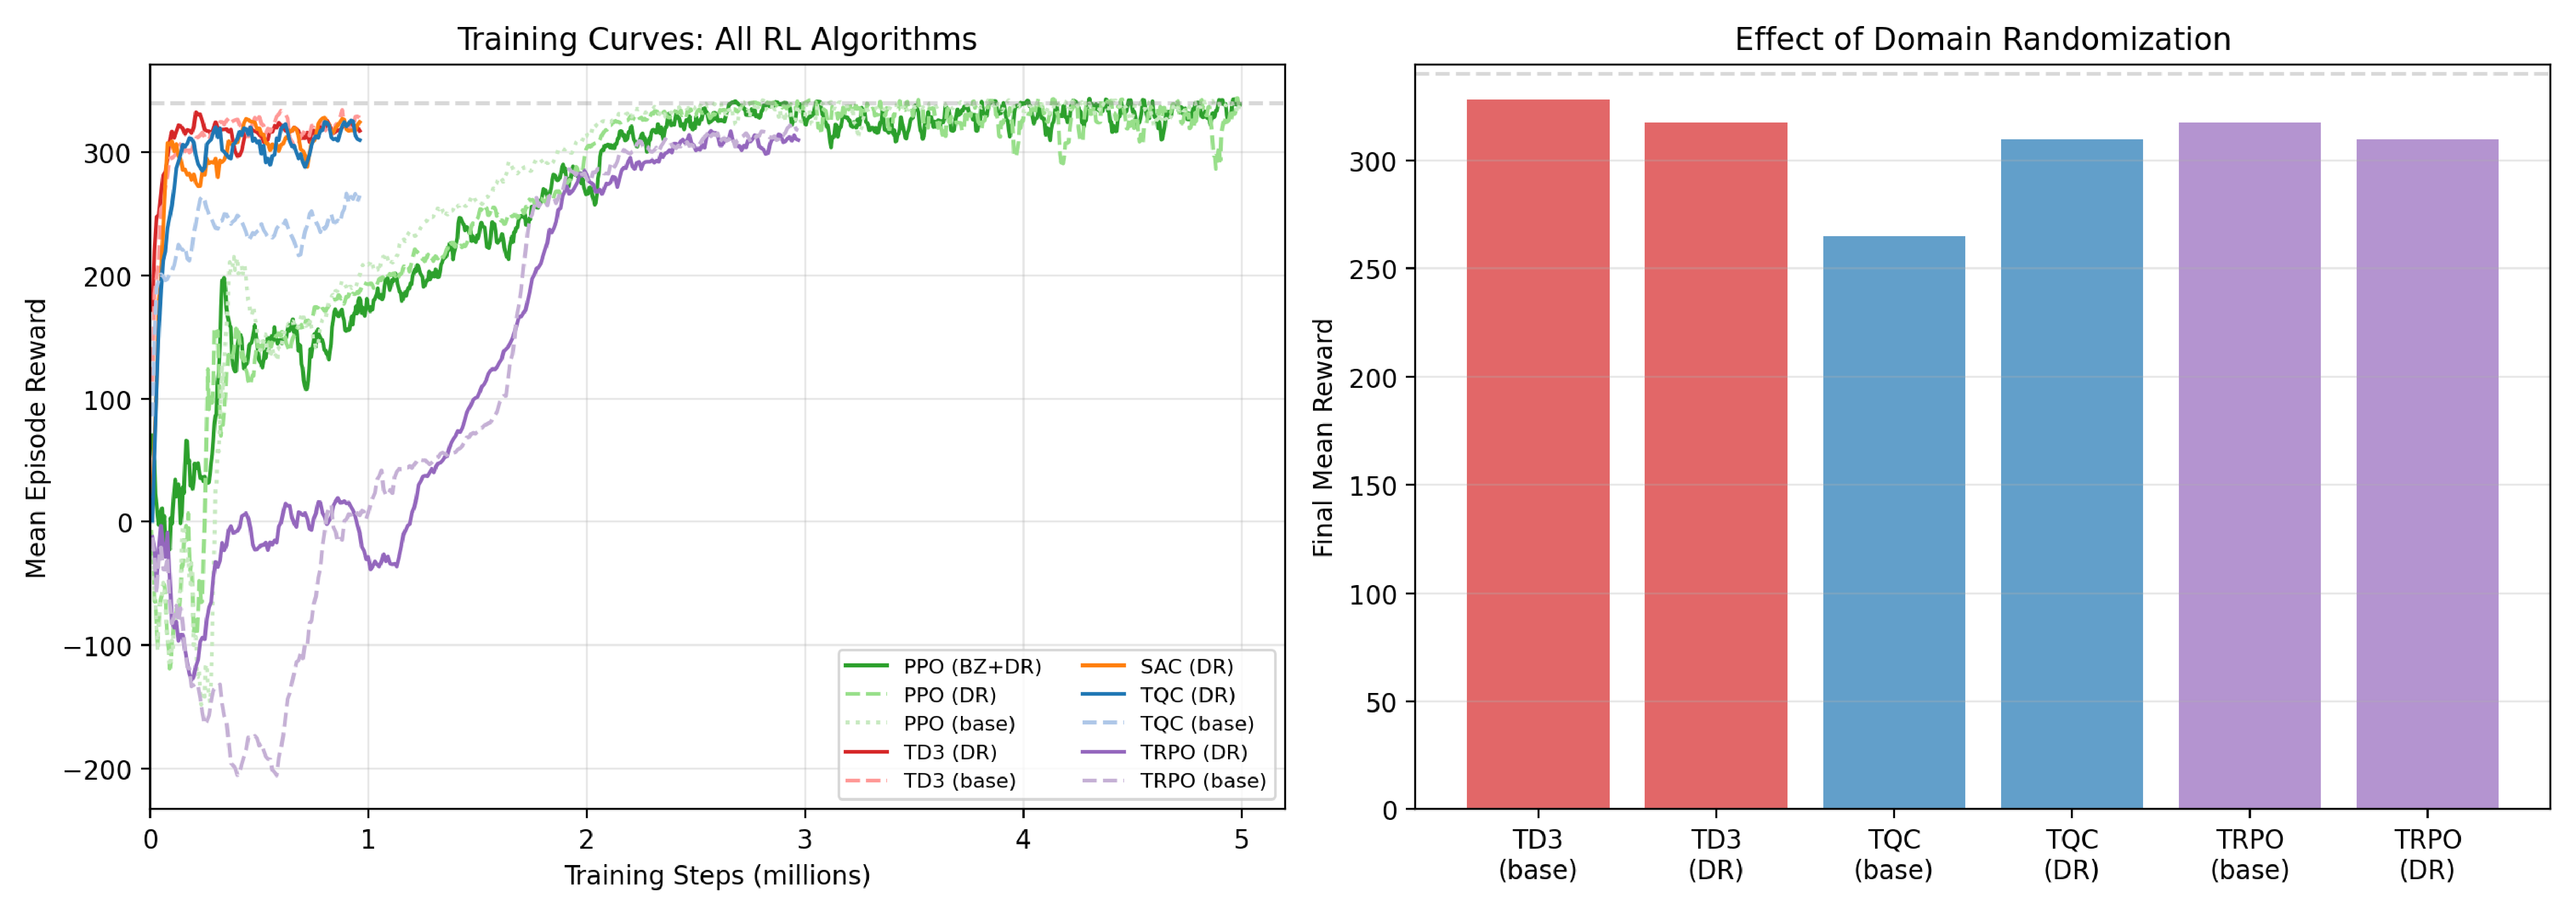
\includegraphics[width=\columnwidth]{figures/training_curves_all.eps}
  \caption{Left: Training curves (mean eval reward vs.~steps) for all
    RL algorithms.  Right: Effect of domain randomization on final
    reward.  DR slightly reduces sim performance but improves
    real-world success (see Appendix~\ref{appendix:multi_algo_hw}).}
  \label{fig:training_curves}
\end{figure}

\subsection{PPO Ablation Study}
\label{appendix:ppo_ablation}

We conducted a systematic ablation to identify which training
configuration factors most influence sim-to-real transfer quality.
We trained several PPO variants (3M steps each, S-curve motor,
seed~$=1$) and evaluated them on the same 50-trial stratified
initial-condition sequence used for the benchmark
(Section~\ref{sec:ic_design}). The ablation factors are the reward
function (balanced vs.~Gaussian), domain randomization (DR), and the
blind-zone sensor model (BZ); their combinations are listed in
Table~\ref{tab:ppo_ablation}.

All variants used the S-curve motor model and ball sensor staleness.

\subsubsection{Results}

Table~\ref{tab:ppo_ablation} reports the best checkpoint per variant
(selected by highest success rate, then fastest settling) evaluated
with 50 stratified trials, settling band $= 0.01$\,rad,
settling duration $= 1.0$\,s.

\begin{table*}[!t]
\centering
\renewcommand{\arraystretch}{1.15}
\caption{PPO ablation study: simulation (S-curve motor model). Every row
  except Gaussian is a 50-trial stratified evaluation from
  \texttt{rl\_ablation/blind\_zone\_ablation.json}; the Gaussian row is a
  20-trial checkpoint screen (seed 42) from
  \texttt{rl\_ablation/ppo\_checkpoint\_sweep.json}. ``Settle'' is the mean
  over successful trials; ``RMS Effort'' is the RMS commanded action
  averaged over trials (the Gaussian value is derived from the stored
  squared effort).}
\label{tab:ppo_ablation}
\begin{tabular}{lcccc}
\toprule
\textbf{Variant} & \textbf{Ckpt} & \textbf{SR} & \textbf{Settle (s)}
  & \textbf{RMS Effort} \\
\midrule
Balanced          & best  & 100\% & 1.72 & 0.078 \\
Gaussian          & final &  95\% & 2.22 & 0.731 \\
Balanced + BZ     & best  &  96\% & 2.37 & 0.145 \\
Balanced + BZ + DR& best  & 100\% & 1.67 & 0.096 \\
Balanced + DR     & final & 100\% & 1.49 & 0.076 \\
\bottomrule
\end{tabular}
\end{table*}

\subsubsection{Analysis}

\paragraph{Reward function.}
The composite \emph{balanced} reward achieves 100\% simulation
success with far lower control effort than the pure-Gaussian
reward (RMS effort 0.078 vs.\ 0.731). The Gaussian reward lacks
explicit effort and jerk penalties; its hardware validation
(Table~\ref{tab:ppo_hardware}, 30\% SR / 15.62\,s over 10 trials)
confirms that the oscillatory behavior translates directly to
real-world failure.

\paragraph{Blind-zone and domain randomization.}
Adding the blind-zone model alone (Balanced+BZ) drops simulation
SR slightly (96\%), consistent with the policy overfitting to a fixed
blind-zone threshold. Adding DR on top (Balanced+BZ+DR) recovers 100\%
simulation SR (1.67\,s); DR randomizes the blind-zone threshold together
with the physical and observation-noise parameters, so the recovery is not
attributable to threshold randomization alone. This is the configuration behind PPO~(BZ+DR). Its S-curve
policy reaches 98\% hardware SR over 50 trials, while the matched
first-order-lag checkpoint reported in Table~II (main paper) reaches 96\%
(Appendix~\ref{appendix:rl_fairness}).
DR alone (Balanced+DR) also reaches 100\% simulation SR with the
lowest control effort (0.076).

\paragraph{Training duration.}
Figure~\ref{fig:ppo_checkpoints} shows that 1--1.5M steps is the
best trade-off: at 500K steps all variants achieve $\leq 85$\% SR;
beyond $\sim$2M steps settling time increases as the policy becomes
more conservative without improving reliability.

\begin{figure}[!t]
  \centering
  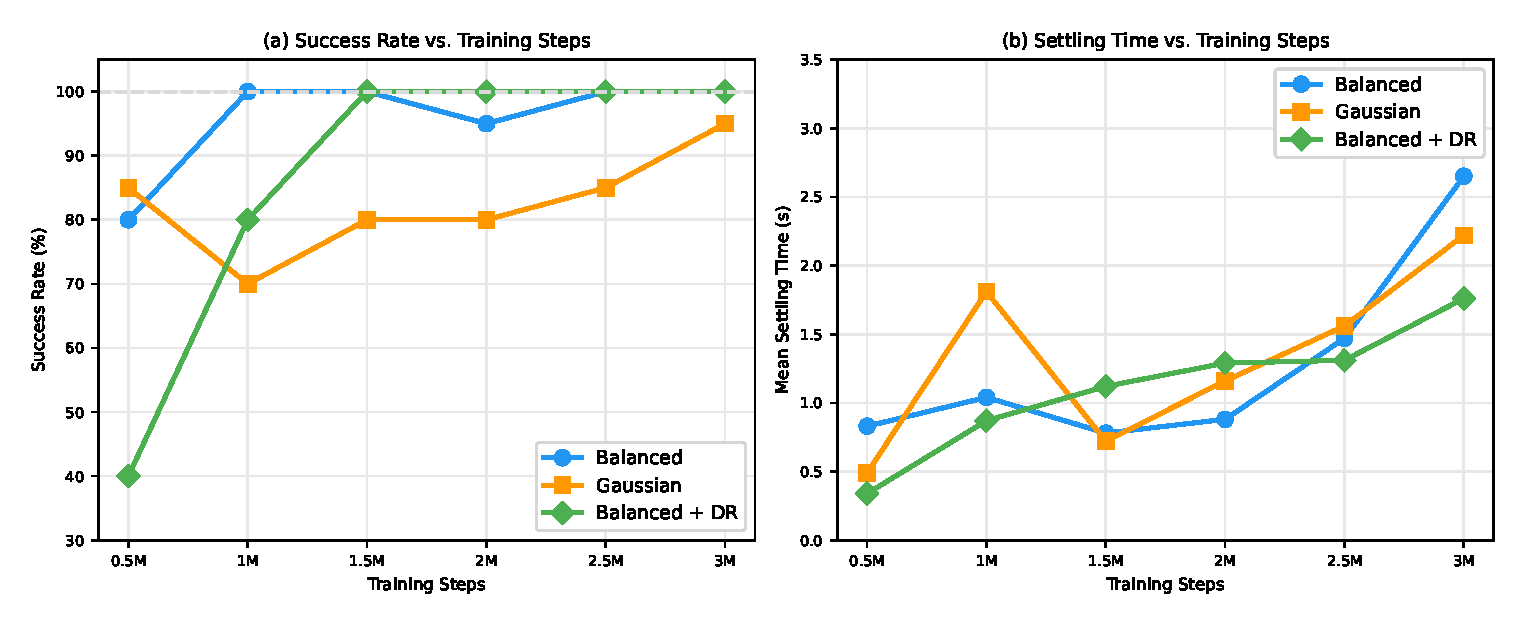
\includegraphics[width=0.99\columnwidth]{figures/ppo_ablation_checkpoints.eps}
  \caption{Success rate and mean settling time vs.~training
    checkpoint for the PPO variants.
    Balanced and Balanced+DR reach 100\% SR by 1--1.5M steps;
    Gaussian plateaus below 100\%.}
  \label{fig:ppo_checkpoints}
\end{figure}

\subsection{Hardware Validation of PPO Variants}
\label{appendix:ppo_hardware}

To validate the simulation ablation findings, we tested the top three PPO
variants on real hardware (10 trials each, stratified
initial conditions, identical protocol to Section~\ref{sec:ic_design}).

\begin{table*}[!t]
\centering
\renewcommand{\arraystretch}{1.15}
\caption{PPO hardware validation (10 trials per variant).}
\label{tab:ppo_hardware}
\begin{tabular}{lccc}
\toprule
\textbf{Variant} & \textbf{SR} & \textbf{Settle (s)}
  & \textbf{Max (s)} \\
\midrule
Balanced (no DR) & 100\% & 5.26 & 15.81 \\
Balanced + DR    & 100\% & 6.94 & 21.66 \\
Gaussian         &  30\% & 15.62 & 28.11 \\
\bottomrule
\end{tabular}
\end{table*}

\subsubsection{Hardware Insights}

\paragraph{Reward function on hardware.}
The Gaussian-reward policy fails 70\% of hardware trials, confirming
that the aggressive oscillatory behavior observed in simulation
translates directly to real-world failure.
The composite \emph{balanced} reward's effort and jerk penalties
produce smooth, hardware-compatible control signals.

\paragraph{Sim-to-real settling gap.}
Hardware settling times are 3--5$\times$ slower than simulation
(sim: 1.5--1.7\,s $\to$ hw: 5.3--6.9\,s).
The simulation-to-hardware characterization in
Appendix~\ref{appendix:simulation_validation} identifies plausible
contributors to this gap: sensor characteristics (the $\sim$82\,ms ToF cycle
and the $|\theta|>0.071$\,rad saturation) and the higher-order motor
response (the S-curve profile approximated as first-order lag); ball-arc
friction and the uncontrolled initial ball velocity likely add further
variance. This is inferred from the open-loop prediction analysis rather
than a controlled controller-level ablation.

\paragraph{Domain randomization: sim-to-real trade-off.}
Both balanced variants achieve 100\% hardware success rate.
In simulation, DR is \emph{faster} (1.49 vs.\ 1.72\,s) due to
its regularization effect.
On hardware, this inverts: the no-DR model settles 24\% faster
(5.26 vs.\ 6.94\,s), consistent with the real system being close to the
nominal parameters it was trained on.
The DR model's policy is smoother but more cautious on the
real system.
For long-term deployment where hardware properties may drift
(mechanical wear, temperature drift), DR is plausibly the more robust
choice, though we did not run a drift experiment to confirm this.

\subsection{Multi-Algorithm Comparison}
\label{appendix:multi_algo}

We trained five RL algorithms with the \emph{balanced} reward, each
in two variants (base: nominal dynamics; DR: domain randomization).
On-policy algorithms (PPO, TRPO~\cite{schulman2015trpo}) used 16 parallel
environments; off-policy algorithms (SAC~\cite{haarnoja2018sac},
TD3~\cite{fujimoto2018td3}, TQC~\cite{kuznetsov2020controlling})
used 1 environment.
PPO and TRPO use two-layer MLPs with $[64,64]$ hidden units; SAC and TQC use
the Stable-Baselines3 default of $[256,256]$, and TD3 uses its default of
$[400,300]$. Each algorithm therefore keeps its library
default rather than a hand-tuned network. All five algorithms were trained
with the same single seed (seed~1) under the deterministic Hydra
configuration (\texttt{training/configs/train.yaml}), so cross-algorithm
differences are not confounded by seed choice; per-algorithm
training-stochasticity variance is not characterized.
Table~\ref{tab:rl_training_cost} summarizes the training cost;
Table~\ref{tab:rl_comparison} reports simulation evaluation.

\paragraph{Model selection.}
For each training run, all saved checkpoints are evaluated through
simulation (50 trials, stratified ICs). Three models are selected
for hardware deployment: (1)~the checkpoint with the highest
simulation success rate, (2)~the final checkpoint at the end of
training, and (3)~an intermediate checkpoint that achieves good
performance without being the absolute best or final (to capture
potential overfitting). The model that performs best on hardware
is reported in the main results. SB3's \texttt{EvalCallback}
(10 deterministic episodes every 50K steps) is used only for
training progress monitoring, not for final model selection.

\begin{table*}[!t]
\centering
\renewcommand{\arraystretch}{1.15}
\caption{Training cost per algorithm (Intel i5, CPU only).}
\label{tab:rl_training_cost}
\begin{tabular}{lccccc}
\toprule
\textbf{Algorithm} & \textbf{Type} & \textbf{$n_\text{envs}$}
  & \textbf{Steps} & \textbf{Wall-clock} & \textbf{$\geq$300 step} \\
\midrule
PPO   & on-policy  & 16 & 3.0M & $\sim$40\,min   & 1.35--2.0M \\
TRPO  & on-policy  & 16 & 3.0M & $\sim$58\,min   & 1.0--1.35M \\
SAC   & off-policy &  1 & 1.0M & $\sim$5.7\,h    & 150--250K \\
TD3   & off-policy &  1 & 1.0M & $\sim$5.7\,h    & 50--250K \\
TQC   & off-policy &  1 & 1.0M & $\sim$8.5\,h  & 100--200K \\
\bottomrule
\end{tabular}
\end{table*}

\noindent
The ``$\geq$300 step'' column indicates the first training step at which
the evaluation reward exceeded 300 (a functional policy threshold;
theoretical maximum is 360 for 600 steps).
On-policy methods are faster in wall-clock time due to 16-environment
parallelism despite requiring more total environment steps.
Among the off-policy methods (single environment), TD3 reaches the
functional-policy threshold in the fewest steps (from about 50K), while
TQC has the longest wall-clock time (about 8.5\,h).

\begin{table*}[!t]
\centering
\renewcommand{\arraystretch}{1.15}
\caption{Multi-algorithm comparison: simulation (50 trials, first-order motor model)
  and hardware (50 stratified trials) success rate and settling time.
  Sim settling is computed over successful trials; hardware SR ranges from 60--96\%.}
\label{tab:rl_comparison}
\begin{tabular}{lccccc}
\toprule
\textbf{Model} & \textbf{SR} & \textbf{Sim Mean (s)} & \textbf{Med.\,(s)}
  & \textbf{HW SR} & \textbf{HW Mean (s)} \\
\midrule
PPO (base)  & 100\% & 1.72 & 1.25 & 60\%  & 3.53 \\
PPO (BZ+DR) &  96\% & 0.82 & 0.40 & 96\%  & 3.81 \\
SAC (DR)    & 100\% & 0.98 & 0.60 & 82\%  & 10.10 \\
TD3 (DR)    & 100\% & 1.78 & 0.55 & 92\%  & 11.45 \\
TQC (DR)    & 100\% & 1.89 & 0.60 & 86\%  & 9.77 \\
TRPO (DR)   & 100\% & 3.88 & 2.18 & 90\%  & 8.09 \\
\bottomrule
\end{tabular}
\end{table*}

\subsubsection{Algorithm Analysis}

The simulation settling times in Table~\ref{tab:rl_comparison} are those of
the \emph{deployed} checkpoints (the same policies as in
Table~\ref{tab:full_results}), reproduced on the shipped models. The
blind-zone and domain-randomization ablations later in this appendix instead
report the S-curve development family (Appendix~\ref{appendix:rl_fairness}),
whose simulation settling differs accordingly; the two should not be compared
directly.

\paragraph{PPO and SAC settling time.}
At their deployed checkpoints, PPO~(BZ+DR) has the fastest simulation
settling (0.82\,s) among these configurations, at 96\% SR; SAC~(DR)
reaches 100\% SR and settles in 0.98\,s mean (0.60\,s
median). PPO also has lower control effort. The 16-environment
parallelism makes PPO the most wall-clock efficient (40\,min vs.\
90+\,min for SAC).

\paragraph{SAC with DR and longer training.}
At its deployed checkpoint SAC~(DR) settles in 0.98\,s (simulation) at
100\% SR. SAC reaches a functional policy (reward $\geq 300$) in about
150K steps (Table~\ref{tab:rl_training_cost}), fewer than PPO, and both
domain randomization and longer training improve settling relative to
shorter runs.

\paragraph{TD3 across training budgets.}
At its deployed checkpoint TD3~(DR) settles in 1.78\,s (simulation) at
100\% SR, and longer training improves settling over shorter budgets.
TD3~(DR) converges fastest of all algorithms
(reward $\geq 300$ at 50K steps, Table~\ref{tab:rl_training_cost}).

\paragraph{TQC across training budgets.}
At its deployed checkpoint TQC~(DR) reaches 100\% SR with 1.89\,s mean
settling (simulation). Its truncated quantile critics (25 atoms per
critic) require more training budget than SAC or TD3 to reach strong
performance, but converge to a reliable policy given enough training.

\paragraph{TRPO and DR.}
At 3M steps, the deployed TRPO~(DR) checkpoint reaches 100\% simulation
SR with 3.88\,s mean settling, the slowest of the DR agents.
TRPO~(base) drops to 90\% SR with longer training,
suggesting overfitting to nominal dynamics.
The conservative trust-region updates produce smooth control
(ISE$_u \approx 0.03$) but cannot match PPO/SAC speed.

\subsubsection{Failure Mode Analysis}

Across the seven simulation-trained RL controllers evaluated with 50
hardware trials each (350 trials total), the dominant predictor of failure is
the training configuration, not the initial-condition stratum
(Tables~\ref{tab:full_results} and~\ref{tab:failed_variants}), and the stratum pattern that does appear runs
opposite to the expectation that the most constrained starts are the
hardest:

\paragraph{Blind-zone modeling and DR.}
The base PPO policy (no DR, no BZ) fails on 20/50 trials (60\% SR);
adding DR reduces this to 5/50 (PPO~(DR), 90\%), and adding both DR
and the blind-zone model reduces it to a single failure
(PPO~(BZ+DR), 98\% in the S-curve training family;
Appendix~\ref{appendix:rl_fairness}). SAC~(DR)
(82\%, 9 failures) and TQC~(DR) (86\%, 7 failures), which are not
trained with the blind-zone model, fail more often than PPO~(BZ+DR),
consistent with the blind-zone being a contributing cause of RL
hardware failures.

\paragraph{Failure distribution across strata.}
Contrary to the expectation that the most constrained starts are the hardest,
the failures spread across strata, and the at-wall-opposite start is among the
easiest rather than the hardest. The center and mid-rail starts draw as many
failures as the constrained ones or more: the single PPO~(BZ+DR) failure of the
S-curve development checkpoint is on a center start (cart at $-0.09$\,m), not at
a wall (the deployed first-order-lag checkpoint of Table~\ref{tab:full_results}
instead misses two at-wall-same trials), and TD3 and TRPO also miss on center. This echoes the pattern that the center and
mid-rail starts, despite offering the most maneuvering room, are where these
RL controllers fail most: with the cart already positioned and no wall to use
as a momentum backstop, the controller must wait out the ball's own dynamics.

\subsubsection{Full Hardware Evaluation (50 Trials)}
\label{appendix:multi_algo_hw}

Every model-free RL algorithm (the DR variant of each off-policy method,
together with PPO~(BZ+DR)) was evaluated on hardware over the full 50
stratified trials (same protocol as Section~\ref{sec:ic_design}).

\begin{table*}[!t]
\centering
\renewcommand{\arraystretch}{1.15}
\caption{Full hardware evaluation: RL models (50 trials each,
         stratified ICs).}
\label{tab:rl_hw_50trial}
\begin{tabular}{lccccc}
\toprule
\textbf{Model} & \textbf{HW SR} & \textbf{Settle (s)}
  & \textbf{Med (s)} & \textbf{Max (s)} & \textbf{Sim SR} \\
\midrule
PPO (BZ+DR) & 96\% & 3.81 & 3.15 & 13.90 & 96\% \\
TD3 (DR)    & 92\% & 11.45 & 10.06 & 28.11 & 100\% \\
TRPO (DR)   & 90\% & 8.09 & 4.80 & --  & 100\% \\
PPO (DR)    & 90\% & 5.11 & 2.55 & 22.85 & 100\% \\
TQC (DR)    & 86\% & 9.77 & 6.61 & --  & 100\% \\
SAC (DR)    & 82\% & 10.10 & 8.40 & --  & 100\% \\
PPO (base)  & 60\% & 3.53 & 2.53 & 10.55 & 100\%  \\
\bottomrule
\end{tabular}
\end{table*}

\paragraph{50-trial results.}
Over the full 50-trial evaluation (Table~II, main paper),
PPO~(BZ+DR) achieves 96\% SR, with two failures on at-wall-same trials.
PPO~(DR) achieves 90\% SR. In the matched S-curve development ablation,
adding the blind-zone model lifts PPO~(BZ+DR) from 90\% to 98\%
(+8 percentage points); the deployed first-order-lag checkpoint of
Table~II reaches 96\%.
PPO~(base) at 60\% indicates that domain randomization is important
for sim-to-real transfer at this training budget (single training seed).

\subsection{Extended Training: 5M-Step Ablation}

While the main 3M-step ablation shows that blind-zone modeling is
the efficient path to high hardware SR, we also evaluated PPO
variants at extended timesteps on hardware (50 trials each,
Table~\ref{tab:ppo_5m_hw}):

\begin{table}[H]
\centering
\caption{PPO 5M-step hardware evaluation (50 trials, 20\,Hz).}
\label{tab:ppo_5m_hw}
\begin{tabular}{lccc}
\toprule
\textbf{Variant} & \textbf{Steps} & \textbf{HW SR} & \textbf{Median (s)} \\
\midrule
PPO base (no DR, no BZ)  & 5.0M  & 100\% & 3.05 \\
PPO BZ+DR                & 2.75M & 96\%  & 3.15 \\
PPO BZ+DR                & 3.50M & 94\%  & 3.30 \\
PPO DR                    & 2.25M & 84\%  & 4.55 \\
\bottomrule
\end{tabular}
\end{table}

Base PPO at 5M steps (first-order motor model) achieves 100\% SR with no
domain randomization and no blind-zone modeling, above the 3M base
variant (60\%). This suggests extended training can partly compensate for
missing sensor awareness, though the two baselines differ in motor regime
(first-order vs.\ S-curve development) and each is a single checkpoint, so
the comparison is not fully controlled.
However, PPO~(BZ+DR) at 3M steps remains the more time-efficient
approach (98\% SR in $\sim$40\,min vs.\ 100\% SR in $\sim$67\,min).
BZ+DR performance is slightly lower at 3.5M steps (94\%). PPO~(DR) at
2.25M steps underperforms the 3M DR variant (84\% vs.\ 90\%). These are
single-checkpoint point estimates, so we report them as observations rather
than controlled trends.

\noindent In these runs, sensor modeling (BZ) and extended training
each improved the observed sim-to-real transfer. BZ
offers training efficiency (98\% at 3M), while extended training
reaches higher reliability (100\% at 5M) at the cost of longer
training time.

\paragraph{Simulation vs hardware ranking.}
SAC~(DR) reaches 100\% simulation SR but only 82\% hardware SR over
50 trials, the most aggressive sim-to-real gap among the RL controllers
that still achieve 100\% simulation SR, suggesting its policy exploits
simulation dynamics that do not transfer.
TRPO's conservative trust-region updates leave it too cautious to
recover from some real perturbations within the 30\,s time limit;
it nonetheless reaches 90\% SR over 50 trials.

\paragraph{TD3 and longer training.}
The deployed TD3~(DR) checkpoint (1M steps) reaches 92\% SR over the
full 50-trial evaluation. TD3 transfers to hardware better than SAC
but still cannot match PPO's robustness.

\paragraph{Overall ranking.}
PPO's on-policy training with 16 parallel environments produces
policies that generalize to hardware most reliably.
The combination of PPO + DR + blind-zone modeling achieves
96\% SR over 50 hardware trials with 3.81\,s mean settling (the
first-order-lag checkpoint of Table~II, main paper).
No off-policy algorithm matches this: TD3~(DR) is closest
at 92\% SR but with about three times the settling time (11.45\,s).

\subsection{Sensor Blind Zone Ablation}
\label{appendix:blind_zone}

The VL53L0X sensor exhibits a minimum-range blind-zone
(Appendix~\ref{appendix:sensor_characterization}): when the ball
is within $\sim$40\,mm of a sensor ($|\theta| > 0.071$\,rad),
the reading saturates and the controller observes the ball
``stuck'' at the boundary.
We introduced an optional blind-zone model in the training
environment (Appendix~\ref{appendix:sensor_sim_model}) and trained two
additional PPO variants: one with blind-zone only (BZ), one with
both blind-zone and domain randomization (BZ+DR).

\begin{table*}[!t]
\centering
\renewcommand{\arraystretch}{1.15}
\caption{Blind zone ablation: simulation evaluation
         (50 trials, evaluated \emph{without} blind-zone to isolate
         control quality).}
\label{tab:blind_zone_sim}
\begin{tabular}{lccccc}
\toprule
\textbf{Training Config} & \textbf{BZ} & \textbf{DR}
  & \textbf{SR} & \textbf{Settle (s)} \\
\midrule
Balanced          & No    & No    & 100\% & 1.72 \\
Balanced + DR     & No    & Yes & 100\% & 1.49 \\
Balanced + BZ     & Yes & No    &  96\% & 2.37 \\
Balanced + BZ+DR  & Yes & Yes & 100\% & 1.67 \\
\bottomrule
\end{tabular}
\end{table*}

\begin{table*}[!t]
\centering
\renewcommand{\arraystretch}{1.15}
\caption{Blind zone ablation: hardware validation (10 trials each).}
\label{tab:blind_zone_hw}
\begin{tabular}{lccccc}
\toprule
\textbf{Training Config} & \textbf{BZ} & \textbf{DR}
  & \textbf{SR} & \textbf{Settle (s)} & \textbf{Max (s)} \\
\midrule
Balanced          & No    & No    & 100\% & 5.26 & 15.81 \\
Balanced + DR     & No    & Yes & 100\% & 6.94 & 21.66 \\
Balanced + BZ     & Yes & No    &  60\% & 2.72 &  9.46 \\
Balanced + BZ+DR  & Yes & Yes & 100\% & 4.98 & 13.66 \\
\bottomrule
\end{tabular}
\end{table*}

\paragraph{Blind-zone model and DR.}
Without DR, the blind-zone model makes training harder (96\% sim SR,
60\% hardware SR): the policy overfits to a fixed blind-zone
threshold and cannot generalize to the real sensor's variable
minimum range.
With DR (which randomizes the threshold over
$[0.060, 0.080]$\,rad), the policy achieves 100\% hardware SR
and settles 28\% faster than the previous best (4.98 vs.\ 6.94\,s).

\paragraph{Sim-to-real gap.}
The settling-time ratio (hardware/sim) improves from
$4.7\times$ (no BZ: $6.94/1.49$) to $3.0\times$ (BZ+DR:
$4.98/1.67$), consistent with the blind-zone model
capturing part of the sim-to-real gap (single training seed).

\subsection{Complete Ablation Summary}
\label{appendix:ablation_summary}

Table~\ref{tab:full_ablation} consolidates all PPO ablation
variants with both simulation and hardware results, and
Fig.~\ref{fig:ppo_ablation_summary} shows the same comparison visually: the
Balanced+BZ+DR variant achieves the best combined performance, 100\% hardware
SR at the lowest sim-to-real settling gap (3.0$\times$).

\begin{table*}[!t]
\centering
\renewcommand{\arraystretch}{1.15}
\caption{Complete PPO ablation: simulation (50 trials, except the
         Gaussian-wall row, a 20-trial checkpoint screen) and
         hardware (10 trials). All variants trained for 3M steps
         with balanced reward unless noted.}
\label{tab:full_ablation}
\begin{tabular}{lcc|cc}
\toprule
 & \multicolumn{2}{c|}{\textbf{Simulation}} & \multicolumn{2}{c}{\textbf{Hardware}} \\
\textbf{Variant} & \textbf{SR} & \textbf{Settle} & \textbf{SR} & \textbf{Settle} \\
\midrule
Balanced (base)         & 100\% & 1.72\,s & 100\% & 5.26\,s \\
Balanced + DR           & 100\% & 1.49\,s & 100\% & 6.94\,s \\
Gaussian                &  95\% & 2.22\,s &  30\% & 15.62\,s \\
Balanced + BZ           &  96\% & 2.37\,s &  60\% &  2.72\,s \\
\textbf{Balanced + BZ+DR} & \textbf{100\%} & \textbf{1.67\,s} & \textbf{100\%} & \textbf{4.98\,s} \\
\bottomrule
\end{tabular}
\end{table*}

\begin{figure}[!t]
  \centering
  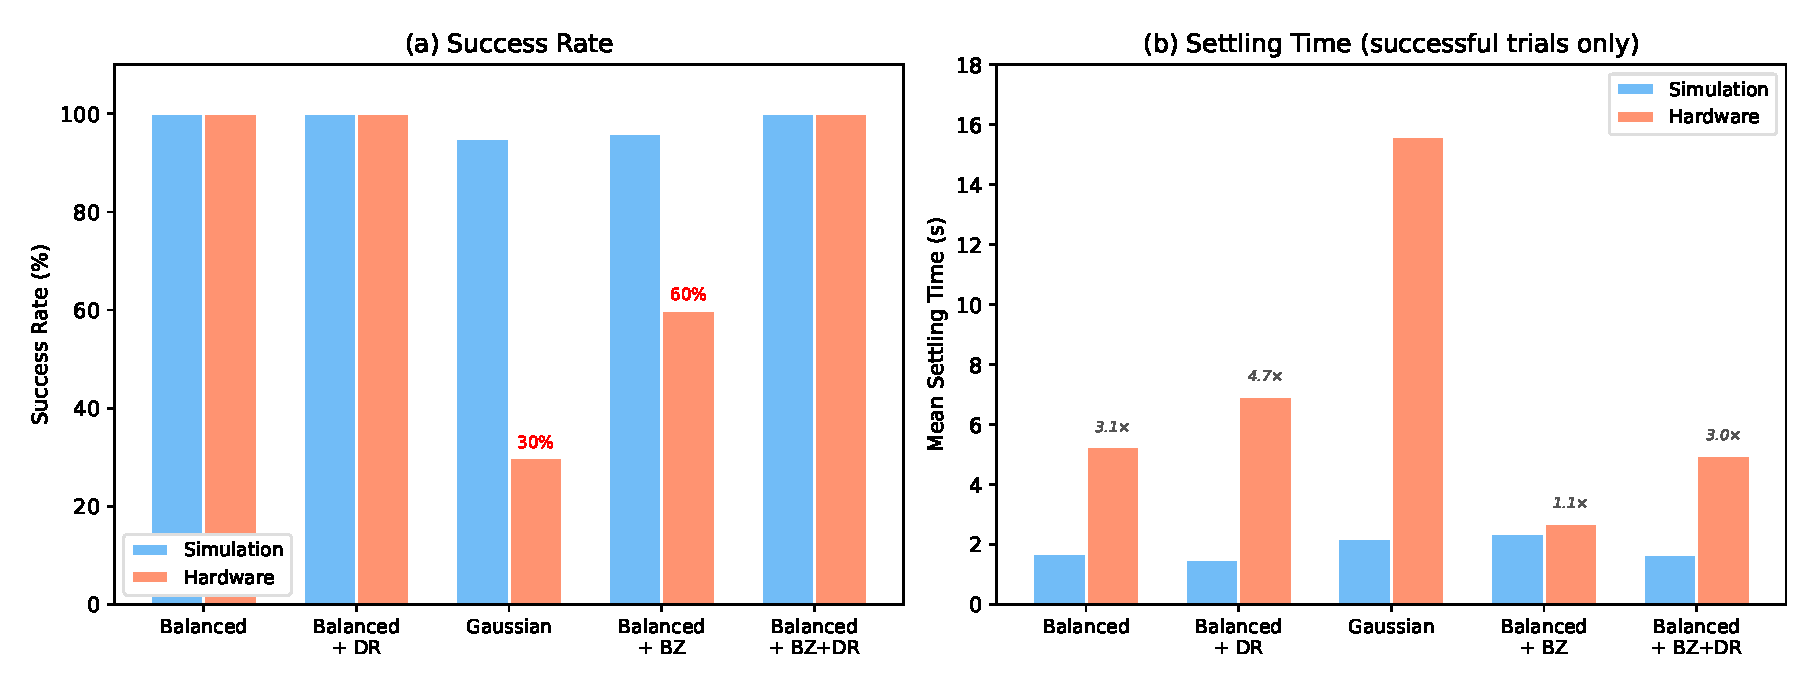
\includegraphics[width=0.99\columnwidth]{figures/ppo_ablation_summary.eps}
  \caption{Complete PPO ablation summary: success rate (a) and mean
    settling time (b) across simulation and hardware.
    Annotations in (b) show the sim-to-real settling ratio.
    The Balanced+BZ+DR variant achieves the best combined
    performance: 100\% hardware SR with the lowest sim-to-real gap
    (3.0$\times$).}
  \label{fig:ppo_ablation_summary}
\end{figure}

\subsection{Selected Model}
\label{appendix:selected_model}

Based on the complete ablation (Table~\ref{tab:full_ablation}), the
deployed PPO controller (Table~II in the main paper, reported as
PPO~(BZ+DR)) uses:
\begin{itemize}
  \item \textbf{Motor model:} The PPO~(BZ+DR) reported in Table~II of the
        main paper is the matched first-order-lag checkpoint, the same
        model used for the other four RL agents
        (Appendix~\ref{appendix:rl_fairness}). The S-curve profile
        (jerk-limited, mirroring the drive's internal profiler) was the
        development regime used for the ablations elsewhere in this
        supplement (Appendix~\ref{appendix:motor_fwhm_ablation},
        Table~\ref{tab:fwhm20_hw_10t}).
  \item Reward: \emph{balanced} (Eq.~\ref{eq:reward})
  \item Domain randomization: enabled
  \item Sensor blind-zone model: enabled
  \item Observation: standard 4-dimensional state
    $[x, \dot{x}, \theta, \dot{\theta}]$
  \item Training: extended sweep, best checkpoint at 2.75M steps
    (matched first-order-lag, Table~\ref{tab:ppo_5m_hw})
\end{itemize}

In simulation (50 trials): 100\% SR, mean settling 1.67\,s.
On hardware (50 trials), the matched first-order-lag checkpoint reported
in Table~II reaches 96\% SR, mean settling 3.81\,s (two failures); the
S-curve development policy reaches 98\%, 5.11\,s.

This configuration gives the highest hardware reliability among the
simulation-trained model-free RL controllers. In the development ablation, blind-zone modeling
lowers the sim-to-real settling gap from 4.7$\times$ (without it, $6.94/1.49$) to
3.0$\times$ ($4.98/1.67$).

\subsection{Motor Model and Dip-Width (FWHM) Ablation}
\label{appendix:motor_fwhm_ablation}

The original PPO models were trained with an S-curve motor profile
and a dip width of FWHM$= 42$\,mm in the simulation environment.
After independent measurement of the physical dip (FWHM$\approx 20$\,mm,
measured via sensor calibration), we conducted a systematic ablation
of these two training-environment parameters.

\subsubsection{Training configurations}

Two PPO training regimes were compared at FWHM$=20$\,mm:
\begin{enumerate}
  \item \textbf{FWHM=20, S-curve, 3M}: the original motor model,
    four sub-variants (base, DR, BZ+DR, Gaussian-wall).
  \item \textbf{FWHM=20, first-order, 5M}: the simplified
    first-order-lag motor model (no jerk/acceleration limits), trained
    for 5M steps, four sub-variants (base, DR, BZ+DR, Gaussian-wall).
\end{enumerate}

\subsubsection{Hardware screening (10 trials)}

Table~\ref{tab:fwhm20_hw_10t} reports the 10-trial hardware screening
for both regimes (data file: \texttt{rl\_finetuning/fwhm20\_ablation\_summary.json}).
This is a screening comparison, not the definitive 50-trial benchmark
of Table~II (main paper).

\begin{table*}[!t]
\centering
\renewcommand{\arraystretch}{1.15}
\caption{FWHM=20\,mm ablation, 10-trial hardware screening.
  SR and mean settling (successful trials) for S-curve-trained vs.
  first-order-trained PPO variants.}
\label{tab:fwhm20_hw_10t}
\begin{tabular}{lcccc cc}
\toprule
 & & \multicolumn{2}{c}{\textbf{S-curve trained}} & \multicolumn{2}{c}{\textbf{first-order trained}} \\
\cmidrule(lr){3-4}\cmidrule(lr){5-6}
\textbf{Variant} & & SR & Settle (s) & SR & Settle (s) \\
\midrule
PPO base          & & 100\% & 8.14 & 100\% & 11.06 \\
PPO +DR           & &  80\% & 6.33 &  90\% &  5.45 \\
PPO +BZ+DR        & &  90\% & 5.11 &  90\% &  6.58 \\
PPO Gaussian-wall & &  90\% & 6.14 &  80\% & 12.84 \\
\bottomrule
\end{tabular}
\end{table*}

\paragraph{FWHM=20\,mm vs.\ 42\,mm.}
On 10-trial screening the FWHM=20\,mm variants are competitive with
the deployed FWHM=42\,mm variants (whose S-curve 50-trial result is
PPO~(BZ+DR) 98\%/5.11\,s; Table~II (main paper) reports the matched
first-order-lag checkpoint at 96\%/3.81\,s). The dip-width
mismatch does not measurably degrade hardware performance at the 10-trial screening level (single training seed);
this is consistent with domain randomization varying the dip parameters
during training regardless of the nominal value.

\paragraph{First-order vs.\ S-curve training.}
Figure~\ref{fig:ppo_fo_5M_reward} shows the training-reward curves for
the three first-order 5M variants (eval reward, 20 deterministic episodes
every 5K steps; data files: \texttt{rl\_5m\_ablation/training\_runs/ppo\_fo\_5M\_*}).
All three converge to near-theoretical-maximum reward by ~2--3M steps and
remain stable through 5M, with the DR and BZ+DR variants reaching the
plateau slightly later than base. We report training-reward curves rather
than per-checkpoint hardware SR here because the per-checkpoint 50-trial
hardware evaluation of the first-order 5M checkpoints is not included in
this preprint; the deployed PPO~(BZ+DR) reported in Table~II (main paper) is the
matched first-order-lag checkpoint at 96\% SR; the S-curve
(3M, FWHM=42\,mm) policy reaches 98\% and is the development regime used
elsewhere in this supplement.

\begin{figure}[!t]
  \centering
  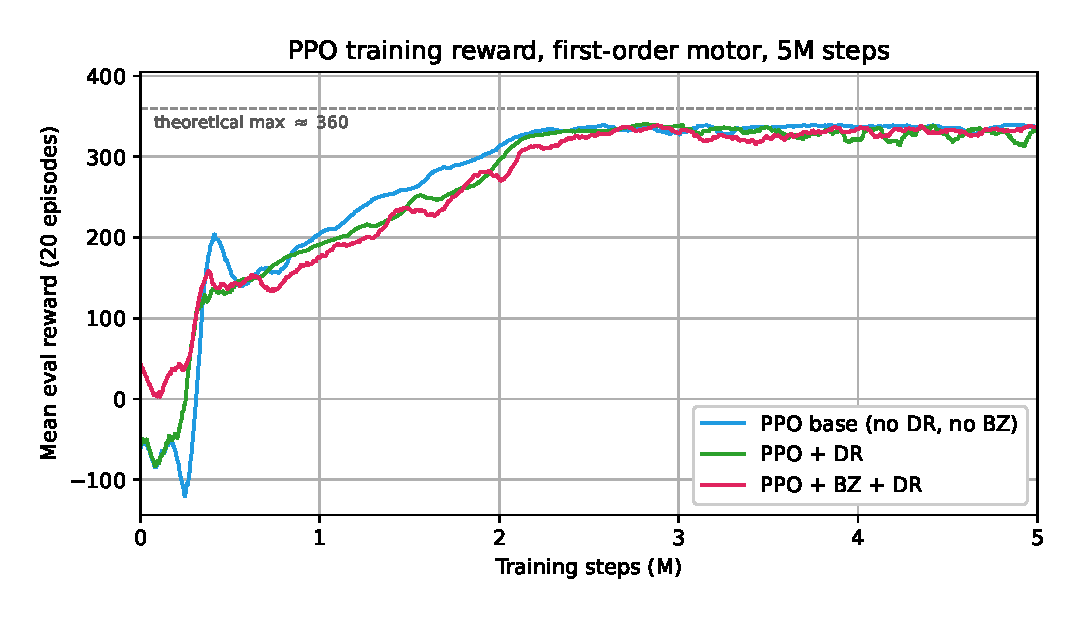
\includegraphics[width=\columnwidth]{figures/ppo_fo_5M_reward_curves.eps}
  \caption{First-order 5M PPO training-reward curves (mean eval reward
    vs.~training step, 20 episodes per checkpoint). Base, DR, and BZ+DR
    all plateau near the theoretical maximum (~360) by ~2--3M steps.
    }
  \label{fig:ppo_fo_5M_reward}
\end{figure}

\paragraph{FWHM mismatch.}
Training with FWHM$= 42$\,mm (2.1$\times$ the true value) does not
degrade hardware performance relative to the correct value.
This contrasts with NMPC, where the same conservative dip-width mismatch
materially helps hardware performance (Appendix~\ref{appendix:tuning_insights}).
For RL, the policy learns to handle the dip regardless of its
training-time width, provided domain randomization varies the dip
parameters during training.

\subsection{Fairness of the RL Comparison}
\label{appendix:rl_fairness}

The five simulation-trained RL agents in Table~II (main paper) are all
trained against the same first-order-lag motor model, but reaching that
consistency required a correction. An earlier PPO~(BZ+DR) policy used the
S-curve profile that mirrors the drive's internal profiler, whereas TD3,
SAC, TQC, and TRPO used the simplified first-order-lag approximation.
Because the S-curve is the closer match to the physical drive, that
asymmetry could in principle have flattered PPO.

To remove it, we re-trained PPO~(BZ+DR) under the same first-order-lag
model used for the other four agents and evaluated it over the identical
50-trial stratified protocol. The matched policy reaches 96\% hardware SR
(95\% CI $[87, 99]$, median settling 3.15\,s; best checkpoint of the
extended-training sweep, Table~\ref{tab:ppo_5m_hw}), and this is the
policy reported in Table~II. The earlier S-curve policy reaches 98\% and is
the one used elsewhere in this supplement, where the S-curve training
family is the consistent development regime: the fine-tuning study
(Appendix~\ref{appendix:finetuning}), the world-model comparison
(Appendix~\ref{appendix:world_model}), and the domain-randomization and
blind-zone ablations. Under either motor model PPO~(BZ+DR) remains the
most reliable and fastest-settling of the simulation-trained agents, so
the ranking and every qualitative finding are unchanged.

A second asymmetry concerns the blind-zone sensor model, added to PPO but
not to TD3, SAC, TQC, or TRPO. The off-policy agents take six to nine
hours each to train (Table~\ref{tab:rl_training_cost}), so the exhaustive
reward-and-sensor-model ablation that produced PPO~(BZ+DR) was practical
only for the on-policy PPO ($\sim$40\,min per run). We therefore read
PPO's lead as the strongest RL configuration we tested rather than
evidence that PPO is the best algorithm; the controlled claim, that
modeling the blind-zone helps, rests on the within-PPO ablation
(PPO~(DR) 90\% to PPO~(BZ+DR) 98\% in the matched S-curve ablation),
not on the cross-agent comparison.

\subsection{Simulation-to-Real Transfer}
\label{appendix:sim2real}

The trained policy is deployed on hardware without any online
fine-tuning or parameter adjustment (zero-shot transfer).
The primary sources of sim-to-real gap are:
\begin{enumerate}
  \item \textbf{Sensor blind-zone:} Near the arc boundaries
        ($|\theta| > 0.071$\,rad), the VL53L0X reports a saturated
        reading due to its minimum-range limitation
        ($\sim$30--50\,mm, Appendix~\ref{appendix:sensor_characterization}).
        The blind-zone model introduced in training reduces this gap
        from 4.7$\times$ to 3.0$\times$.
  \item \textbf{Sensor latency:} The ToF sensor cycle ($\sim$82\,ms)
        exceeds the control timestep (50\,ms), so the policy acts
        on ball-position measurements that may be one full
        sensor cycle old.
        This is modeled during training via stochastic ball-observation
        holding (mean staleness $= 2$ steps).
  \item \textbf{Residual unmodeled dynamics:} Higher-order motor
        nonlinearities (the Beckhoff 7-phase S-curve profile
        approximated as first-order lag) and asynchronous
        sensor-actuator timing account for the remaining
        $3.0\times$ settling-time ratio.
  \item \textbf{Sensor noise:} Inherent ToF noise
        ($\sigma \approx 1.6$--$1.7$\,mm) is captured
        via the observation noise model in domain randomization.
\end{enumerate}
The combination of S-curve motor model, ball sensor staleness,
blind-zone saturation model, and domain randomization gives
100\% success in the 10-trial hardware screening (the matched
first-order-lag checkpoint reaches 96\% over the full 50-trial
benchmark, the S-curve development policy 98\%), with a settling
gap of only 3.0$\times$.

\subsection{Offline Reinforcement Learning (IQL)}
\label{appendix:offline_rl}

In contrast to the simulation-trained online RL controllers above,
we evaluate Implicit Q-Learning (IQL)~\cite{kostrikov2022iql}
trained \emph{entirely on real hardware data}, with no simulated
transitions used for policy optimization.

\subsubsection{Dataset}

The IQL training dataset (\texttt{arcball\_post\_recalib\_flat.h5},
built by \texttt{data/build\_flat\_dataset.py}) contains
333,497 transitions from 1,415 hardware trials collected after sensor
recalibration (May 20+ 2026). It is a mixed dataset from all
controllers run on hardware during that period: MPPI, NMPC, RL variants
(PPO, TD3, SAC, TQC, TRPO), MPC, PD, LQR, SMC, and earlier offline-RL
checkpoints (104 trials from nine IQL checkpoints, none of them the
deployed \texttt{model\_280000}).
The dataset is 83\% successful and 17\% failed episodes.
This is \emph{not} expert-only data: it was collected during normal
hardware evaluation runs, not a dedicated data-collection phase.

The 222 source evaluation logs are released under
\texttt{evaluation/results/real/}, and the exact corpus is rebuilt by
\texttt{build\_flat\_dataset.py} over the recording window
2026-05-20 to 2026-05-28 15:03. That upper cutoff is 47 minutes before the
deployed checkpoint's benchmark run, so by construction none of IQL's 50
benchmark trials can appear in its training data; the released manifest
(\texttt{iql\_source\_manifest.csv}) lists all 106 contributing
controllers and contains no entry for the deployed \texttt{model\_280000}.
The training/evaluation split is therefore reproducible rather than assumed.

Rewards are recomputed offline using the balanced reward function
(Eq.~\ref{eq:reward}) with $\text{dip\_weight} = 1.0$. For training, the
transition stream is segmented into fixed 600-step episodes (30\,s at
20\,Hz) in recording order. Trials are much shorter than this (median
about 154 transitions), so nearly every window spans more than one trial
(552 of 555), and the fixed-length segmentation is a coarse approximation
of episode structure rather than an exact per-trial split.
Recovery behaviors are learnable from the successful episodes (83\%);
failed episodes provide coverage of near-boundary and initial transient
states but do not provide recovery signal.

\subsubsection{Algorithm Configuration}

IQL~\cite{kostrikov2022iql} is selected for its stability on
narrow datasets: it avoids querying out-of-distribution actions
by learning a separate value function $V(s)$ via expectile
regression and extracting the policy through advantage-weighted
behavioral cloning.
Key hyperparameters (Table~\ref{tab:iql_hyperparams}) follow the
original paper's recommendations.

\begin{table}[!t]
\centering
\renewcommand{\arraystretch}{1.15}
\caption{IQL hyperparameters (d3rlpy 2.8.1 implementation).}
\label{tab:iql_hyperparams}
\begin{tabular}{lcc}
\toprule
\textbf{Parameter} & \textbf{Value} & \textbf{Source} \\
\midrule
Policy architecture      & MLP [256, 256]   & d3rlpy default \\
Activation function      & ReLU             & d3rlpy default \\
Gradient steps           & 500\,000         & configured     \\
Batch size               & 256              & configured     \\
Discount $\gamma$        & 0.99             & default        \\
Actor learning rate      & $3{\times}10^{-4}$ & default      \\
Critic learning rate     & $3{\times}10^{-4}$ & default      \\
Number of critics        & 2                & default        \\
Soft-target $\tau$       & 0.005            & default        \\
Expectile                & 0.7              & default        \\
Weight temperature $\beta$ & 3.0            & default        \\
Max weight               & 100.0            & default        \\
Observation scaler       & Standard         & configured     \\
Action scaler            & MinMax           & configured     \\
\bottomrule
\end{tabular}
\end{table}

\subsubsection{Model Selection}

Checkpoints are saved every 10k gradient steps.
Because IQL is trained on real hardware logs, its behavior can differ
from our simulator, so simulation alone is not a reliable selector. We
first use 50-trial stratified simulation evaluation (same ICs as the
hardware protocol, first-order motor model) to shortlist checkpoints with
similar performance, then run about 10 hardware trials on each shortlisted
checkpoint to see which deploys best. The model at 280k steps gives the
best hardware result and is selected for deployment.

\subsubsection{Hardware Results}

\begin{table}[!t]
\centering
\renewcommand{\arraystretch}{1.15}
\caption{IQL hardware evaluation (model\_280000, 50 stratified trials).}
\label{tab:iql_hw_results}
\begin{tabular}{lccc}
\toprule
\textbf{Metric} & \textbf{SR} & \textbf{Mean (s)}
  & \textbf{Med (s) [IQR]} \\
\midrule
50 trials & 92\% & 10.62 & 9.80\,[4.49, 15.63] \\
10 trials (screening) & 100\% & 6.90 & 5.88 \\
\bottomrule
\end{tabular}
\end{table}

\paragraph{Difficulty breakdown.}
IQL achieves 100\% SR on medium (16/16), at-wall-opposite (5/5),
and at-wall-same (5/5) initial conditions.
Failures concentrate on easy/center (8/10, 80\%) and hard/near-wall (12/14,
86\%) strata, an unusual pattern among RL controllers.

\paragraph{Center-trial failures.}
IQL failed two center trials (cart at $\pm 0.10$\,m) while succeeding on
both at-wall strata. Center failures are not unique to IQL; several
online-RL controllers also miss center trials (for example, TD3 and SAC
each fail two). We did not retain per-step Q-values across the evaluation
set, so we report this as an observed pattern without a verified
mechanism.

\paragraph{Comparison with online RL.}
IQL reaches 92\% SR, matching TD3~(DR) (92\%) and well above PPO~(base)
(60\%), while training on real data alone; it is a few points below
PPO~(BZ+DR) (96\%). Success-rate gaps this small sit within the
benchmark's resolution (see the power analysis in the main paper), so we
read them as descriptive rather than a strict ordering. IQL's clearest
advantage is the lowest RMS control effort among the RL controllers
(0.395 vs.\ 0.492--0.680), producing smoother actuator commands.
Its median settling time (9.80\,s) is slower than TQC~(DR)
(6.61\,s) and much slower than PPO~(BZ+DR) (3.15\,s).

\paragraph{Significance.}
Achieving 92\% SR with a policy trained on only 333k real
transitions (280k gradient steps), without simulated training data,
domain randomization, or sensor modeling, demonstrates that
offline RL is a viable path when simulation fidelity is uncertain
or unavailable. The dataset of 1,415 post-recalibration trials
was collected during normal hardware evaluation runs; no dedicated
data-collection phase was required.

\section{World Model RL Training}\label{appendix:world_model}

This appendix reports on training PPO entirely inside a learned world model,
replacing the physics simulator with a data-driven dynamics model.

\subsection{World Model Architecture}

The world model is a 2-layer LSTM~\cite{hochreiter1997lstm}
(hidden dim $= 64$, sequence length $= 10$), implemented in
PyTorch~\cite{paszke2019pytorch} and trained on a 1\,M-transition
random-exploration dataset ($\sim$14 hours of operation; collection protocol
in Appendix~\ref{appendix:dataset_details}). Its input is the
concatenation of the current state
$\mathbf{s}_t = [x_c, \dot{x}_c, \theta_b, \dot{\theta}_b]$ and the action
$a_t$, and it predicts the state delta
$\Delta\mathbf{s}_{t+1} = \mathbf{s}_{t+1} - \mathbf{s}_t$, with normalization
statistics precomputed from the dataset (Fig.~\ref{fig:wm_arch}). We train it
for 50 epochs, reaching a final training-set prediction MAE of 0.611 in the
normalized state space.

\paragraph{Training hyperparameters.}
The model (hidden dim 64, 2 LSTM layers, dropout 0.2) is trained with the
Adam optimizer at learning rate $10^{-4}$, batch size 256, over
10-step sequences for 50 epochs. The objective is a per-dimension-weighted MSE
on the predicted state delta $\Delta\mathbf{s}$, with weights $[1, 5, 1, 5]$
on $[x_c, \dot{x}_c, \theta_b, \dot{\theta}_b]$ to emphasize the two velocity
channels. The 1\,M-transition collection is split $80/10/10$ into
train/validation/test, with normalization statistics computed on the training
split only, and all seeding uses seed~42. When MPPI plans with
this world model at deployment, we run it on CPU, which is faster than GPU for
a network this small on our target hardware, and the per-step planning cost
(about 40\,ms for 800 sampled rollouts over a horizon of 30) stays within the
50\,ms control period. PPO-WM instead deploys only its trained policy network,
so the world model runs online only under MPPI.

\begin{figure}[!t]
\centering
\resizebox{0.98\columnwidth}{!}{%
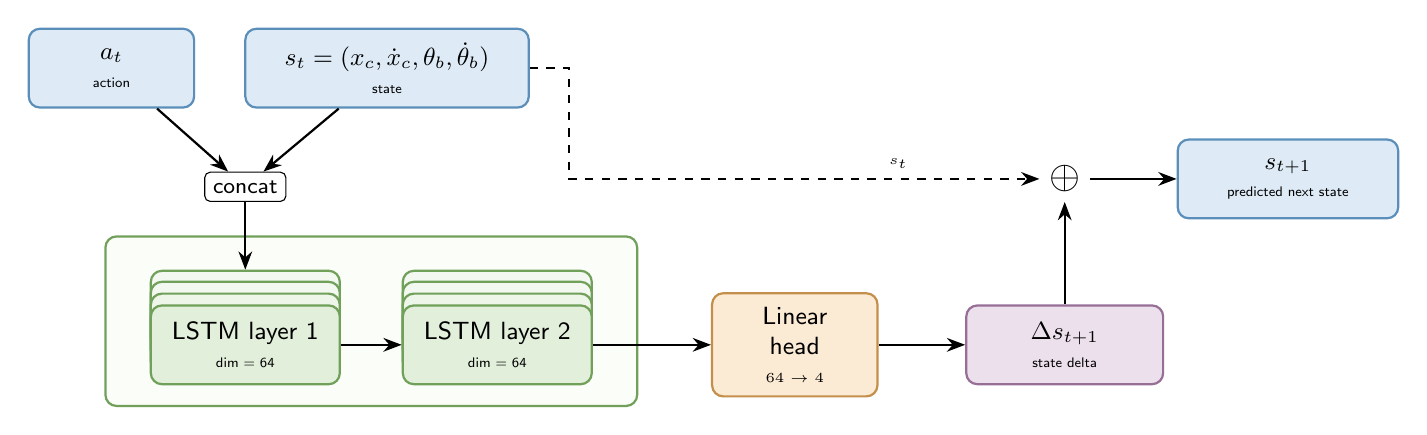
\begin{tikzpicture}[
    >=Stealth,
    every node/.style={font=\sffamily\small},
    box/.style={
        draw=black, thick, rounded corners, fill=white,
        minimum height=1.0cm, align=center, inner sep=5pt
    },
    flow/.style={draw=black, thick, -{Stealth}},
    skip/.style={draw=black, thick, dashed, -{Stealth}},
    node distance=0.9cm and 1.1cm
]
\definecolor{cInput}{RGB}{222,235,247}
\definecolor{cInputLine}{RGB}{91,143,185}
\definecolor{cLSTM}{RGB}{226,239,218}
\definecolor{cLSTMLine}{RGB}{112,160,90}
\definecolor{cHead}{RGB}{252,235,212}
\definecolor{cHeadLine}{RGB}{196,143,75}
\definecolor{cDelta}{RGB}{237,224,237}
\definecolor{cDeltaLine}{RGB}{150,110,150}
\definecolor{cOutput}{RGB}{222,235,247}
\definecolor{cOutputLine}{RGB}{91,143,185}

% Layer 1
\begin{scope}
  \node[box, fill=cLSTM!40, draw=cLSTMLine, minimum width=2.4cm,
        yshift=0.44cm] (lstm1b3) {};
  \node[box, fill=cLSTM!40, draw=cLSTMLine, minimum width=2.4cm,
        yshift=0.30cm] (lstm1b2) {};
  \node[box, fill=cLSTM!60, draw=cLSTMLine, minimum width=2.4cm,
        yshift=0.15cm] (lstm1b1) {};
  \node[box, fill=cLSTM, draw=cLSTMLine, thick, minimum width=2.4cm] (lstm1)
      {LSTM layer 1\\[-1pt]\tiny dim = 64};
\end{scope}

% Layer 2
\begin{scope}[xshift=3.2cm]
  \node[box, fill=cLSTM!40, draw=cLSTMLine, minimum width=2.4cm,
        yshift=0.44cm] (lstm2b3) {};
  \node[box, fill=cLSTM!40, draw=cLSTMLine, minimum width=2.4cm,
        yshift=0.30cm] (lstm2b2) {};
  \node[box, fill=cLSTM!60, draw=cLSTMLine, minimum width=2.4cm,
        yshift=0.15cm] (lstm2b1) {};
  \node[box, fill=cLSTM, draw=cLSTMLine, thick, minimum width=2.4cm] (lstm2)
      {LSTM layer 2\\[-1pt]\tiny dim = 64};
\end{scope}

\begin{scope}[on background layer]
\node[draw=cLSTMLine, thick, rounded corners, fit=(lstm1b2)(lstm2b2),
      inner sep=16pt, fill=cLSTM!15] (lstmcluster) {};
\end{scope}

% Inputs
\node[draw, rounded corners=2pt, inner sep=3pt, font=\sffamily\footnotesize,
      above=1.3cm of lstm1] (concat) {concat};
\node[box, fill=cInput, draw=cInputLine, minimum width=2.1cm,
      above=0.8cm of concat, xshift=-1.7cm] (action)
    {$a_t$\\[-1pt]\tiny action};
\node[box, fill=cInput, draw=cInputLine, minimum width=3.6cm,
      above=0.8cm of concat, xshift=1.8cm] (state)
    {$s_t = (x_c,\dot{x}_c,\theta_b,\dot{\theta}_b)$\\[-1pt]
     \tiny state};

% Output head
\node[box, fill=cHead, draw=cHeadLine, minimum width=2.1cm,
      right=1.5cm of lstm2] (head)
    {Linear\\head\\[-1pt]\tiny $64 \to 4$};
\node[box, fill=cDelta, draw=cDeltaLine, minimum width=2.5cm,
      right=1.1cm of head] (delta)
    {$\Delta s_{t+1}$\\[-1pt]\tiny state delta};

\node[fill=none, draw=none, font=\sffamily\Large,
      above=1.3cm of delta] (add2) {$\oplus$};
\node[box, fill=cOutput, draw=cOutputLine, minimum width=2.8cm,
      right=1.1cm of add2] (output)
    {$s_{t+1}$\\[-1pt]\tiny predicted next state};

% Edges
\draw[flow] (action) -- (concat);
\draw[flow] (state) -- (concat);
\draw[flow] (concat) -- (lstm1b3);
\draw[flow] (lstm1) -- (lstm2);
\draw[flow] (lstm2) -- (head);
\draw[flow] (head) -- (delta);
\draw[flow] (delta) -- (add2);
\draw[flow] (add2) -- (output);

\draw[skip] (state.east) -- ++(right:0.5cm)
    |- node[pos=0.85, above, font=\sffamily\tiny] {$s_t$} (add2.west);

\end{tikzpicture}%
}
\caption{World model architecture (v1).  Inputs $s_t$ (4-D state, z-score
  normalized) and $a_t$ (scalar action, used in its original bounded scale)
  are concatenated and fed through
  a 2-layer LSTM (hidden dim $= 64$, dropout $= 0.2$).  A linear output
  head maps to the 4-D state delta $\Delta s_{t+1}$; a skip connection
  adds this to the current state to produce the predicted next state
  $s_{t+1}$.}
\label{fig:wm_arch}
\end{figure}

\subsection{Checkpoint Provenance and Sign Conventions}
\label{appendix:wm_provenance}

MPPI and PPO-WM use \emph{separate} LSTM checkpoints of the same
architecture, trained on two distinct 1\,M-transition hardware
collections whose difference is subtle but consequential for RL
training. Both are released in the repository.

\begin{table}[H]
\centering
\caption{World model checkpoint provenance.}
\label{tab:wm_provenance}
\scriptsize
\setlength{\tabcolsep}{2pt}
\begin{tabular}{lp{3cm}p{3cm}}
\toprule
\textbf{Property} & \textbf{MPPI ckpt} & \textbf{PPO-WM ckpt} \\
\midrule
Dataset & \texttt{arcball\_\allowbreak cont\_\allowbreak 1M\_\allowbreak calib196\_\allowbreak 160.h5} & \texttt{arcball\_\allowbreak cont\_\allowbreak 1M\_\allowbreak pre\_\allowbreak neg.h5} \\
Sampling rate & 20\,Hz (50\,ms) & 20\,Hz (50\,ms) \\
Cart-velocity sign & negated (positive = right) & raw encoder (positive = left) \\
Action$\to$velocity $r$ & $+0.14$ (strong) & $\approx 0$ (negligible) \\
Sim SR of PPO-WM & $\sim$60\% (wall-stuck) & $\sim$98\% (robust) \\
Sim SR of MPPI & 100\% & N/A \\
\bottomrule
\end{tabular}
\end{table}

The two collections differ in their velocity-sign convention. The
MPPI dataset was collected with the current serial reader, which negates
the encoder velocity so that positive cart velocity = right in the
Python state space. The PPO-WM dataset was collected earlier on a
separate host whose reader stored the raw encoder velocity (positive =
left). The resulting model shows only a delayed, weak action response on the
cart-velocity channel: the per-step velocity change is dominated by encoder
noise, so the immediate effect of the action on cart velocity is small (a
response emerges only over several steps).
This makes it robust to the sign mismatch at deployment and, as a side
effect, prevents it from learning the non-physical through-wall motion
that harms RL training on the MPPI checkpoint. We therefore ship
PPO-WM on the pre\_neg checkpoint and MPPI on the calib196\_160 one;
swapping them degrades PPO-WM to $\sim$60\% sim success (wall-stuck
failures) and is not recommended. See \texttt{hardware/README.md} for the
full sign-convention chain from PLC command to Python state.

\subsection{PPO Training on World Model}

We wrap the world model as a Gymnasium environment~\cite{towers2024gymnasium}
(\texttt{BalancerWorldModel}) and train PPO inside it with 16 parallel
environments (DummyVecEnv) for 3\,M timesteps, using the balanced reward and
no domain randomization. Training takes about 42 minutes on CPU.

\subsection{Results}

\begin{table}[!t]
\centering
\caption{World-model-trained PPO vs.\ physics-trained PPO (50 hardware trials).
  The PPO~(BZ+DR) baseline here is the S-curve development policy; Table~II
  (main paper) reports the matched first-order-lag checkpoint at 96\%
  (Appendix~\ref{appendix:rl_fairness}).}
\label{tab:wm_results}
\begin{tabular}{lcccc}
\toprule
Model & HW SR & HW Mean & HW Med & Sim Settle (S-curve) \\
\midrule
PPO (BZ+DR)           & 98\%   & 5.11\,s & 2.55\,s & 1.67\,s \\
\textbf{PPO (WM)}     & \textbf{100\%} & 6.84\,s & \textbf{3.64\,s} & 1.74\,s \\
\bottomrule
\end{tabular}
\end{table}

The world-model-trained agent achieves \textbf{100\% success rate} on hardware
(50/50 trials), the only RL controller in the deployed 13-controller benchmark
to reach perfect reliability.  The mean settling time is 6.84\,s (std=6.94\,s) but the
median of 3.64\,s is more representative; a few difficult initial
conditions produce outliers up to 26\,s.  In simulation (first-order motor model, 50 trials), it achieves
98\% SR with 1.96\,s mean settling.

\subsection{Data Size Sweep}

To determine how much data the world model actually requires, we trained
the same LSTM architecture on subsets of the random-exploration dataset
ranging from 10k to 500k transitions (the main model used 1M). Open-loop
prediction accuracy (short-horizon, 50 steps) and, for a subset,
10-trial hardware validation under MPPI were evaluated for each model.

\begin{table}[!t]
\centering
\caption{World model prediction error vs.\ training data size.
  Per-channel MAE averaged over the $h=50$ (2.5\,s) rollout.
  The reference analytical model achieves 0.475 total MAE over the same
  rollout.}
\label{tab:wm_data_sweep}
\begin{tabular}{lcccc}
\toprule
\textbf{Transitions} & $x$ (m) & $\dot{x}$ (m/s) & $\theta$ (rad) & $\dot{\theta}$ (rad/s) \\
\midrule
10k  & 0.145 & 0.223 & 0.042 & 0.090 \\
25k  & 0.091 & 0.148 & 0.044 & 0.077 \\
50k  & 0.079 & 0.127 & 0.040 & 0.072 \\
70k  & 0.084 & 0.130 & 0.040 & 0.071 \\
100k & 0.080 & 0.123 & 0.037 & 0.069 \\
150k & 0.075 & 0.117 & 0.039 & 0.070 \\
200k & 0.073 & 0.116 & 0.042 & 0.071 \\
300k & 0.070 & 0.111 & 0.040 & 0.070 \\
400k & 0.074 & 0.118 & 0.038 & 0.068 \\
500k & 0.072 & 0.112 & 0.036 & 0.069 \\
1M   & 0.071 & 0.113 & 0.040 & 0.069 \\
\bottomrule
\end{tabular}
\end{table}

Prediction accuracy plateaus around 50--100k transitions: from 100k
onward the per-channel MAE stays within about $\pm0.01$ of the 1M model
(at table precision), and
scaling to 500k or 1M offers no meaningful improvement.  The 10k model
is the only one noticeably worse (total MAE 0.499); it alone is
comparable to the analytical model's total MAE of 0.475, while every
model from 25k onward clearly outperforms the analytical reference.

To confirm that the prediction plateau translates to controller
performance, we ran 10 hardware trials of MPPI (the same tuning as the
main world-model MPPI) on each trained model.

\begin{table}[!t]
\centering
\caption{Hardware validation of MPPI on world models trained with
different data sizes (10 trials each; the 1M reference row is the first
10 trials of the 50-trial \texttt{MPPI\_v12} hardware run, as no separate
1M sweep run was collected). SR: success rate;
settling time reported as mean and median over successful trials.}
\label{tab:wm_data_sweep_hw}
\begin{tabular}{lccc}
\toprule
\textbf{WM data} & \textbf{HW SR} & \textbf{HW Mean} & \textbf{HW Median} \\
\midrule
50k            & 80\% (8/10)  & 7.03\,s  & 5.11\,s \\
70k            & 100\% (10/10) & 9.65\,s  & 9.90\,s \\
100k           & 70\% (7/10)  & 12.89\,s & 10.43\,s \\
300k           & 100\% (10/10) & 5.30\,s  & 2.85\,s \\
400k           & 100\% (10/10) & 10.18\,s & 6.42\,s \\
500k           & 100\% (10/10) & 8.88\,s  & 8.83\,s \\
1M (main)      & 100\% (10/10) & 1.90\,s  & 1.92\,s \\
\bottomrule
\end{tabular}
\end{table}

The hardware results are noisier than the open-loop errors and only
partly track the plateau: the 70k model reaches 10/10 while the 100k
model reaches 7/10, even though its prediction MAE sits squarely on the
plateau. Each point is a single 10-trial run, and every sweep model runs
under the MPPI tuning optimized for the 1M main model, so a dip like the
100k model's may come from a model-planner mismatch rather than from the
data amount alone. The 1M main model sets the reference (100\% SR,
1.90\,s mean), the lowest settling in the table. The supported finding is
the open-loop one: prediction error, measured on the held-out validation
split, plateaus by 50k to 100k transitions, well below our full
collection. The hardware sweep gives the rough scale of the data
requirement, not a precise threshold.

We also tested a model trained on 70k transitions from a
\emph{balanced demonstration} dataset (collected by a simple heuristic
controller rather than random actions). With the same MPPI tuning as the
main model, it achieves 80\% SR on 10 hardware trials with a mean
settling of 15.3\,s, below the equivalent 70k random-exploration
model (100\% SR, 9.65\,s). At equal data size, this structured-demonstration
model did not match random exploration; richer demonstration data could
narrow the gap, but these single runs do not show that structured collection
lowers the data requirement.



\section{MPPI Controller Tuning}
\label{appendix:mppi_tuning}

\noindent\textit{This appendix covers MPPI parameter tuning, implementation features,
and compute performance. The world model used by MPPI is described in
Appendix~\ref{appendix:world_model}. Per-trial MPPI results are in
Appendix~\ref{appendix:per_trial}.}

\subsection{Algorithm Overview}

Model Predictive Path Integral (MPPI) is a sampling-based MPC
algorithm~\cite{hewing2020learning,williams2017mppi}. At each control step it
samples $N$ random action sequences around the previous solution, rolls each
one out through the learned world model on CPU (at each of the $H$ sequential
LSTM steps the $N$ candidate rollouts are advanced together as one batch,
i.e.\ parallel across samples but sequential along the horizon), and scores
the resulting
trajectories by cost. It then forms an
importance-weighted mean of the sampled sequences, applies the first action of
that averaged plan, and shifts the trajectory left to warm-start the next
step.

\subsection{Cost Function}

\begin{equation}\label{eq:mppi_cost}
J^{(i)} = \sum_{t=1}^{H} \left[ \mathbf{x}_t^T Q \mathbf{x}_t + R u_t^2 + c_{\text{wall}}(x_t) \right] + \mathbf{x}_H^T P \mathbf{x}_H
\end{equation}

where:
\begin{itemize}
  \item $Q = \text{diag}([0, 0.1, 30, 0.1])$: heavy ball-angle penalty
  \item $R = 0.001$: very low control effort penalty
  \item $c_{\text{wall}}(x_t) = 100 \cdot \max(0, |x^{\text{cart}}_t| - x_{\text{limit}})$: wall penalty on the cart position $x^{\text{cart}}_t$ (first coordinate of $\mathbf{x}_t$)
  \item $P = \text{diag}([1, 2, 100, 5])$: terminal cost (LQR approximation), disabled in the deployed configuration
\end{itemize}

\subsection{Importance Weighting}

\begin{equation}\label{eq:mppi_weight}
w^{(i)} = \frac{\exp(-(J^{(i)} - J_{\min}) / \lambda)}{\sum_j \exp(-(J^{(j)} - J_{\min}) / \lambda)}
\end{equation}

\begin{equation}\label{eq:mppi_weighted_mean}
\bar{U}^* = \sum_{i=1}^{N} w^{(i)} U^{(i)}
\end{equation}

The temperature parameter $\lambda$ controls how greedily the weights concentrate
on low-cost trajectories: small $\lambda$ makes the distribution sharply
peaked on the best trajectory; large $\lambda$ averages more uniformly.
We use $\lambda=0.4$ to balance greedy exploitation with smooth averaging.

\subsection{Action Sampling with Temporal Smoothing}

\begin{equation}\label{eq:mppi_smoothing}
u_t^{(i)} = \beta \cdot (\bar{u}_t + \epsilon_t^{(i)}) + (1-\beta) \cdot u_{t-1}^{(i)}, \quad \beta = 0.9
\end{equation}
with the base case $u_0^{(i)} = \bar{u}_0 + \epsilon_0^{(i)}$ (the first step is
unsmoothed) and the recursion above for $t \ge 1$.

Temporal smoothing ($\beta=0.9$) correlates noise across consecutive
timesteps, producing smoother candidate trajectories that are more
physically realizable on a velocity-controlled actuator and reduce
high-frequency chatter in the selected action sequence.

\subsection{Final Tuned Parameters}

Table~\ref{tab:mppi_params} lists the parameters used for every reported MPPI
run; the coordinate sweep that selected them is described next.

\begin{table}[!ht]
\centering
\caption{MPPI tuned parameters.}
\label{tab:mppi_params}
\begin{tabular}{lll}
\toprule
\textbf{Parameter} & \textbf{Value} & \textbf{Description} \\
\midrule
$Q$ & $[0, 0.1, 30, 0.1]$ & State cost weights \\
$R$ & 0.001 & Control effort penalty \\
$\lambda$ & 0.4 & Temperature (lower = more greedy) \\
Horizon ($H$) & 30 & Planning steps (1.5\,s lookahead) \\
Samples ($N$) & 800 & Parallel rollouts \\
$T_s$ & 0.05\,s & Control timestep (20\,Hz) \\
\bottomrule
\end{tabular}
\end{table}

\subsection{Tuning Method}

We tune MPPI by a coordinate sweep in simulation, varying each of the ball-angle weight $Q[2]$,
the control penalty $R$, the temperature $\lambda$, and the horizon $H$ in turn about a
fixed center ($Q[2]{=}30, H{=}30, R{=}0.001, \lambda{=}0.4$) at $N=400$ rollouts, scoring each configuration by the number of initial
conditions settled and the mean settling time across 7 difficulty-stratified
ICs (30\,s per trial). We run the sweep on the released MPPI world model
(Appendix~\ref{appendix:wm_provenance}), trained on the dataset
\texttt{arcball\_cont\_1M\_calib196\_160.h5}; because it is conducted in
simulation and is robust to minor model updates, the resulting parameter
values transfer to the final hardware checkpoint.

\subsection{Tuning Sweep Results}

The sweep varied one factor at a time and evaluated $Q[2] \in \{15,20,25,30,40,50\}$,
$H \in \{20,25,30,35\}$, $R \in \{0.001,0.005,0.01\}$,
$\lambda \in \{0.3,0.4,0.5\}$ at $N=400$ rollouts
with 7 difficulty-stratified ICs (30\,s per trial) in simulation.
An earlier parameterization ($Q[2]=80$, $R=0.01$, $H=15$, $N=800$) is
included as a baseline reference point.

\begin{table}[!t]
\centering
\caption{MPPI tuning sweep: selected configurations.
  All-settled (7/7) runs ranked by mean settling time;
  partial-success runs shown below.}
\begin{tabular}{lcccccc}
\toprule
\textbf{Config} & $Q[2]$ & $R$ & $\lambda$ & $H$ & \textbf{Settled} & \textbf{Mean\,(s)} \\
\midrule
\multicolumn{7}{l}{\textit{All 7 ICs settled}} \\
early config & 80 & 0.01 & 0.4 & 15 & 7/7 & 4.89 \\
q30\_h25 & 30 & 0.001 & 0.4 & 25 & 7/7 & 6.74 \\
\textbf{q30\_h30} & \textbf{30} & \textbf{0.001} & \textbf{0.4} & \textbf{30} & \textbf{7/7} & \textbf{7.16} \\
q30\_h35 & 30 & 0.001 & 0.4 & 35 & 7/7 & 7.37 \\
q30\_h20 & 30 & 0.001 & 0.4 & 20 & 7/7 & 8.64 \\
q15\_h30 & 15 & 0.001 & 0.4 & 30 & 7/7 & 9.61 \\
q50\_h30 & 50 & 0.001 & 0.4 & 30 & 7/7 & 9.65 \\
\midrule
\multicolumn{7}{l}{\textit{Partial success}} \\
q20\_h30 & 20 & 0.001 & 0.4 & 30 & 6/7 & 5.74 \\
q30\_lam05 & 30 & 0.001 & 0.5 & 30 & 6/7 & 7.46 \\
q30\_r005 & 30 & 0.005 & 0.4 & 30 & 5/7 & 6.95 \\
q30\_r01 & 30 & 0.01 & 0.4 & 30 & 5/7 & 8.43 \\
\bottomrule
\end{tabular}
\end{table}

The hardware evaluation uses $Q[2]=30$, $R=0.001$, $\lambda=0.4$, $H=30$,
$N=800$ (bolded row above, with the sample count raised to 800 for
hardware; even at this higher count the mean compute stays within the
50\,ms deadline, see Table~\ref{tab:mppi_runtime}). This configuration
achieves 7/7 in simulation with $H=30$ providing sufficient lookahead;
increasing $H$ beyond 30 does not improve success rate and raises
compute cost. Several sweep configurations reach 7/7 with lower mean settling than the
deployed one (including the earlier $Q[2]=80$, $R=0.01$, $H=15$ config and
$Q[2]=25$, $H=30$), so the deployed settings are not the settling-optimal
choice by the tabulated score. We nonetheless deploy $Q[2]=30$, $R=0.001$,
$H=30$ because its higher $Q[2]$ and lower $R$ give smoother, less reactive
planning; since the sweep is run in simulation and the settling differences
among 7/7 configurations are small, this is a qualitative engineering choice
rather than a settling-optimal or measured-hardware selection.

\subsection{Advanced Implementation Features}

The deployed MPPI controller implements several features beyond the basic
sampling loop (Table~\ref{tab:mppi_features}); the table lists the full set
available in the code, and features marked $^\dagger$ are disabled for the
final evaluation. In the released configuration used for the 50-trial
evaluation, context warm-up and warm-start are active, while model error
correction and the terminal cost are turned off and adaptive noise has no
effect because the deployed sampler draws uniform noise (the $\sigma$
schedule applies only to Gaussian sampling). The cost function above gives
the full form; its terminal term $\mathbf{x}_H^T P \mathbf{x}_H$ is therefore
inactive in the deployed run.

\begin{table}[!ht]
\centering
\caption{MPPI implementation features. Features marked with $^\dagger$ exist
  in code but are disabled for the final evaluation (best performance
  achieved without them).}
\label{tab:mppi_features}
\footnotesize
\setlength{\tabcolsep}{3pt}
\begin{tabular}{lp{0.66\columnwidth}}
\toprule
\textbf{Feature} & \textbf{Description} \\
\midrule
Context warm-up & Last $K=10$ observations fed through LSTM before planning \\
Model error correction$^\dagger$ & EMA of prediction error applied as bias \\
Terminal cost$^\dagger$ & LQR cost-to-go extends effective planning horizon \\
Adaptive noise$^\dagger$ & $\sigma$ decays (0.95$\times$) when good; increases when struggling (inactive under uniform sampling) \\
Warm-start & Previous solution shifted left; last action repeated \\
Wall override$^\dagger$ & Hard override when cart near boundary (disabled) \\
Cart clamping$^\dagger$ & Physical wall simulated during rollouts (disabled) \\
\bottomrule
\end{tabular}
\end{table}

\subsection{Compute Performance}

MPPI is the only controller that approaches the real-time control
deadline (Table~\ref{tab:mppi_runtime}); the classical and on-policy
controllers run in under 1\,ms, and the remaining controllers
(IQL, NMPC, PPO~(WM), and the off-policy RL policies) sit in the
2--8\,ms range, still far below the 50\,ms deadline
(Figure~\ref{fig:compute_time}).
Although the world model was trained on a GPU, MPPI rollouts are
faster on CPU for this small LSTM on our test machine, so the
deployed controller uses CPU inference.  The numbers in
Table~\ref{tab:mppi_runtime} are measured with a single PyTorch
intra-op thread, which is conservative and leaves CPU headroom for
sensor I/O and IPC.  Using four threads on the same hardware drops
the per-step compute time to 20.07\,ms (about 2\,$\times$ faster;
std 1.77\,ms vs 1.47\,ms) with a comparable overrun rate
($\sim$0.04\%).  We report the single-thread numbers as a conservative
reference; the released evaluator defaults to four threads.  This demonstrates
that learned planning methods can meet stringent real-time
constraints on a commodity host CPU without requiring a GPU at
runtime~\cite{wang2024deployable}.  We caution that the CPU-vs-GPU
ranking reflects our single hardware configuration and may differ on
other machines.

\begin{table}[!ht]
\centering
\caption{MPPI runtime performance (50 hardware trials, single PyTorch
  intra-op thread on the deployment-host CPU, \texttt{calib196\_160} world
  model; the four-thread figure is given in the text). Timings on a different
  CPU will scale accordingly.}
\label{tab:mppi_runtime}
\begin{tabular}{ll}
\toprule
\textbf{Metric} & \textbf{Value} \\
\midrule
Mean compute time & 39.99\,ms \\
Max compute time & 69.81\,ms (cold-start) \\
Median compute time & 39.77\,ms \\
p95 compute time & 42.45\,ms \\
p99 compute time & 43.94\,ms \\
Mean active iteration time & 40.06\,ms \\
Control deadline & 50\,ms (20\,Hz) \\
Device & CPU (PyTorch) \\
\bottomrule
\end{tabular}
\end{table}

Beyond raw speed, MPPI settles cleanly across the difficulty range:
Fig.~\ref{fig:mppi_traj_difficulty} shows its ball-angle trajectories driving
into the $\pm0.01$\,rad band from every stratum, with median settling ranging
from about 1.2\,s (at-wall-same and center starts) to 2.7\,s
(at-wall-opposite), and no sustained oscillation.

\begin{figure}[!t]
  \centering
  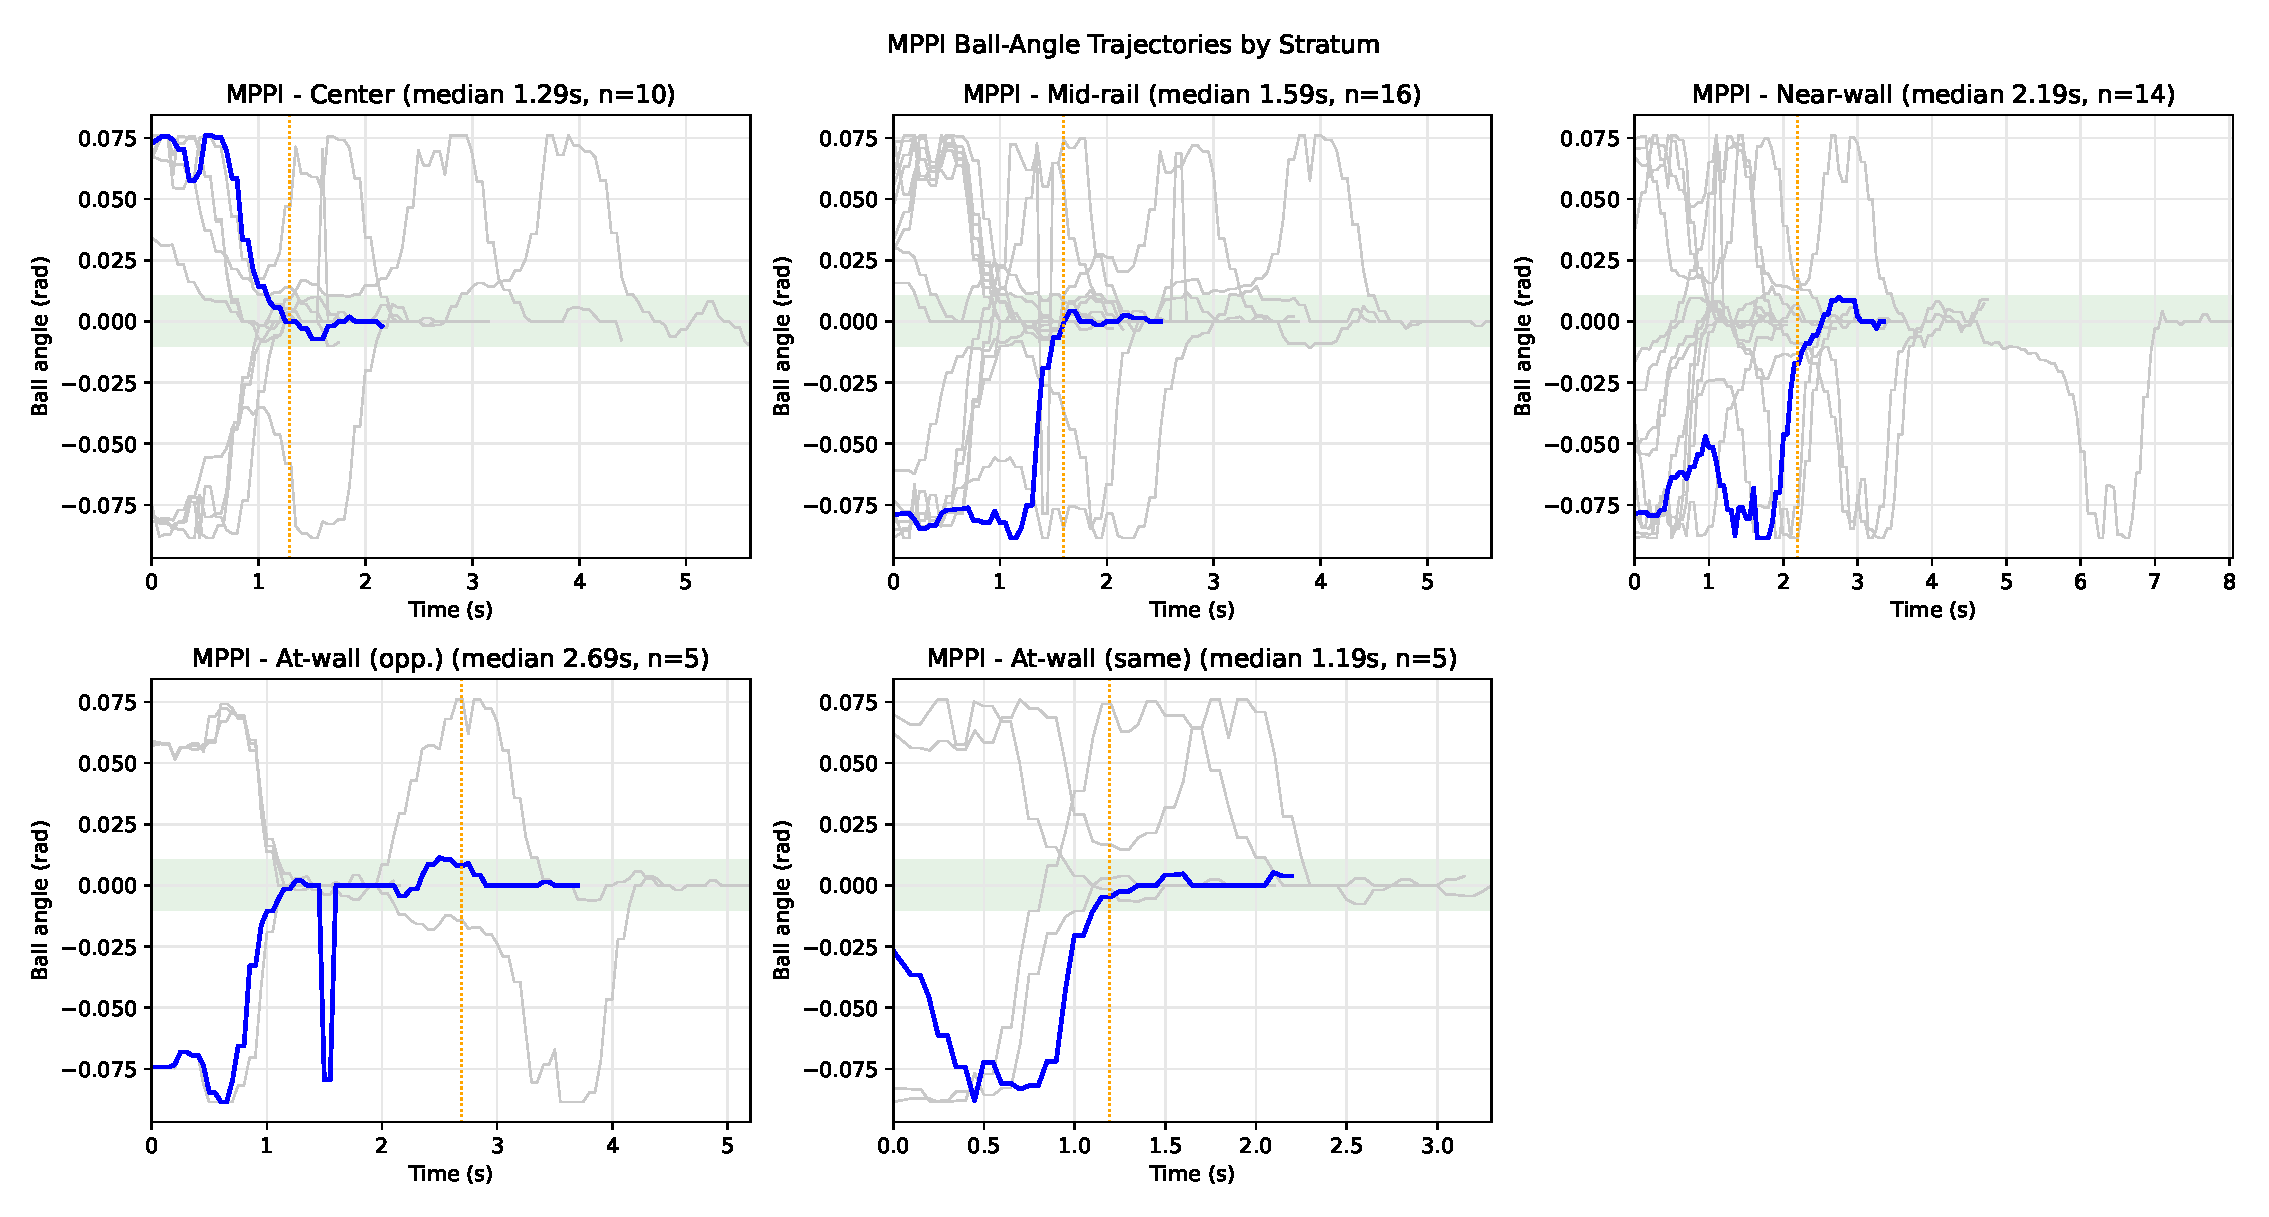
\includegraphics[width=0.95\columnwidth]{figures/mppi_trajectories_by_difficulty.eps}
  \caption{MPPI ball-angle trajectories by stratum. Each panel shows all
    trials in the stratum (gray) with the median-settling trial highlighted
    (blue) and the median settling time marked (dotted). The controller
    settles the ball within the $\pm 0.01$\,rad band (green region) across
    all strata, with median settling from about 1.2\,s (at-wall-same and
    center) to 2.7\,s (at-wall-opposite).}
  \label{fig:mppi_traj_difficulty}
\end{figure}


% ------------------------------------------------------------
% PART III - Experimental Setup
% ------------------------------------------------------------
\section{Dataset Collection Protocol}
\label{appendix:dataset_details}

\noindent\textit{This appendix describes the random-exploration dataset used for world model
training (Appendix~\ref{appendix:world_model}). The 333k post-recalibration dataset used
for IQL training is described in Appendix~\ref{appendix:offline_rl}. The
experimental evaluation protocol (stratified benchmarking) is in
Appendix~\ref{appendix:protocol}.}

\begin{figure}[H]
  \centering
  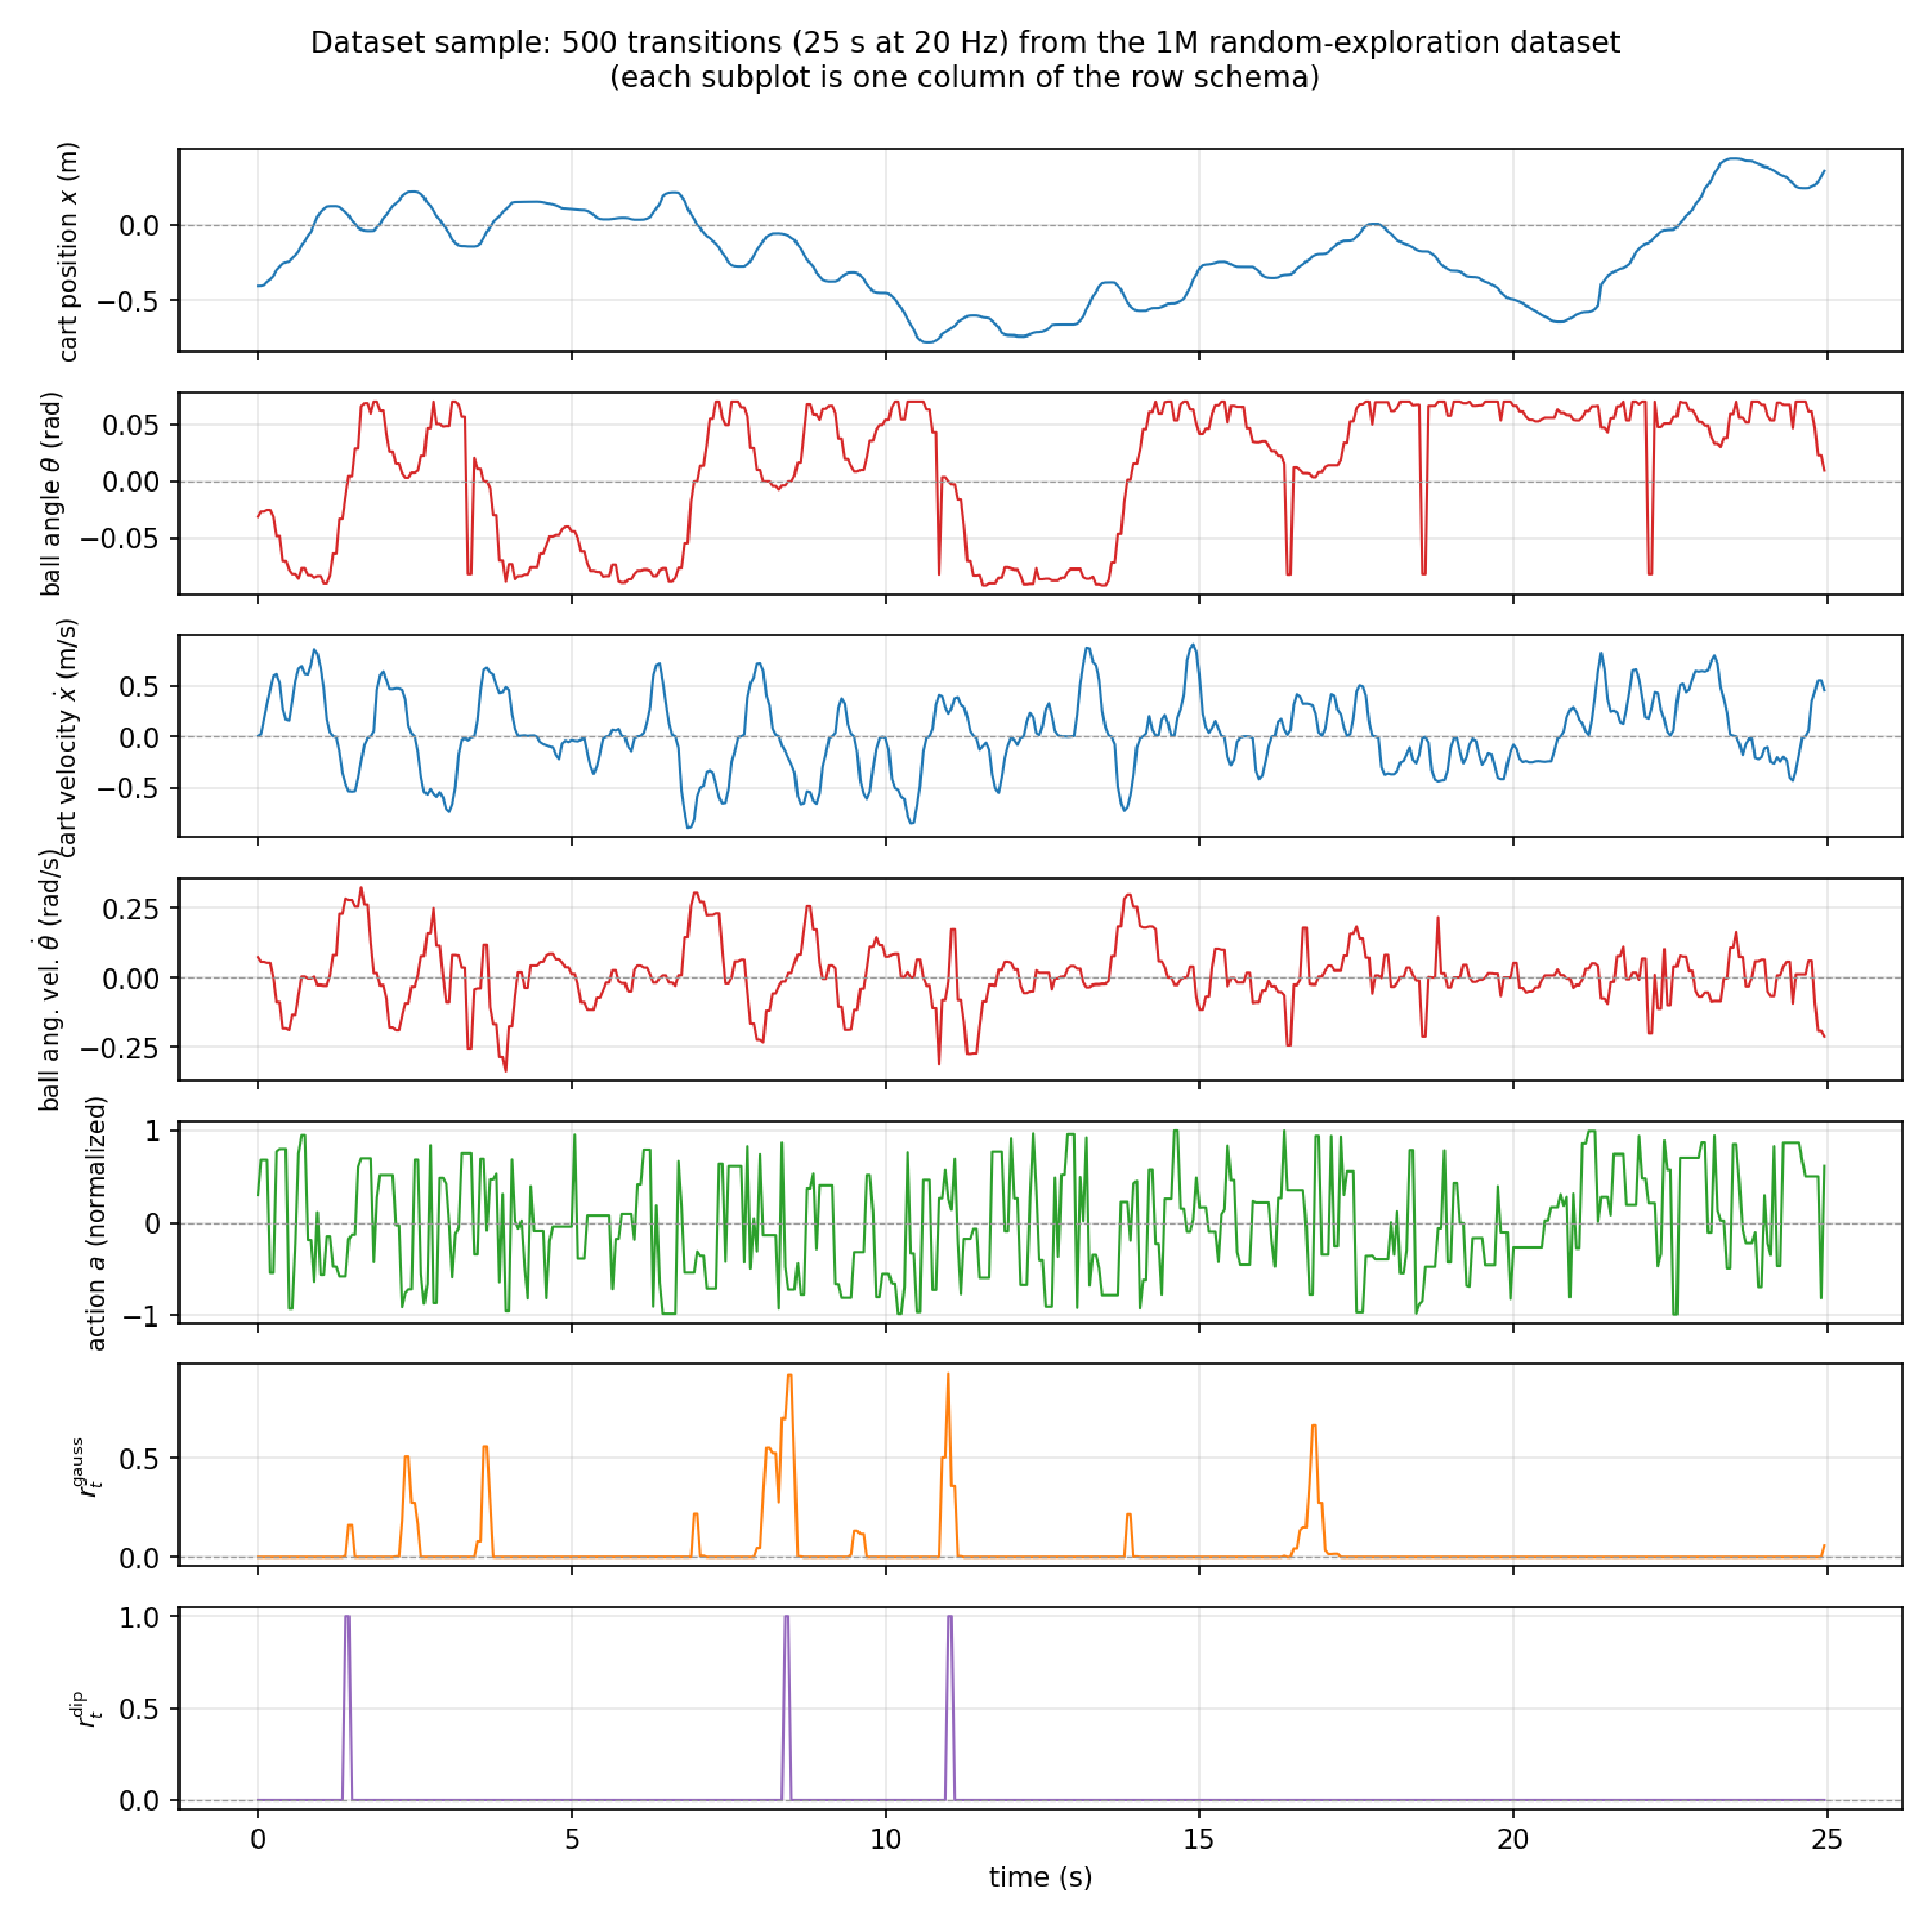
\includegraphics[width=0.98\columnwidth]{figures/dataset_sample.eps}
  \caption{A 500-transition contiguous sample of the 1M
    random-exploration dataset (row schema of
    Eq.~\ref{eq:dataset_row}), plotted as a time series at the 20\,Hz
    control rate. Each subplot is one variable of the row: cart position
    $x$, ball angle $\theta$, cart velocity $\dot{x}$, ball angular
    velocity $\dot{\theta}$, the action $a$ (plotted normalized to
    $[-1,1]$), the Gaussian position reward $r^{\mathrm{gauss}}_t$, and the
    binary IR-dip reward $r^{\mathrm{dip}}_t$ (the hardware IR dip-sensor
    bit, 1 while the sensor reports the ball over the central dip).}
  \label{fig:dataset_sample}
\end{figure}

We recorded random trajectories covering the full state space to
support downstream tasks such as system identification, offline RL,
and learning-based world modeling, collecting separate datasets for
discrete and continuous actions. The agent's normalized action
($\{-1, 0, +1\}$ discrete, $[-1,1]$ continuous) maps to a physical
cart-velocity command ($\{-0.9, 0, +0.9\}$ and $[-0.9, 0.9]$\,m/s). The
stored $a_t$ depends on the collection: the calibrated 1M files store this
m/s command, while the earlier \texttt{pre\_neg} collection stores the
normalized action in $[-1,1]$.
Each row contains:
\begin{equation}
\label{eq:dataset_row}
[x_t,\, \dot{x}_t,\, \theta_t,\, \dot{\theta}_t,\; a_t,\;
 x_{t+1},\, \dot{x}_{t+1},\, \theta_{t+1},\, \dot{\theta}_{t+1},\;
 r^\text{gauss}_t,\; r^\text{dip}_t],
\end{equation}
where
\begin{align}
r^\text{gauss}_t &=
  \exp\!\Bigl(-\frac{\theta_t^2}{2\sigma_r^2}\Bigr)
  \cdot
  \exp\!\Bigl(-\frac{|\dot{\theta}_t|}{v_\text{scale}}\Bigr),
\\
r^\text{dip}_t &=
\begin{cases}
1, & |\theta_{t+1}| \le \theta_\text{center} \\
0, & \text{otherwise.}
\end{cases}
\end{align}
Here $\sigma_r = \theta_\text{max}/16 \approx 0.005$\,rad sets the width
of the Gaussian position reward ($\theta_\text{max}$ is the ball angular
limit, 0.081\,rad in the calibrated collections and 0.075 in
\texttt{pre\_neg}), $v_\text{scale} = 0.2$\,rad/s scales the
angular-velocity term, and $\theta_\text{center} = 0.007$\,rad
(about 15\,mm of arc at $R = 2.101$\,m) is the dip half-band. In the 1M
random-exploration files, the stored $r^\text{dip}_t$ column is the raw
hardware IR dip-sensor bit read from the serial stream; the angular form
above, evaluated on the next-state angle $\theta_{t+1}$, is the offline
recomputation applied when rebuilding the 333k post-recalibration dataset
(\texttt{build\_flat\_dataset.py}).
We recorded over one million steps for the random-exploration
dataset used for world model training, stored in compressed HDF5
format, with the full acquisition scripts available in the public
repository. The two released 1M collections differ in layout: the
calibrated files (\texttt{calib196\_148}, \texttt{calib196\_160}) add four
raw time-of-flight columns (previous and current \texttt{raw\_left\_mm} and
\texttt{raw\_right\_mm}) for a 15-column on-disk array, while the earlier
\texttt{pre\_neg} collection is the 11-column form of
Eq.~\ref{eq:dataset_row}. The world-model loader reads only the
four-element state, the action, and the four-element next state.

Figure~\ref{fig:dataset_sample} shows a 500-transition contiguous
sample from the 1M random-exploration dataset, one subplot per variable
in the row schema of Eq.~\ref{eq:dataset_row}, giving a visual sense of
what one dataset ``looks like'' as a time series (the caption details
each channel).

We used the 1M-transition random-exploration dataset
exclusively to train the LSTM world model
(Appendix~\ref{appendix:world_model}),
which is then used by MPPI and PPO-WM (two checkpoints trained on
two 1\,M collections; see Appendix~\ref{appendix:wm_provenance}). It is \emph{not} used
for offline RL training, because random actions provide insufficient
coverage of successful recovery behavior for an offline policy.
IQL instead uses a separate post-recalibration dataset (333{,}497
transitions from 1{,}415 mixed-controller hardware trials, rewards
recomputed offline), detailed in Appendix~\ref{appendix:offline_rl}. It
is available as \texttt{arcball\_post\_recalib\_flat.h5} (built by
\texttt{data/build\_flat\_dataset.py}).

\subsection{Data-Collection Notes}
\label{appendix:dataset_notes}

Two practical lessons from collecting these datasets on real hardware are
worth recording, since both bear directly on data quality downstream.

\textbf{Solder the sensor wiring:} connect the time-of-flight sensors to the
Arduino with soldered joints rather than push-fit jumper or breadboard
connections. During random exploration the ball strikes the arc walls
repeatedly, and the resulting vibration gradually loosens push-fit
connectors. A momentarily broken power or signal line produces dropped or
frozen readings that are easy to miss during a long unattended collection
run; a soldered harness removes this failure mode.

\textbf{Inspect trajectories before training:} visualize the recorded state
variables before committing a dataset to training. A sensor channel can go
dead partway through a run and hold a constant or otherwise invalid value
that still passes the on-line validity checks, so the fault survives into
the stored data. Plotting each state variable as a time series (as in
Figure~\ref{fig:dataset_sample}) makes such segments immediately visible;
training on them silently degrades the world model and any policy learned
downstream.

\section{Evaluation Protocol}
\label{appendix:protocol}


\subsection{Initial Conditions and Success Criteria}
\label{sec:ic_design}

\textbf{Hardware trials.}
We use a stratified initial condition (IC) design to ensure
fair comparison across controllers with different constraint-handling
capabilities. Strata are defined mainly by the cart's starting
position (available maneuvering space), and at the rail by the targeted
ball side. The cart is positioned automatically via closed-loop
velocity control (P-controller, 10~mm tolerance), and the ball is
displaced from center via brief cart jolts.

The 50-trial schedule comprises five strata:
\begin{itemize}
    \item \textbf{Center (20\%, 10 trials):} Cart at $\pm 0.10$~m,
          ball jolted off center.
    \item \textbf{Mid-rail (32\%, 16 trials):} Cart at $\pm 0.40$~m,
          ball jolted off center. Tests recovery
          with asymmetric rail budget ($\sim$0.38~m one side,
          $\sim$1.18~m other).
    \item \textbf{Near-wall (28\%, 14 trials):} Cart at $\pm 0.65$~m,
          ball jolted off center. Tests recovery
          under tight constraints (only 0.13~m clearance on one side).
    \item \textbf{At-wall-opposite (10\%, 5 trials):} Cart at
          $\pm 0.78$~m (workspace limit, axis units), ball displaced to
          \emph{opposite} side. Feasible for all controllers;
          tests recovery speed.
    \item \textbf{At-wall-same (10\%, 5 trials):} Cart at
          $\pm 0.78$~m (workspace limit, axis units), ball displaced to
          \emph{same} side as cart. Reveals structural limitations
          of controllers without explicit constraint handling.
\end{itemize}

Trials alternate left/right within each stratum and are shuffled
deterministically (seed~42) so every controller sees the identical
sequence.  The schedule is logged alongside results for reproducibility.

Beyond the ball-side selection in the two at-wall strata, the ball's
initial angle $\theta_0$ is not controlled: it arises from
the brief cart jolt used to displace the ball. Empirically,
$\theta_0 \in [-0.091, 0.081]$~rad across the benchmark trials
(mean $|\theta_0| \approx 0.062$~rad, standard deviation $\approx 0.019$~rad),
and it stays in the same range in every stratum, with per-stratum mean
$|\theta_0|$ ranging only from $0.059$~rad (at-wall-opposite) to $0.071$~rad
(at-wall-same). The initial ball displacement is therefore comparable across
strata, so stratum difficulty reflects maneuvering room rather than initial
ball displacement.

The jolt also places the ball outside the central dip in nearly every trial.
With the surface parameters of Section~\ref{appendix:dynamics}, the dip's
restoring region reaches only to $|\theta| \approx 0.0115$~rad. Released at rest
inside that angle with the cart held still, the ball returns to center, and
released outside it, the ball rolls away down the convex arc. All but five of the 650 benchmark trials start beyond that angle, at a
mean $|\theta_0|$ some five times larger, so a controller has to carry the ball
back across the destabilizing part of the arc before the dip can capture it.

One caveat applies to the achieved cart start in the at-wall strata, where the
cart is driven toward the rail ($|x_0| = 0.777$~m) before the ball is displaced.
In the at-wall-\emph{same} stratum the cart reached the physical limit on about
$83\%$ of the 13 benchmark controllers' trials, but this was not uniform across
controllers: most reached the rail on all five trials, whereas for a few,
notably NMPC and TD3, on three of their five trials the automated placement
left the cart near center ($|x_0| \approx 0.08$~m) rather than at the rail, a
materially easier start. Both still succeeded on all five, and within this stratum the
success rate does not differ significantly between trials that reached the limit
and those that did not ($50/54$ versus $9/11$; Fisher's exact test $p = 0.27$),
so the effect on the reported comparison is small. The at-wall-\emph{opposite}
stratum is less uniform still: the cart reached the limit for only some
controllers and started nearer center ($|x_0| \approx 0.09$~m) for the others.
We therefore read both at-wall strata as recovery-speed checks for the
controllers that did not reach the rail, rather than strictly equal-condition
cross-controller robustness comparisons.

\textbf{Simulation controller benchmarks} (the RL and classical
comparisons run in simulation) use the same 50-trial stratified schedule
as the hardware protocol (cart at
$\pm 0.10, \pm 0.40, \pm 0.65, \pm 0.78$~m). The simulator also provides a
legacy uniform-sampling mode,
\begin{align}
  x_0 &\sim \mathcal{U}(-0.75,\;0.75)~\text{m}, \nonumber\\
  \theta_0 &\sim \mathcal{U}(-0.074,\;0.074)~\text{rad}, \nonumber\\
  \dot{x}_0 &= \dot{\theta}_0 = 0,
\end{align}
but it was not used for the reported benchmarks.

\textbf{Success criterion.}
A trial is \textbf{successful} if the ball angle satisfies
\begin{equation}
  |\theta(t)| < 0.01~\text{rad}
\end{equation}
\emph{continuously} for at least $1.0$~s.
The \textbf{settling time} $t_s$ is defined as the wall-clock time at
which the ball \emph{enters} this band and remains within it for the
required duration (i.e.\ the entry instant, not the end of the window).
The maximum trial duration is $30$~s; trials not meeting the settling
criterion within this window are recorded as failures.

\subsection{Performance Metrics}

We evaluate controllers using the following metrics, computed with
SciPy~\cite{2020SciPy-NMeth} and NumPy~\cite{harris2020array}:

\begin{itemize}
    \item \textbf{Settling time} ($t_s$): wall-clock time from trial start
    until the success criterion is first met (as defined above). Medians,
    interquartile ranges, and the settling significance tests are computed
    over \emph{successful trials only}, matching the main paper's Table~II
    statistics; success rate is reported separately, so reliability is not
    folded into the settling comparison.

    \item \textbf{Success rate}: fraction of trials with $t_s < 30.0$~s,
    with 95\% Wilson score intervals. Wilson intervals replace a bootstrap
    because a perfect $50/50$ record bootstraps to a degenerate
    $[100, 100]$ interval, understating uncertainty at the boundary.

    \item \textbf{Control effort}: root-mean-square commanded cart
    velocity in m/s, saturated at the $\pm 0.9$~m/s axis limit the
    actuator enforces, computed per trial and averaged over all trials.

    \item \textbf{Significance testing.}
    Pairwise Mann-Whitney $U$ rank tests
    (\texttt{scipy.stats.mannwhitneyu}) on the successful-trial
    settling distributions, Bonferroni-corrected~\cite{bonferroni1936teoria}
    across all $\binom{13}{2}=78$ pairs ($\alpha_c = 0.05/78$). A rank test
    is used because the settling distributions are right-skewed, so a
    mean-based $t$-test is inappropriate. Success-rate differences use
    Fisher's exact test (\texttt{scipy.stats.fisher\_exact}) over the same
    family. Control-effort differences are tested the same way, as a separate
Mann-Whitney family over the per-trial RMS effort across all $78$ pairs, with
the full pairwise matrix written to \texttt{exp1\_effort\_significance.csv}.
Effect sizes are reported as Cohen's $d$
    ($d = (\bar{x}_i - \bar{x}_j)/s_{\mathrm{pooled}}$,
    $s_{\mathrm{pooled}} = \sqrt{(s_i^2 + s_j^2)/2}$, equal-weight pooling)
    to complement the $p$-values. Because the 78 pairwise tests are computed
    on overlapping controller data rather than independent samples, the
    Bonferroni correction is conservative here, so the number of pairs flagged
    significant is best read as a lower bound. All statistics are reproduced by
    \texttt{paper/scripts/compute\_statistics.py}.
\end{itemize}

\subsection{Experiment 1: Baseline Performance}

\paragraph{Objective:}
Establish the nominal performance hierarchy under realistic but
unperturbed sensing conditions, using difficulty-stratified ICs that
test regulation, recovery, and constraint handling.

\paragraph{Protocol:}
We evaluate each controller over 50 trials on the physical
platform at the nominal control frequency of 20~Hz
($T_s = 0.05$~s).
Sensor readings use the 34.5~ms timing-budget sequential ToF
configuration (Appendix~\ref{appendix:sensor_characterization}) with inherent noise
($\sigma_{\text{ToF}} \approx 1.6$--$1.7$~mm at the arc center);
no additional artificial noise is injected.

\paragraph{Rationale:}
The stratified IC design ensures that:
(a) no controller is unfairly penalized by impossible starting
conditions;
(b) center strata establish baseline regulation performance;
(c) near-wall/at-wall strata discriminate controllers by their
constraint-handling and recovery capabilities;
(d) the identical IC sequence across all controllers removes
IC-related confounds from pairwise comparisons, with the exception of
the achieved cart start in the two at-wall strata, which was not uniform
across controllers (Section~\ref{sec:ic_design}).


% ------------------------------------------------------------
% PART IV - Results
% ------------------------------------------------------------
\section{Simulation Validation}
\label{appendix:simulation_validation}

\noindent\textit{This appendix validates that the two dynamics models used by
controllers in the main paper, the analytical first-principles model and the
learned LSTM world model, are accurate enough predictors of real hardware
dynamics.  Rather than comparing controller-level metrics (success rate,
settling time), we evaluate open-loop trajectory prediction accuracy against
held-out partitions of the 1\,M-transition real dataset.  This isolates model error from
controller behavior and provides a direct measure of simulation fidelity.}

\subsection{Methodology}
\label{sec:sim_val_method}

We follow a standard open-loop prediction protocol:
\begin{enumerate}
  \item From a dataset of real hardware transitions
        $(\mathbf{s}_t, a_t, \mathbf{s}_{t+1})$, select $N$ reset-free
        segments of length $L$.
  \item For each segment, initialize a candidate model to the real state
        $\mathbf{s}_0$ and replay the recorded action sequence
        $a_0, a_1, \dots, a_{L-1}$ open-loop.
  \item Record the predicted trajectory
        $\hat{\mathbf{s}}_1, \dots, \hat{\mathbf{s}}_L$ and compute
        terminal MAE $|\hat{\mathbf{s}}_L - \mathbf{s}_L|$ and
        trajectory MAE $\frac{1}{L}\sum_{t=1}^{L} |\hat{\mathbf{s}}_t - \mathbf{s}_t|$.
  \item Report means across all segments.
\end{enumerate}

\paragraph{Metric choice.}
We report mean absolute error (MAE) rather than root-mean-square error (RMSE)
because MAE is robust to outliers and directly interpretable in physical units.
Since the four state variables operate on very different scales (cart position
$\pm 0.78$\,m, ball angle $\pm 0.081$\,rad), we also report \emph{normalized MAE}
(MAE divided by the variable's full operating range, expressed as a percentage).
Normalized MAE makes channels comparable and reveals which state dimensions
are predicted most poorly relative to their dynamics.

We use two configurations:
\begin{itemize}
  \item \textbf{Exp 1 (short horizon):} $N=100$ segments, filtered to
        initial conditions (IC) with $|\theta| < 0.04$\,rad
        (ball near center), horizons $0.25$--$2.5$\,s ($5$--$50$ steps).
        This corresponds to the prediction horizon used by model-based
        controllers (MPPI, NMPC).
  \item \textbf{Exp 2 (long horizon):} $N=50$ segments with no IC filter,
        horizons $0.25$--$30$\,s ($5$--$600$ steps).
        This covers the episode length used by RL agents.
\end{itemize}

Under the 80/10/10 split used to train the world model, the analytical
ablation (Exp 1, which selects the best analytical configuration) draws
segments from the validation partition (rows 80--90\%), and the
world-model comparison (Exp 2) draws from the held-out test partition
(rows 90--100\%). Neither partition receives gradient updates; the
validation partition (Exp 1) is used only for early stopping and
checkpoint selection, while the test partition (Exp 2) is fully held out
and drives the primary world-model comparison. Both slices are disjoint
from the one used to pick the analytical configuration.

The candidate models are:
\begin{itemize}
  \item \textbf{Analytical model}: the velocity-input first-principles model
        (Section~\ref{sec:velocity_input}) with nominal parameters
        ($\tau_v = 0.15$\,s, $d = 0.002$\,m, $\mu_\mathrm{rr} = 0.025$,
        $\beta_v = 0.009$~m$^2$/s), Euler integration with step size
        0.05\,s, a 1-step command delay, and a first-order velocity
        observation filter (PT1, $\tau = 10$~ms).
        Additional structural variants are compared in the ablation below.
  \item \textbf{World model}: a 2-layer LSTM (hidden dim~64, sequence
        length~10) trained on 1\,M real transitions, as detailed in
        Appendix~\ref{appendix:world_model}.  It predicts the state delta
        $\Delta\mathbf{s}_{t+1}$ with a skip connection.  During rollout
        the LSTM hidden state is maintained across steps to capture
        temporal dynamics.
\end{itemize}

\subsection{Analytical Model Ablation}
\label{sec:sim_val_ablation}

Before comparing against the world model, we ablate the analytical model
to quantify the contribution of each pipeline component.  All ablations
are at $h=50$ ($2.5$\,s).

\paragraph{Pipeline components.}
Figure~\ref{fig:sim_val_waterfall_pipeline} shows the cumulative effect
of adding each pipeline element.  The bare model ($\tau_v = 0.06$, no
delay, no filter) has a total trajectory MAE (sum over 4 channels)
of 0.756.  Calibrating $\tau_v$ to 0.15 reduces this to 0.521, a 31\%
improvement that accounts for the majority of the total gain.  Adding
a discrete one-step (50\,ms) command-delay approximation
further reduces error to 0.476. The 50\,ms one-step delay is a
conservative upper bound on the measured real transport delay (under
14\,ms) and is retained in the training and tuning simulators
(Appendices~\ref{appendix:rl_training} and~\ref{appendix:tuning_insights}).  The velocity observation filter (PT1,
$\tau = 10$\,ms) adds a small additional improvement to 0.444.

\begin{figure}[!tbp]
  \centering
  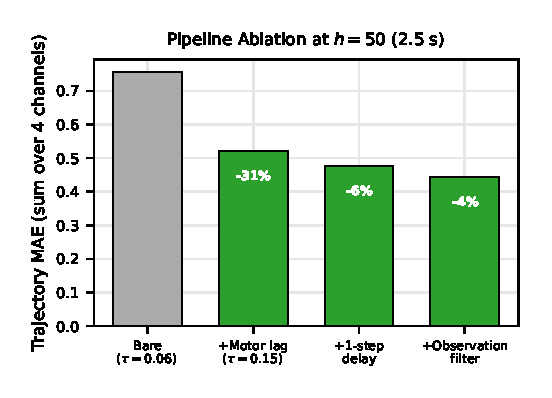
\includegraphics[width=\columnwidth]{figures/sim_val_waterfall_pipeline.eps}
  \caption{Pipeline ablation: total trajectory MAE (sum of 4 channels)
           at $h=50$ ($2.5$\,s).  Calibrating $\tau_v$ accounts for the
           largest improvement; command delay and observation filtering
           provide diminishing returns.}
  \label{fig:sim_val_waterfall_pipeline}
\end{figure}

The normalized MAE (Table~\ref{tab:sim_val_ablation}) shows that ball
angle $\theta$ has the highest relative error (33\% of operating range
even with the bare model), confirming that the ball dynamics are the
hardest channel to predict regardless of modeling choices.

\begin{table*}[!t]
\centering
\caption{Pipeline ablation: normalized trajectory MAE (\% of operating range)
         at $h=50$ ($2.5$\,s).  Raw MAE values in parentheses.}
\label{tab:sim_val_ablation}
\begin{tabular}{lcccc}
\toprule
Variant & $x$ & $\dot{x}$ & $\theta$ & $\dot{\theta}$ \\
\midrule
Bare ($\tau_v = 0.06$)
  & 6\%\,(0.099)  & 23\%\,(0.417)  & 33\%\,(0.054) & 19\%\,(0.186) \\
$+\tau_v = 0.15$
  & 5\%\,(0.084)  & 15\%\,(0.267)  & 28\%\,(0.046) & 12\%\,(0.124) \\
$+$Delay (1 step)
  & 5\%\,(0.082)  & 13\%\,(0.226)  & 30\%\,(0.048) & 12\%\,(0.120) \\
$+$Obs filter
  & 5\%\,(0.082)  & 12\%\,(0.208)  & 29\%\,(0.047) & 11\%\,(0.108) \\
\bottomrule
\end{tabular}
\end{table*}

\paragraph{Best analytical configuration.}
Based on this ablation, the best analytical model is: velocity-input
first-principles ball dynamics, first-order velocity lag
($\tau_v = 0.15$\,s), 1-step command delay, and velocity observation
filter (PT1, $\tau = 10$\,ms).  This configuration is used as the
``analytical model'' in the remainder of this appendix and in all
controllers that rely on the analytical simulator.

\subsection{Analytical Model vs.~World Model}
\label{sec:sim_val_comparison}

We now compare the best analytical model against the LSTM world model.
Table~\ref{tab:sim_val_comparison} reports terminal MAE as a percentage
of each channel's operating range.

\begin{table*}[!t]
\centering
\caption{Terminal MAE (\% of operating range) at representative horizons.
         Negative $\Delta$ indicates world model improvement.}
\label{tab:sim_val_comparison}
\begin{tabular}{llccccc}
\toprule
Horizon & Model & $x$ (\%) & $\dot{x}$ (\%) & $\theta$ (\%) & $\dot{\theta}$ (\%) & Avg. (\%) \\
\midrule
\multirow{3}{*}{0.25\,s}
  & Analytical  & 2 & 13 & 11 & 11 & 9 \\
  & World Model & 2 &  9 &  7 &  5 & 6 \\
  & $\Delta$    & $+4$\% & $-34$\% & $-34$\% & $-55$\% & \\
\addlinespace
\multirow{3}{*}{2.5\,s}
  & Analytical  & 8 & 12 & 31 & 10 & 15 \\
  & World Model & 9 &  7 & 40 &  6 & 16 \\
  & $\Delta$    & $+2$\% & $-46$\% & $+30$\% & $-37$\% & \\
\addlinespace
\multirow{3}{*}{10.0\,s}
  & Analytical  & 11 & 15 & 38 & 12 & 19 \\
  & World Model & 10 &  5 & 36 &  7 & 15 \\
  & $\Delta$    & $-10$\% & $-70$\% & $-6$\% & $-45$\% & \\
\addlinespace
\multirow{3}{*}{30.0\,s}
  & Analytical  & 20 & 14 & 42 &  8 & 21 \\
  & World Model & 15 &  4 & 42 &  8 & 17 \\
  & $\Delta$    & $-28$\% & $-70$\% & $-1$\% & $+8$\% & \\
\bottomrule
\end{tabular}
\end{table*}

Figure~\ref{fig:sim_val_error_growth} visualizes the full error growth
curves.

\begin{figure*}[!tbp]
  \centering
  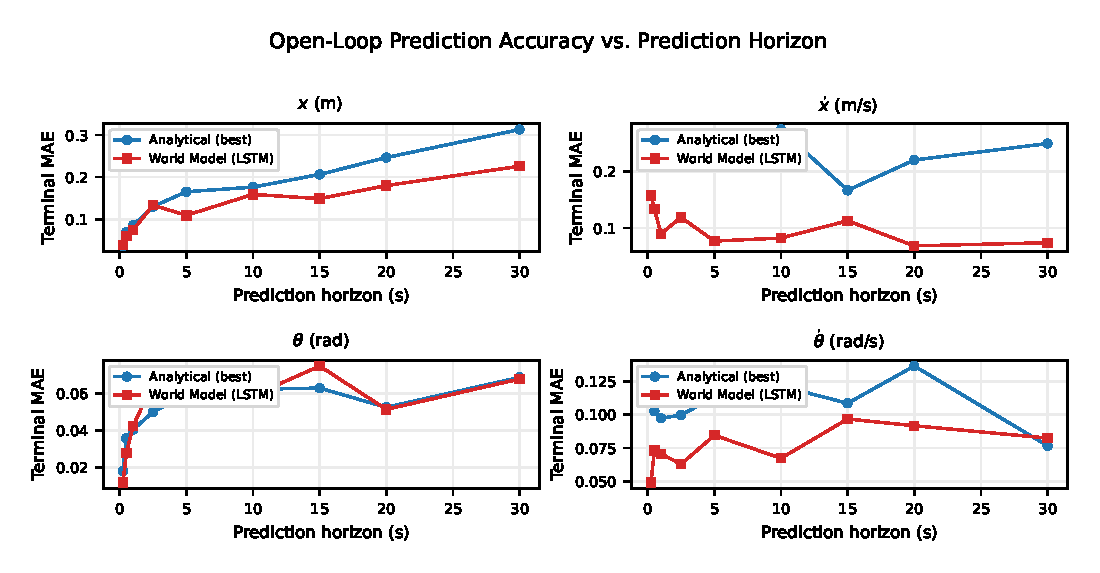
\includegraphics[width=\textwidth]{figures/sim_val_error_growth.eps}
  \caption{Terminal MAE vs.~prediction horizon for the analytical model
           (blue) and world model (red), one panel per state channel.
           The world model has lower terminal MAE at most horizons on cart
           position and both velocities; the exception is terminal ball-angle
           error, where the analytical model matches or beats it at 1, 2.5,
           5, and 15\,s.
           Error growth is sub-linear for both models,
           indicating no catastrophic divergence.}
  \label{fig:sim_val_error_growth}
\end{figure*}

\paragraph{Normalized perspective.}
Normalized MAE reveals that the analytical model's weakest channel is
ball angle $\theta$: at 2.5\,s it reaches 31\% of the ball's total
range, and at 30\,s it reaches 42\%.  Cart position and velocity stay
below about 20\% even at the longest horizon.  This asymmetry reflects the
indirect coupling: $\theta$ is driven through the arc geometry, which
amplifies residual error from the cart model.

The world model's advantage is largest on cart velocity
($\dot{x}$ improves by 34--70\% across the horizons). For ball angle
$\theta$ the two models are close, and the world model is actually worse
at 2.5\,s ($+30$\%). This is because ball angle is primarily determined by the
physical geometry and gravity, dynamics that both models capture
equally well, while velocity dynamics are more sensitive to the
unmodeled servo behavior that the LSTM learns.

\subsection{Crossover Analysis}
\label{sec:sim_val_crossover}

A key question is whether there exists a prediction horizon at which
the simpler analytical model matches or beats the learned world model,
i.e., a \emph{crossover}.  Figure~\ref{fig:sim_val_crossover} shows
the ratio of world model to analytical total trajectory MAE across
all horizons.

\begin{figure}[!tbp]
  \centering
  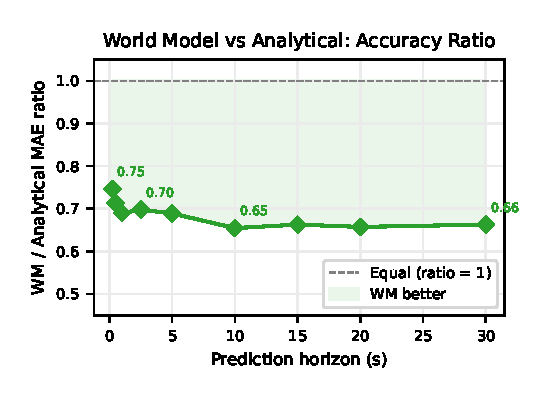
\includegraphics[width=\columnwidth]{figures/sim_val_crossover_ratio.eps}
  \caption{Ratio of world model to analytical total MAE vs.~prediction
           horizon.  Values below~1 indicate the world model is more
           accurate.  The world model wins at every horizon on total error; no crossover
           exists.  The ratio stays between about 0.65 and 0.75
           (25--35\% lower error), with the smallest margin at 0.25\,s and
           the largest around 10\,s.}
  \label{fig:sim_val_crossover}
\end{figure}

\paragraph{Crossover across horizons.}
The world model has lower total trajectory MAE across all tested
horizons ($0.25$--$30$\,s), by between 25 and 35\%: it is 25\% lower at
0.25\,s, peaks near 35\% around 10\,s, and holds about 34\% out to 30\,s.
There is no regime where the analytical model catches up on total error. These are point estimates from a single
evaluation run (100 segments in Exp 1, 50 in Exp 2); per-segment
dispersion, confidence intervals, and paired significance tests are not
reported, so the ordering is descriptive rather than statistically tested.

\paragraph{Implication for controller selection.}
For sampling-based predictive controllers that roll out many candidate
trajectories through the model (e.g.~MPPI with $H = 30$, a 1.5\,s
lookahead), the world model provides the largest relative benefit,
because every sampled trajectory inherits the model's higher fidelity
over the full rollout.  For classical and predictive controllers designed
around the analytical model (LQR+WO, MPC+WO, NMPC, SMC+WO), the analytical
model is sufficient: its short-horizon accuracy (0.018\,rad at
0.25\,s, 11\% of range) is adequate for feedback correction, and
closed-loop control compensates for residual model error.
For model-free RL trained purely in simulation (PPO~(BZ+DR), SAC~(DR),
TD3~(DR), TQC~(DR), TRPO~(DR)), the analytical model is likewise
sufficient because domain randomization and the controller's own
robustness absorb the
prediction gap, as confirmed by the hardware success rates in the
main paper.

The world model provides its largest benefit in two settings: (i)~zero-shot
deployment of PPO-WM, which achieves 100\% hardware success rate without
domain randomization, and (ii)~real-time trajectory optimization in MPPI,
where the learned model's higher fidelity directly improves sampled
trajectory quality relative to the analytical model.

\subsection{Summary}

\begin{enumerate}
  \item \textbf{Pipeline components contribute unequally.} Calibrating
        $\tau_v$ accounts for the largest improvement.  Command delay
        and observation filtering provide diminishing returns.
  \item \textbf{Ball angle is the hardest channel.} Normalized MAE for
        $\theta$ reaches 31\% of range at 2.5\,s (analytical model),
        compared to 8--12\% for the other channels.
  \item \textbf{World model has lower trajectory-mean error.} Its total
        trajectory MAE is 25--35\% lower than the analytical model's at
        every horizon (the analytical model is about 1.3--1.5$\times$
        higher), with the largest advantage on cart velocity ($\dot{x}$).
        Terminal ball-angle error is mixed: the analytical model matches
        or beats the world model at 1, 2.5, 5, and 15\,s.
  \item \textbf{Analytical model is sufficient for its use cases.}
        Classical, predictive, and domain-randomized RL controllers reach
        high hardware success with the analytical model, which suggests
        closed-loop feedback and domain randomization absorb the residual
        prediction error. This is an inference from open-loop prediction
        accuracy and the measured hardware success rates, not a controlled
        controller-level swap of the dynamics model.
  \item \textbf{World model delivers its largest gains where fidelity
        matters most.} Higher prediction fidelity most benefits
        world-model-based RL (PPO-WM at 100\% SR) and MPPI trajectory
        optimization.
\end{enumerate}

\section{Detailed Statistics and Per-Trial Data}
\label{appendix:per_trial}

\noindent\textit{This appendix provides per-stratum breakdowns and detailed statistics
for individual controllers. The full 13-controller benchmark results
(Table~II equivalent) are given in Table~\ref{tab:full_results} below.}

\subsection{MPPI: Per-Stratum Breakdown (50 Trials)}

\begin{table}[t]
\centering
\caption{MPPI hardware results by stratum.}
\begin{tabular}{lccccc}
\toprule
\textbf{Difficulty} & \textbf{Trials} & \textbf{SR} & \textbf{Mean (s)} & \textbf{Med (s)} & \textbf{Max (s)} \\
\midrule
Center & 10 & 100\% & 1.82 & 1.29 & 4.59 \\
Mid-rail & 16 & 100\% & 1.99 & 1.59 & 4.59 \\
Near-wall & 14 & 100\% & 2.33 & 2.19 & 7.04 \\
At-wall-opposite & 5 & 100\% & 2.52 & 2.69 & 4.19 \\
At-wall-same & 5 & 100\% & 1.56 & 1.19 & 2.34 \\
\midrule
\textbf{Overall} & \textbf{50} & \textbf{100\%} & \textbf{2.06} & \textbf{1.67} & \textbf{7.04} \\
\bottomrule
\end{tabular}
\end{table}

MPPI's median settling varies little across strata: it barely
moves with the starting position, from 1.19\,s at at-wall-same and 1.29\,s at
center to 2.69\,s at at-wall-opposite, a spread of only about 1.5\,s despite
the very different maneuvering room.

\subsection{Complete Benchmark Results (All 13 Controllers)}

Table~\ref{tab:full_results} reports the definitive 50-trial hardware
benchmark for all 13 deployed controllers, sorted by hardware success
rate then by mean settling time (the same controllers as Table~II of the main
paper, extended here with the bootstrap settling-time confidence band and
mean per-step compute time). SR 95\% confidence intervals are Wilson
score intervals (matching Appendix~\ref{appendix:protocol} and the main paper);
settling 95\% confidence intervals are bootstrap over the successful
trials only, and the per-step compute time excludes sensor I/O. Two controllers (MPPI, PPO~(WM)) reach
100\% SR; PPO~(BZ+DR) and PD+WO reach 96\%; the rest span
80--92\%. The classical feedback laws, MPC+WO, and the on-policy RL policies PPO~(BZ+DR) and TRPO~(DR) run in under 1\,ms; IQL, NMPC, PPO-WM, and the off-policy RL policies
(TD3, TQC, SAC) sit in the 2--8\,ms range; and only MPPI ($\sim$40\,ms)
approaches the 50\,ms deadline.

\begin{table*}[t]
\centering
\caption{Complete hardware benchmark: 50 trials per controller, 20\,Hz,
stratified initial conditions. SR intervals are 95\% Wilson score intervals; settling intervals are 95\% bootstrap.}
\label{tab:full_results}
\begin{tabular}{llcccccc}
\toprule
\textbf{Controller} & \textbf{Paradigm} & \textbf{SR (\%)} & \textbf{SR 95\% CI}
  & \textbf{Settle (s)} & \textbf{Settle 95\% CI} & \textbf{RMS Effort}
  & \textbf{Compute (ms)} \\
\midrule
MPPI & Real-data & 100 & [93, 100] & 2.06 & [1.71, 2.44] & 0.354 & 40.0 \\
PPO (WM) & Real-data & 100 & [93, 100] & 6.84 & [5.07, 8.95] & 0.492 & 6.7 \\
PPO (BZ+DR) & Sim-trained RL & 96 & [87, 99] & 3.81 & [2.93, 4.78] & 0.498 & 0.59 \\
PD+WO & Classical & 96 & [87, 99] & 5.80 & [4.08, 7.76] & 0.580 & 0.05 \\
SMC+WO & Classical & 92 & [81, 97] & 8.93 & [7.33, 10.64] & 0.562 & 0.06 \\
LQR+WO & Classical & 92 & [81, 97] & 10.21 & [7.76, 12.79] & 0.625 & 0.33 \\
IQL & Real-data & 92 & [81, 97] & 10.62 & [8.54, 12.76] & 0.395 & 2.0 \\
TD3 (DR) & Sim-trained RL & 92 & [81, 97] & 11.45 & [9.16, 13.87] & 0.680 & 7.9 \\
NMPC & Predictive & 90 & [79, 96] & 7.48 & [5.19, 10.08] & 0.608 & 5.7 \\
TRPO (DR) & Sim-trained RL & 90 & [79, 96] & 8.09 & [6.01, 10.43] & 0.508 & 0.67 \\
TQC (DR) & Sim-trained RL & 86 & [74, 93] & 9.77 & [7.25, 12.39] & 0.663 & 7.9 \\
SAC (DR) & Sim-trained RL & 82 & [69, 90] & 10.10 & [7.80, 12.42] & 0.588 & 7.8 \\
MPC+WO & Predictive & 80 & [67, 89] & 10.81 & [8.04, 13.55] & 0.623 & 0.47 \\
\bottomrule
\end{tabular}
\end{table*}

\begin{figure}[t]
  \centering
  
\includegraphics[width=0.95\columnwidth]{figures/hw_sr_ranking.eps}
  \caption{Hardware success rate ranking across all controllers
    (50 trials each, 20~Hz, stratified ICs). Bars are colored by paradigm
    (real-data, classical, sim-trained RL, and predictive), matching
    Table~\ref{tab:full_results}. MPPI and PPO~(WM)
    achieve 100\% SR; PPO~(BZ+DR) and PD+WO reach 96\%;
    SMC+WO, LQR+WO, IQL~(offline), and TD3~(DR) reach 92\%.}
  \label{fig:hw_ranking}
\end{figure}

\subsection{Failed Controller Variants (Excluded from Main Results)}

Table~\ref{tab:failed_variants} lists controller variants excluded from
the main benchmark. The first six did not reach our 50\% SR deployment
threshold on hardware; PPO (base) and PPO (DR) are the un-augmented and
DR-only PPO ablations (the deployed form is PPO~(BZ+DR)). They are reported here for completeness
because their failure modes are the most instructive design lessons of the
study: in every case the hardware collapse traces to a specific
missing capability: absence of boundary handling (PD, LQR, SMC),
a constraint formulation incompatible with the velocity-commanded actuator
(MPC QP), or the sim-to-real gap left by not modeling the sensor blind zone
or by omitting domain randomization (PPO base). Adding the wall-override
heuristic or the blind-zone+DR training configuration lifts each of these to
the corresponding +WO / +BZ+DR row of Table~\ref{tab:full_results}, which is
why the deployed benchmark uses those augmented variants.

\begin{table*}[t]
\centering
\caption{Excluded and ablation controller variants; the first six fall
         below the 50\% deployment threshold on hardware (the two PPO
         ablations reach 60\% and 90\%). Included for completeness,
         these demonstrate the critical importance of constraint handling.
         Sim SR is reported for the first-order-lag deployment regime; the
         S-curve development regime scores these variants higher
         (Appendix~\ref{appendix:rl_training}).}
\label{tab:failed_variants}
\begin{tabular}{lccp{7cm}}
\toprule
\textbf{Controller} & \textbf{HW SR} & \textbf{Sim SR} & \textbf{Failure Cause} \\
\midrule
PD (vanilla) & 18\% & 84\% & Positive-feedback runaway: ball drifts, controller saturates, cart hits wall \\
LQR (basic) & 20\% & 84\% & No boundary awareness; nominal feedback runs out of rail at the limits \\
SMC (basic) & 12\% & 14\% & Wide boundary layer ($\phi=0.85$) + no WO; controller too passive at limits \\
MPC (QP constraints) & 44\% & 34\% & QP infeasibility near walls; constraint formulation incompatible with velocity interface \\
LQR (Q-center) & 28\% & 100\% & Q-weighting on cart position ($K_x=3.31$) structurally insufficient for constraint handling \\
SMC (full) & 24\% & 100\% & Centering + barrier terms do not overcome sensor-offset and blind-zone effects on hardware \\
PPO (base, no DR) & 60\% & 100\% & Sim-to-real gap: blind zone not modeled; DR-induced robustness absent \\
PPO (DR, no BZ) & 90\% & 100\% & Blind-zone (VL53L0X saturation) not modeled; residual sim-to-real gap (deployed form adds BZ) \\
\bottomrule
\end{tabular}
\end{table*}

\subsection{Statistical Significance}

We run pairwise Mann-Whitney $U$ rank tests with Bonferroni correction
($\alpha = 0.05/78$ for 13 controllers) on the settling times of
successful trials. Eighteen of the 78 pairs are significant; because these
pairwise tests share trial data (many pairs involve a common controller),
the Bonferroni correction is conservative here, so this count likely
understates the number of true differences. MPPI is
significantly faster than the slower nine controllers (PPO~(WM), LQR+WO, SMC+WO,
TD3, IQL, TRPO, TQC, SAC, MPC+WO) but not than the other fast, reliable
controllers (PPO~(BZ+DR), PD+WO, NMPC), which it beats by a large
but sub-threshold margin (Cohen's $d$ of 0.70 to 0.90; e.g.\ 0.90 versus
NMPC, 0.70 versus PPO~(BZ+DR)). Those three, together with PPO~(WM), form a
fast cluster with no significant internal differences; the mid- and
low-table controllers likewise separate into loose clusters with few
significant differences inside each. Under Fisher's exact test with the
same correction, no pairwise success-rate difference is significant, so
the reliability ordering is practical rather than statistically certified.

\begin{figure}[t]
  \centering
  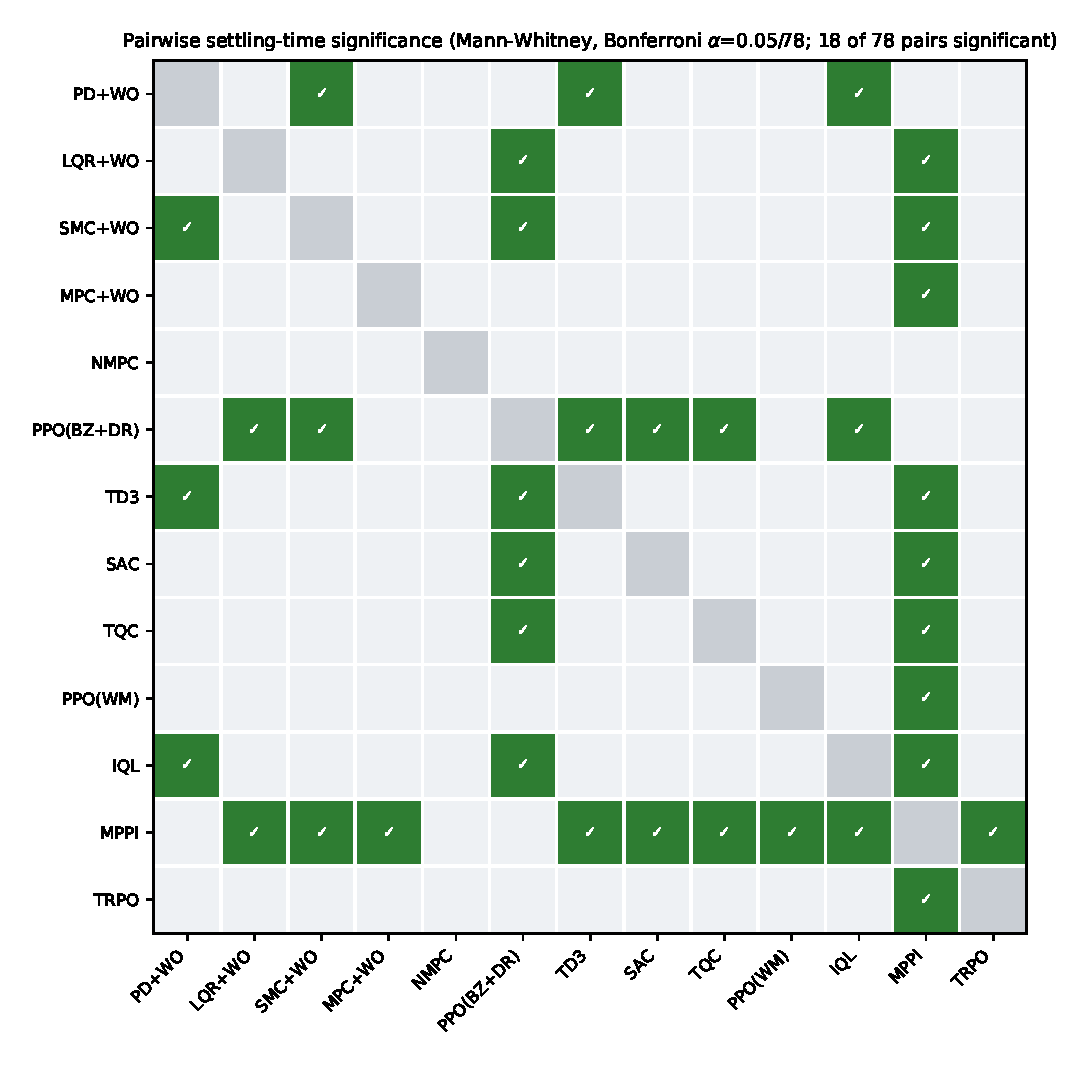
\includegraphics[width=0.95\columnwidth]{figures/exp1_significance_heatmap.eps}
  \caption{Pairwise settling-time significance for the 13 benchmarked
    controllers (Mann-Whitney $U$ rank test on successful trials, Bonferroni
    correction $\alpha = 0.05/78$; 18 of 78 pairs significant). Green cells
    mark significant differences.}
  \label{fig:significance}
\end{figure}

\subsection{Initial Condition Protocol}

We displace the ball from center with a brief cart ``jolt/shake'', noting
its direction post-hoc from the first sensor reading; the cart is moved
automatically by the evaluation script, with no manual ball placement during
trials. For the two at-wall strata the ball side is targeted, and the realized
cart position and side (read per trial from the recorded initial state) vary
somewhat from the nominal targets, as detailed in
Appendix~\ref{appendix:protocol}.
The five-stratum, 50-trial schedule
(Center, Mid-rail, Near-wall, and the two at-wall strata) is specified in
Appendix~\ref{appendix:protocol}.

\subsection{Control Effort and Trajectory Shape}

The qualitative differences behind these numbers show up in three views. The
control-effort distributions (Fig.~\ref{fig:effort_boxplot}) put MPPI and IQL
at the smooth, low-effort end and TD3 and TQC at the aggressive, high-effort
end, matching their RMS-effort figures in Table~\ref{tab:full_results}.
A per-controller gallery of representative ball-angle recoveries
(Fig.~\ref{fig:multi_traj}, one panel per controller, each showing that
controller's median-settling trial) shows the same contrast in recovery
shape: MPPI and PD+WO settle within a few seconds with little overshoot,
while the other wall-override classical controllers (LQR+WO, SMC+WO, MPC+WO)
and the slower simulation-trained agents (SAC, TQC, TD3) take longer and hunt
more before settling. Because each
panel uses a different representative trial, these are illustrations of
typical recovery shape, not a matched head-to-head comparison. The command profiles (Fig.~\ref{fig:action_profiles}) trace one clean recovery
per controller; once the ball is settled the command drops to a small residual
(last-second action RMS around 0.05--0.23 for these representative trials, well
below the $\pm1$ saturation), so these clean-recovery exemplars settle to a
small residual command.

\begin{figure}[t]
  \centering
  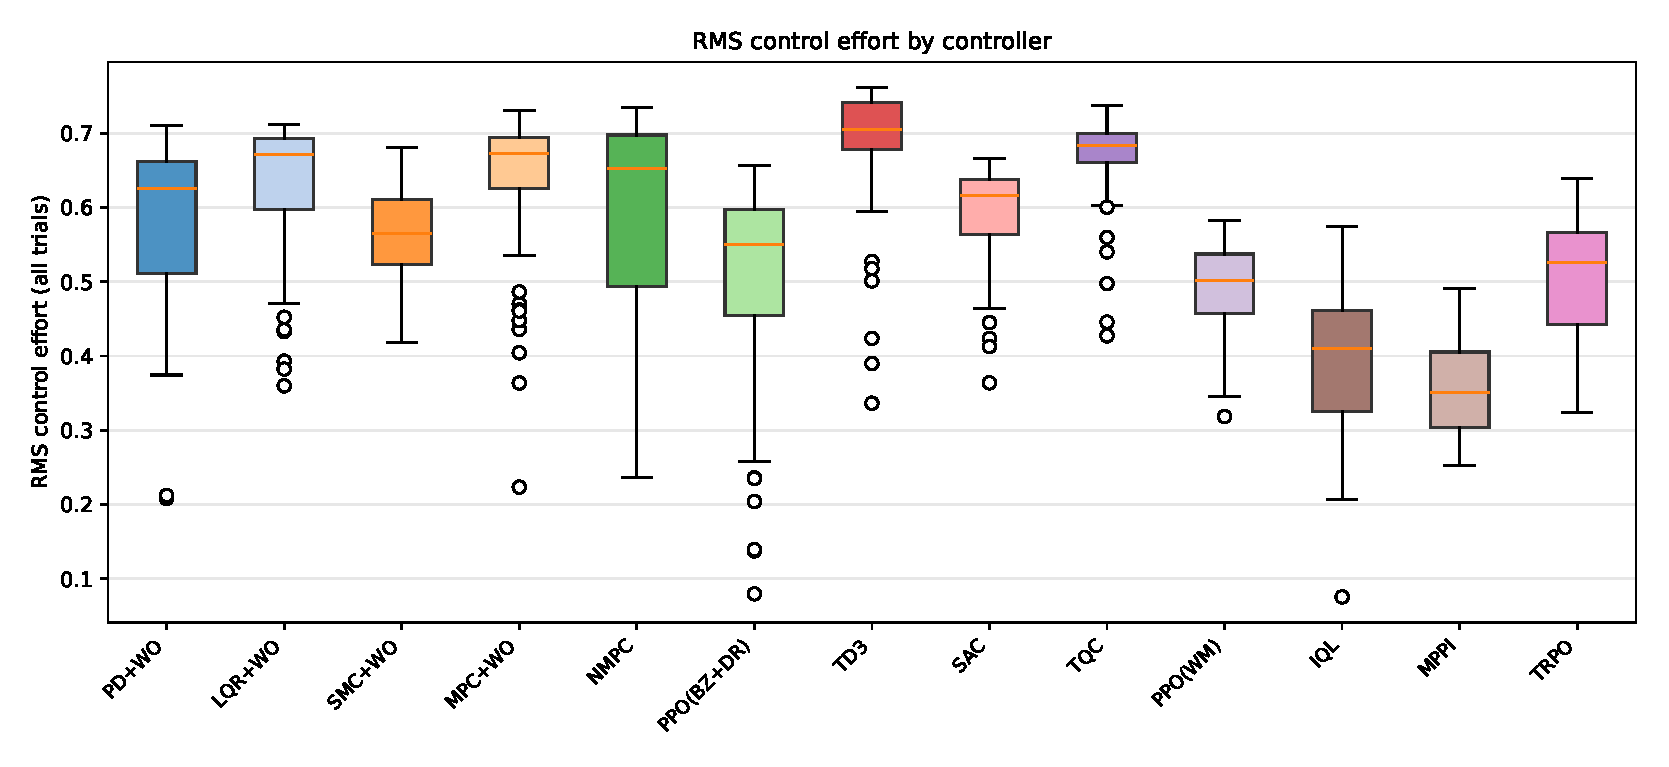
\includegraphics[width=0.95\columnwidth]{figures/effort_boxplot.eps}
  \caption{RMS control effort distribution over all trials.
    MPPI and IQL produce the smoothest, lowest-effort control signals.
    TD3 and TQC show the highest effort, indicating aggressive,
    oscillatory control.}
  \label{fig:effort_boxplot}
\end{figure}

\begin{figure}[t]
  \centering
  
\includegraphics[width=0.95\columnwidth]{figures/compute_time_bars.eps}
  \caption{Mean per-step compute time by controller. MPPI ($\sim$40\,ms)
    runs close to the 50\,ms deadline (red dashed line). IQL, the off-policy
    RL policies (TD3, TQC, SAC), PPO-WM, and NMPC form a second tier at
    2--8\,ms; the classical controllers, MPC, and the on-policy RL policies
    execute in under 1\,ms.}
  \label{fig:compute_time}
\end{figure}

\begin{figure*}[t]
  \centering
  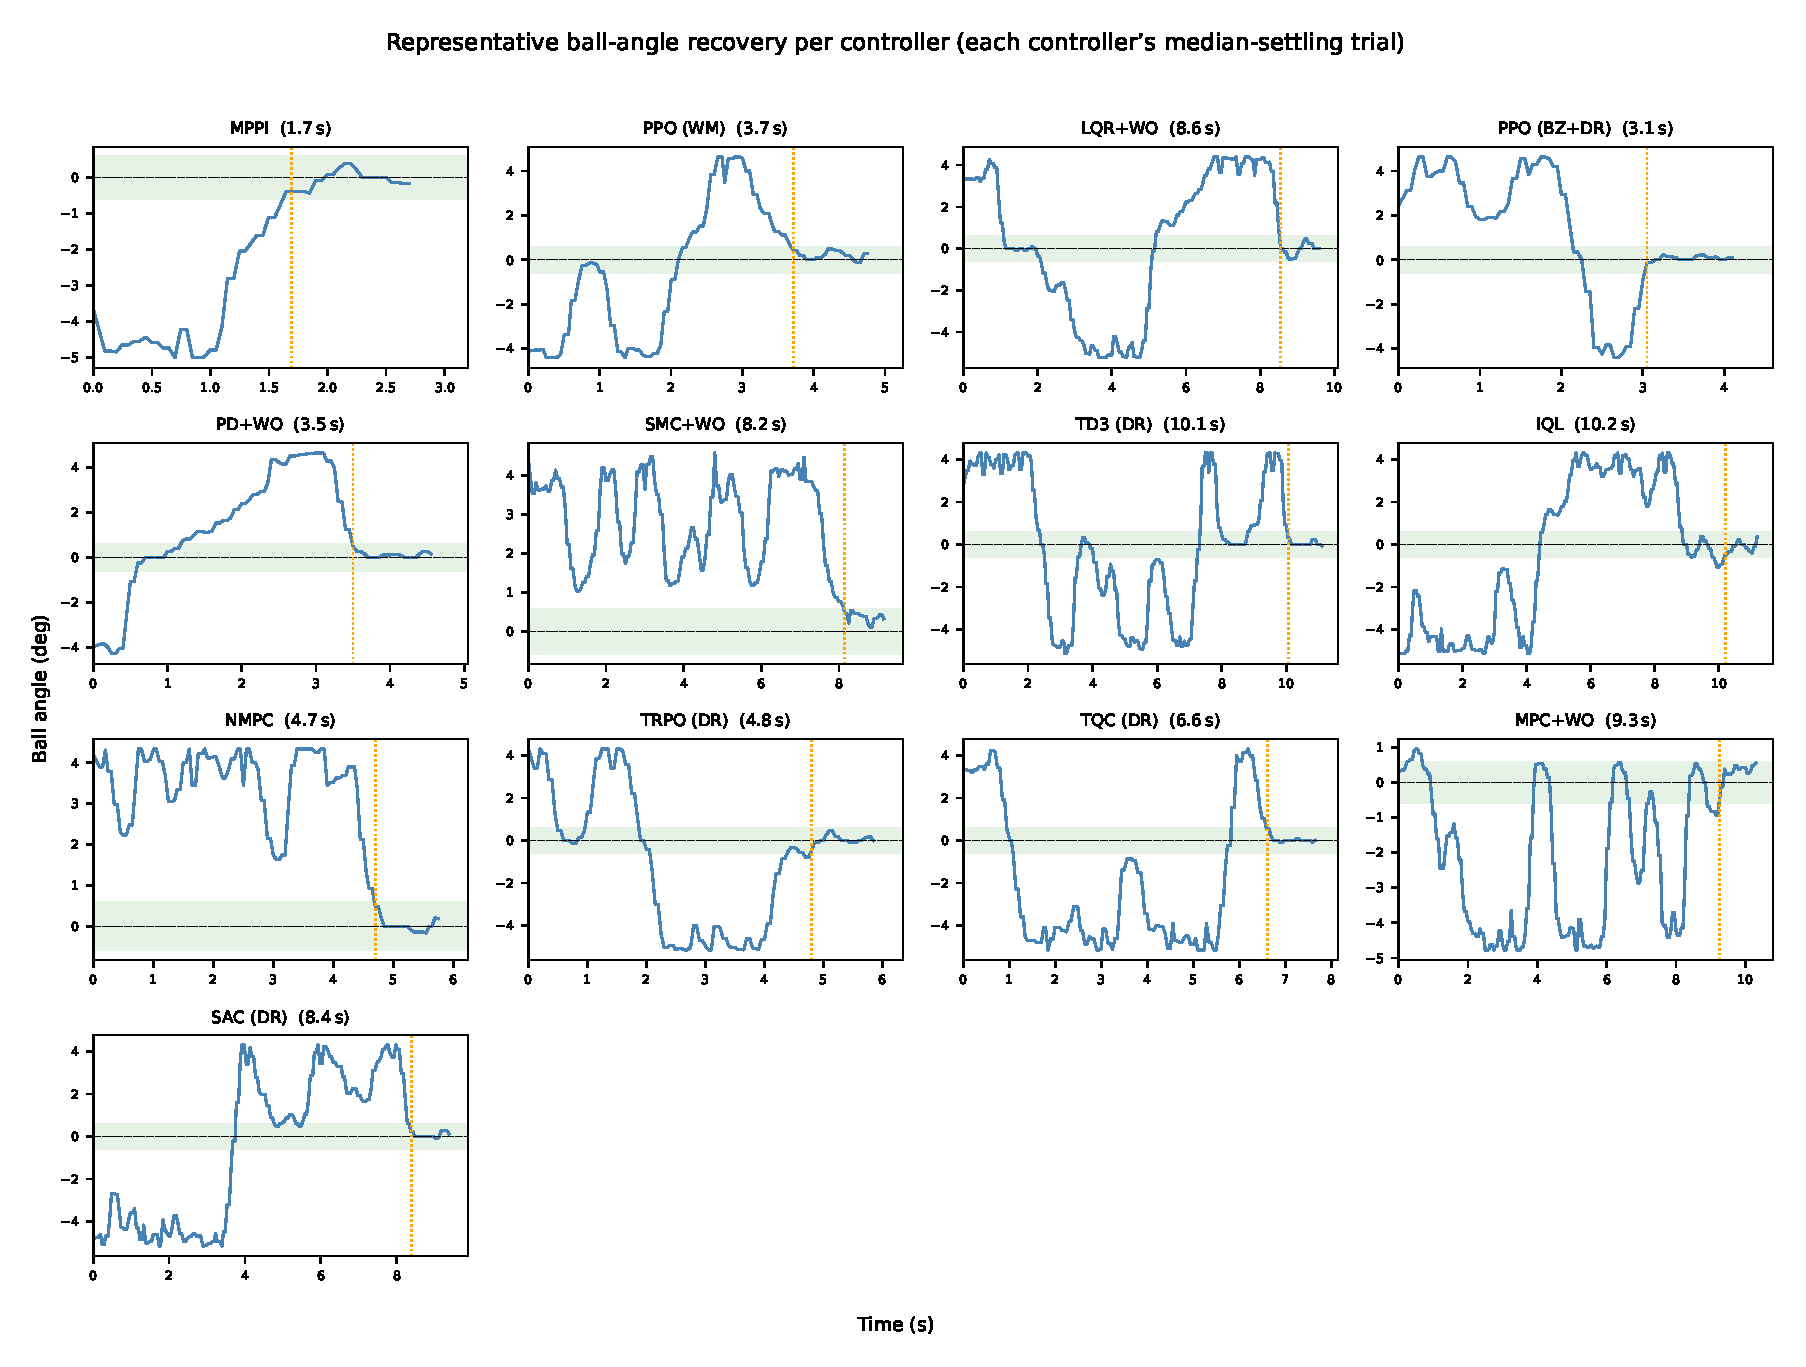
\includegraphics[width=0.95\textwidth]{figures/multi_controller_trajectory.eps}
  \caption{Representative ball-angle recovery for each of the 13 benchmark
    controllers. Each panel shows that controller's successful trial closest
    to its own median settling time (orange dotted line: settling time;
    green band: the $\pm$0.01\,rad settling window). Because each panel uses
    that controller's own representative trial, the initial conditions differ
    across panels, so this is a per-controller view of typical recovery shape
    rather than a matched head-to-head. MPPI and PD+WO recover within a few
    seconds; LQR+WO, SMC+WO, MPC+WO and the slower simulation-trained
    agents (SAC, TQC, TD3) settle later.}
  \label{fig:multi_traj}
\end{figure*}

\begin{figure*}[t]
  \centering
  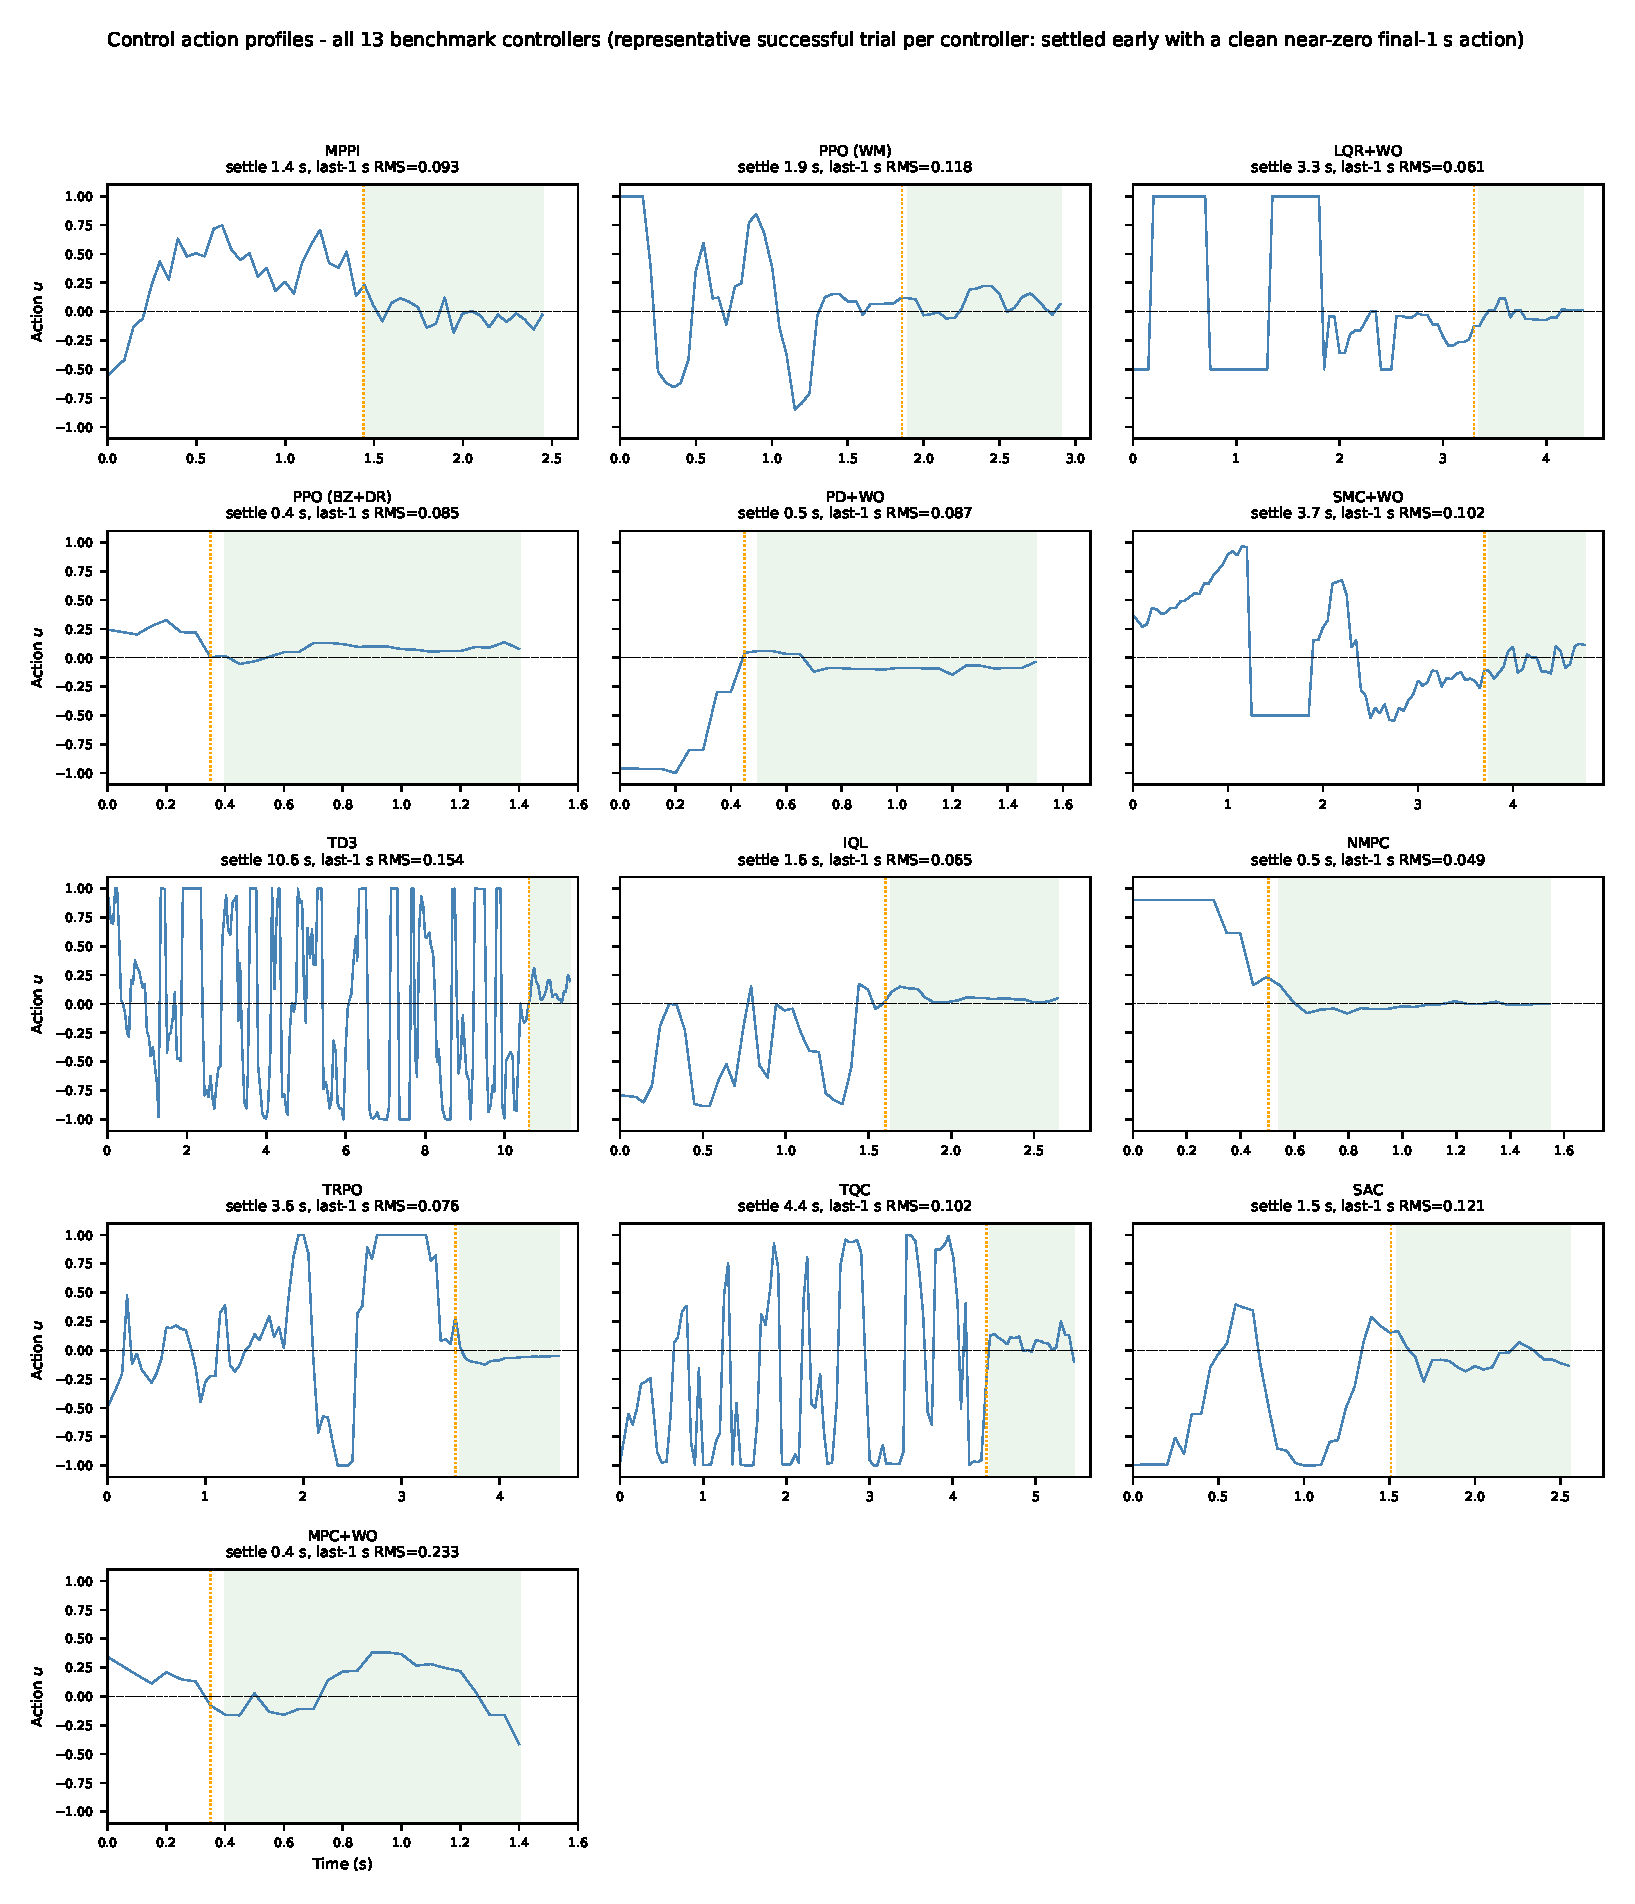
\includegraphics[width=0.95\textwidth]{figures/action_profiles.eps}
  \caption{Control action profiles for all 13 benchmark controllers.
    For each controller the shown trial is selected by a single uniform
    rule: among successful trials that settled reasonably early
    (settling time $\le 1.5\times$ that controller's median) and have at
    least a 1\,s settled tail (episode length $\ge$ settling $+ 1$\,s),
    keep those whose final-1\,s action RMS is within 10\% of that
    controller's best, and pick the earliest-settling of those, i.e.\ a
    clean, early-settling exemplar rather than a barely-settled outlier.
    Shaded green band = the final 1\,s window; orange dotted line = the
    trial's settling time. Last-1\,s action RMS is 0.05--0.23 across
    controllers, i.e.\ commands are near zero once settled. Generated
    from \texttt{paper/data/exp1\_hardware/consolidated.json} by
    \texttt{regenerate\_extra\_figures.py}.}
  \label{fig:action_profiles}
\end{figure*}

\section{Results, Analysis, and Discussion}
\label{appendix:results}

This section presents quantitative results for the experiments described in Appendix~\ref{appendix:protocol}. We emphasize statistical significance, distribution analysis, and practical implications for real-world deployment.



\subsection{Experiment 1: Baseline Performance Results}

Hardware performance was evaluated over 50 trials per controller at 20~Hz
using stratified initial conditions (Section~\ref{sec:ic_design}).
Figure~\ref{fig:hw_ranking} ranks all controllers by success rate;
Figure~\ref{fig:hw_pareto} shows the failure-vs-settling trade-off;
and Figure~\ref{fig:hw_difficulty} decomposes SR by stratum, while
Figure~\ref{fig:settling_by_stratum} does the same for median settling time,
where the pattern is strongly controller-dependent: MPPI stays tight across
strata (1.2--2.7\,s), the wall-override classical controllers mostly slow
toward the boundary (MPC+WO excepted), and the simulation-trained RL agents
swing widely from one stratum to the next, though with only five trials in
each at-wall stratum much of that swing is sampling noise.

\paragraph{Evaluation protocol.}
Every controller in the benchmark received the full 50-trial stratified
evaluation: the five model-free RL algorithms (PPO with BZ+DR; TD3, TQC,
SAC, TRPO with DR), the model-based controllers (MPPI, PPO~(WM)), offline
RL (IQL), and all classical controllers.


\begin{figure}[b]
  \centering
  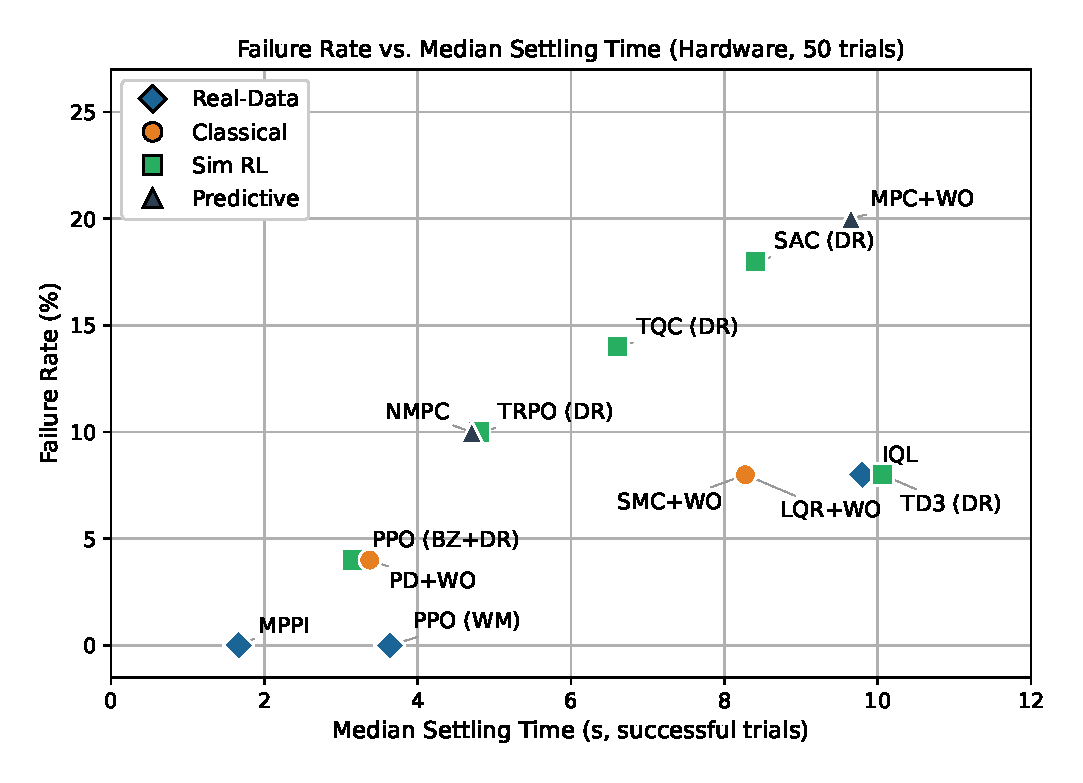
\includegraphics[width=0.95\columnwidth]{figures/hw_sr_vs_settling.eps}
  \caption{Hardware failure rate vs.\ median settling time
    (successful trials); both axes increase toward worse outcomes, so
    the ideal controller occupies the bottom-left corner. MPPI ties for the
    best success rate (100\%, with PPO~(WM)) and has the fastest median
    settling (1.67~s); PPO~(BZ+DR) offers 96\% SR with 3.15~s median settling.}
  \label{fig:hw_pareto}
\end{figure}

\begin{figure}[b]
  \centering
  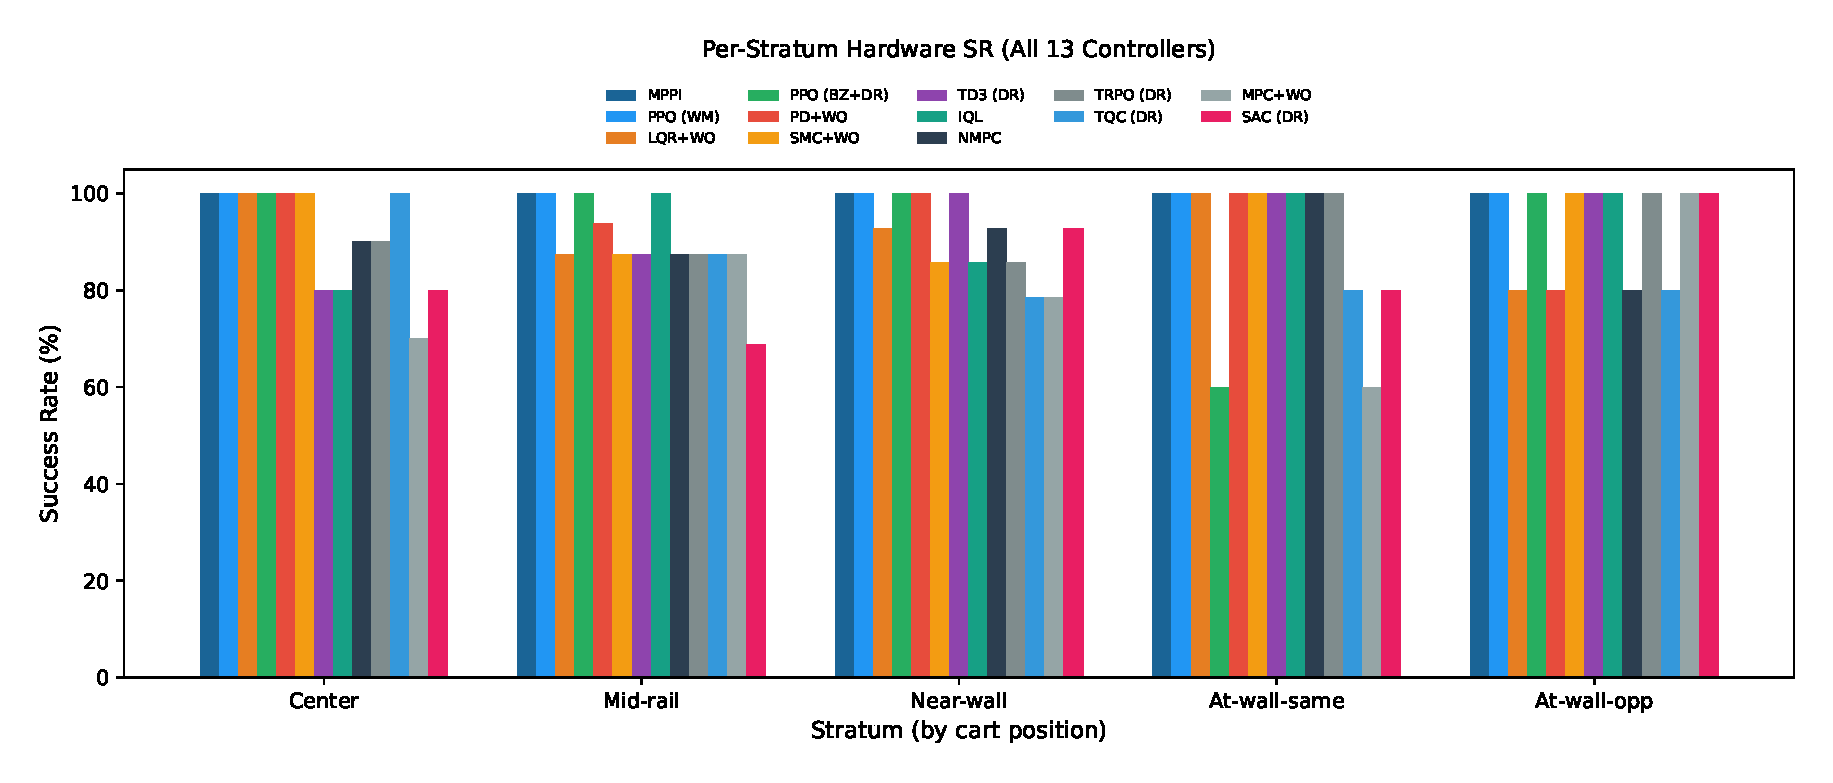
\includegraphics[width=0.95\columnwidth]{figures/settling_by_stratum.eps}
  \caption{Per-stratum hardware SR for all 13 controllers (50 stratified trials).
    Strata are defined mainly by cart starting position; the two at-wall
    strata additionally fix the ball side (Appendix~\ref{appendix:protocol}).
    MPPI and PPO-WM achieve 100\% across all strata;
    aggregate success is in fact lowest on the mid-rail starts
    (about 90\%) and highest on at-wall-opposite (94\%).}
  \label{fig:hw_difficulty}
\end{figure}

\begin{figure}[b]
  \centering
  
\includegraphics[width=0.95\columnwidth]{figures/hw_difficulty_breakdown.eps}
  \caption{Median settling time per stratum for all 13 controllers (successful trials only).
    The slowest stratum is controller-dependent (near-wall or at-wall-same for most),
    while at-wall-opposite is often the quickest, since a ball displaced away from the
    wall gives the controller room to recover; MPPI stays fast across all strata.}
  \label{fig:settling_by_stratum}
\end{figure}

The complete benchmark results table is in Appendix~\ref{appendix:per_trial}
(Table~\ref{tab:full_results}). The analysis below discusses key patterns.

\subsubsection{Simulation Prediction Accuracy}

Appendix~\ref{appendix:simulation_validation} validates the open-loop
prediction accuracy of both the analytical first-principles model and the
LSTM world model against a held-out partition of the 1\,M-transition
hardware dataset.  The world model consistently achieves lower
total-trajectory prediction error (25--35\% lower, across horizons from
0.25--30\,s, with no crossover where the analytical model catches up;
Fig.~\ref{fig:sim_val_crossover}), while on terminal per-channel error the
two are mixed and terminal ball-angle error in particular favors the
analytical model (Table~\ref{tab:sim_val_comparison}).
Nevertheless, the analytical model is sufficient for
classical, predictive, and domain-randomized RL controllers: its
short-horizon error ($<$0.02\,rad ball angle at 0.25\,s) is modest
relative to the ball-angle operating range, and the hardware success rates in
Table~\ref{tab:full_results} show that every controller paradigm
transfers to the real system, though with a residual gap (hardware
success 80--100\%).

\subsubsection{Performance Variability}

Figure~\ref{fig:settling_boxplot} shows the settling-time distributions in
simulation for all thirteen benchmark controllers, each evaluated in the
first-order physics simulator under the identical 50-trial stratified protocol
(seed~42). NMPC is the fastest, with a median near 0.3\,s, yet it takes
4.7\,s on hardware, a compact illustration of the sim-to-real gap; the
simulation-trained RL agents also settle quickly (medians 0.4--2.2\,s), with
TRPO the slowest of them. Notably, the three real-data methods --- MPPI and
PPO~(WM), which plan through or are trained inside the learned world model, and
IQL, trained offline on hardware logs --- also transfer cleanly to the
analytical simulator, each reaching 96--100\% success with median settling
under 0.9\,s, even though none was tuned for the first-order model.

\begin{figure}[!tbp]
  \centering
  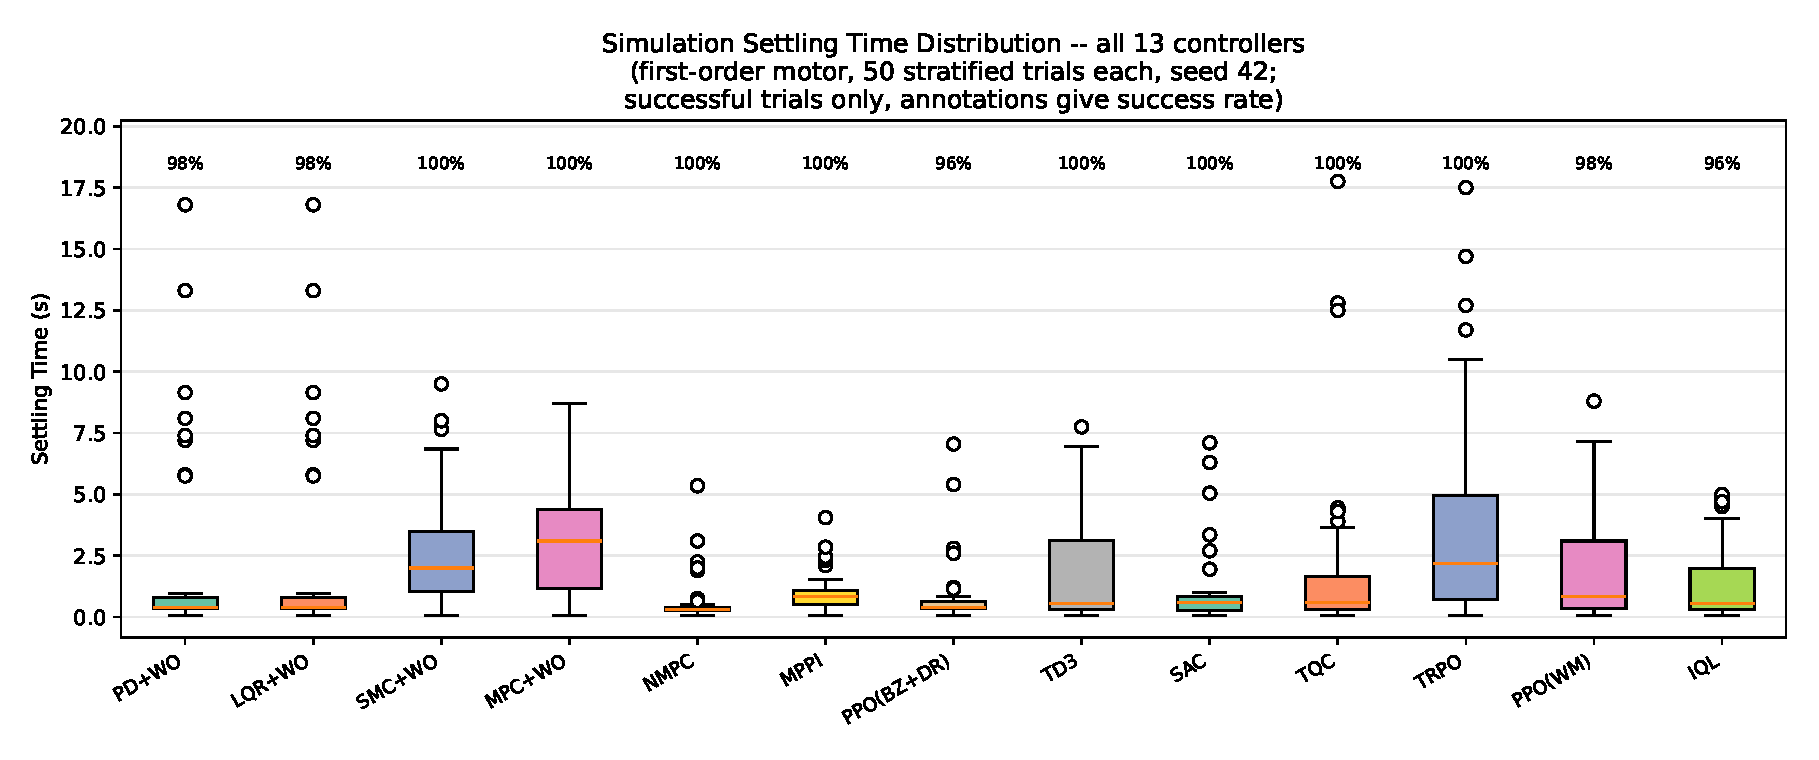
\includegraphics[width=\columnwidth]{figures/settling_time_boxplot_sim.eps}
  \caption{Settling-time distributions in simulation (first-order motor,
    50 stratified ICs, 20~Hz, seed~42; successful trials only) for all
    thirteen benchmark controllers, with success rate annotated above each
    box. NMPC has the fastest median; most controllers settle at medians below
    2.2\,s. The three real-data methods (MPPI, PPO~(WM), IQL) are included for
    completeness: although they plan through or are trained on data rather than
    the analytical model, they still transfer to the physics simulator at
    96--100\% success.}
  \label{fig:settling_boxplot}
\end{figure}

\subsubsection{Initial Condition Robustness}

Figure~\ref{fig:hw_difficulty} decomposes each controller's
hardware success rate across the five cart-position strata (center,
mid-rail, near-wall, and the two at-wall strata). The two at-wall strata
share the same cart target, the physical rail limit, and differ only by
the ball's offset side: \emph{same-side} (ball displaced toward that wall)
and \emph{opposite-side} (ball displaced toward center).

On hardware these initial conditions are realized only approximately: the
cart and ball are reset by hand before each trial, so the achieved cart
position within a labeled stratum varies from trial to trial and between
controllers. We therefore report the per-stratum rates at the
labeled-stratum level and do not attribute per-controller differences to
the exact realized start.

\paragraph{Same-side initial conditions.}
Same-side initial conditions place the ball displaced toward the nearest
wall, which requires the controller to first \emph{reverse} the cart away
from the wall before stabilizing. On hardware, NMPC clears all five
same-side trials (100\%) while MPC+WO clears three of five (60\%).

\paragraph{Classical controllers.}
The design and tuning behind the classical results, and the failure modes
of the variants without constraint handling, are detailed in
Appendix~\ref{appendix:tuning_insights}; here we summarize what the benchmark
shows. With the wall override, LQR reaches 92\% hardware SR by separating
ball regulation (a PD-equivalent gain, since the optimal-control solution
itself fails on hardware) from constraint satisfaction (the
override); its paradigm-native alternative of Q-weighting on cart position is
structurally insufficient, leaving the forced Q-center variant
($K_x = 3.31$) at 28\% and basic LQR at 20\%, the latter failing in every
stratum (40 of 50 trials, including 7 of 10 center and 11 of 14 near-wall
starts) as the
nominal feedback runs out of rail at the limits. SMC with the override reaches 92\% (46/50), up from the basic
variant's 12\%. Two SMC results are specific to hardware. First, sensor-offset
correction is essential: without it SMC+WO falls to 40\%, a 52\,pp drop, far
larger than PD+WO's 8\,pp, because SMC's model-inversion term turns a constant
sensor bias into a persistent spurious velocity command that PD never
generates. Second, its residual 8\% failures (4/50) occur when a blind-zone
limit cycle and a wall approach coincide, the blind zone corrupting the model
inversion into erratic commands that drive the cart toward the rail faster
than the override can clear it. At 8.93\,s mean settling (median 8.28\,s) SMC
is competitive with the other wall-aware classical controllers. PD tells the
same story more simply: the override lifts it from 18\% (vanilla) to 96\% with
calibration (88\% without offset correction), and without the override it
fails every near-wall and at-wall-same trial, with only 2 of 5
at-wall-opposite starts succeeding. When vanilla PD does settle it is
fast (median 1.75\,s versus 3.38\,s for PD+WO, which pays a conservative
retreat), but that speed is moot against its 82\% failure rate. With the
simulator's dip width set to the hardware-measured FWHM, PD+WO reaches 98\% in
simulation against 96\% on hardware, so the two agree on reliability to within a
single trial; settling is faster in simulation (2.15\,s versus 5.80\,s), as
expected without the hardware's sensing and actuation lag. The one extra
hardware failure is consistent with effects the simulator omits, such as the
sensor blind zone ($|\theta| > 0.071$\,rad) and the uncontrolled initial ball
velocity.

\paragraph{Predictive controllers.}
Linear MPC with the wall override reaches 80\% over 50 trials; the basic
QP-constrained variant manages only 44\%, because QP infeasibility near the
walls returns $u=0$ and lets the ball escape (Appendix~\ref{appendix:tuning_insights}).
All 10 MPC failures share the wall-bounce limit cycle described below for
NMPC: the cart sweeps the full track repeatedly (14--23 wall hits per trial)
with the actuator saturated roughly 40--52\% of the time, and the failing trials'
$|\theta_0|$ (mean 0.059\,rad) is indistinguishable from the successes'
(0.060\,rad), so the trap is dynamic rather than a starting-angle threshold.
MPC also reaches only 60\% on same-side starts versus NMPC's 100\%, though
as noted these labeled at-wall starts were realized at differing cart
positions across the two controllers. When it does settle MPC is slower than NMPC (10.81 versus
7.48\,s), and, as with NMPC, center starts are harder than near-wall ones
(70\% versus 79\%) because there is no wall to use as a momentum backstop.

NMPC ($N{=}10$, no wall override) reaches 90\%, the best of the analytical
controllers without an external wall override, by planning
constraint-satisfying trajectories through its
nonlinear model~\cite{mayne2014mpc}. Its 5 failures share one mechanism,
independent of stratum (1 center, 2 mid-rail, 1 near-wall, 1
at-wall-opposite): a wall-bounce limit cycle rooted in a mismatch between the
planner's wall model and what the cart physically does at the rail. We
verified the causal chain across all 50-plus wall hits in the failed trials.
NMPC does plan to brake in time, at every recorded hit the commanded action
already pointed away from the wall, but the 0.5\,s horizon (10 steps) cannot
arrest the momentum built during a full cross-track rescue, so the cart
reaches the rail with 0.26--0.59\,m/s of residual velocity. The NLP encodes
the rail only as a hard bound on cart position, not as a model of the rebound,
so when the cart hits the rail its velocity reverses in a way the internal
model never anticipates. The warm-start, which assumed the cart would taper to
rest at the boundary, now carries the wrong sign on the most safety-critical
state, and IPOPT settles into a local minimum: because the opposite-wall
rescue also minimizes ball-angle error within the 0.5\,s window, the solver
commits to it and drives the system toward the next rebound a second or two
later, outside the horizon. The cycle then locks in, 44--51\% of steps
saturate the actuator ($|u|{>}0.85$), the cart sweeps $\pm$0.78\,m repeatedly,
and $\theta$ oscillates near $\pm$0.08\,rad; the one-second settling window is
never met (Trial~14 reached 20 consecutive in-band steps at $t{=}10.1$\,s
before the next rebound reset the count). The failing trials' $|\theta_0|$
(0.066\,rad) again matches the successes' (0.062\,rad), and all five
at-wall-same trials succeed, though only some were realized at the rail, so
this stratum does not by itself establish immunity to the rebound. Two further points, detailed
in Appendix~\ref{appendix:tuning_insights}: the short horizon is essential (at
$N{=}30$, stale observations let NMPC pass only 1 of 7 tuning initial
conditions on hardware), and its internal dip width of
42\,mm, against the true 20\,mm, is beneficially conservative, giving smoother
recoveries. NMPC reaches 100\% on at-wall-same starts, matched there by LQR+WO.

\paragraph{Real-data and learning-based controllers.}
MPPI gives the best overall result, 100\% SR at 2.06\,s mean settling, the
fastest of the reliable controllers, using sampling-based MPC over the learned LSTM
world model. PPO~(BZ+DR) reaches 96\% SR (3.81\,s mean settling); blind-zone
modeling and domain randomization together are what make its sim-to-real
transfer work. Among the
other simulation-trained agents, TD3~(DR) reaches 92\% but with the slowest
settling (11.45\,s), its deterministic policy gradient~\cite{fujimoto2018td3}
giving consistent responses, and TQC~(DR) 86\% at 9.77\,s from its
distributional critics~\cite{kuznetsov2020controlling}. The two training
ingredients contribute measurably: domain randomization~\cite{tobin2017domain}
adds 30\,pp to PPO's hardware SR (60\% to 90\%), and the blind-zone model a
further 8\,pp (90\% to 98\%), confirming that modeling the VL53L0X
minimum-range saturation matters for deployment. These ablations are
measured in the S-curve training family; the policy reported in
Table~\ref{tab:full_results} is the matched first-order-lag checkpoint at
96\% (Appendix~\ref{appendix:rl_fairness}). PPO~(WM), trained entirely
inside the learned world model with no domain randomization
(Appendix~\ref{appendix:world_model}), also reaches 100\% across all
50 trials (joining MPPI); its mean settling (6.84\,s) is inflated by a few high outliers but
its median (3.64\,s) is competitive. IQL reaches 92\% from purely offline
training on roughly 333k real post-recalibration transitions with no
simulator, placing it mid-table among the deployed controllers; its mean
and median settling (10.62 and 9.80\,s) are close to TQC's, but it has the
lowest control effort of any RL controller (0.395), reflecting the
conservatism of implicit Q-learning. Its failures fall on center starts
(2/10) and near-wall starts (2/14), while every at-wall trial succeeds
(10/10). The most control-efficient
controllers are the learned and real-data ones: MPPI's RMS effort (0.354) is
the lowest of the deployed set, followed by IQL (0.395), PPO~(WM) (0.492), and
PPO~(BZ+DR) (0.498), all well below NMPC (0.608) and LQR+WO (0.625). The
off-policy agents are the exception, with TD3 (0.680) and TQC (0.663) among
the highest.

Pairwise testing confirms this ordering is not noise, and control effort is the
axis on which the benchmark most clearly separates controllers: 58 of the 78
RMS-effort comparisons are significant (Mann-Whitney, Bonferroni corrected as a
separate family), against 18 of 78 for settling and 0 of 78 for success rate.
MPPI and IQL each use significantly less effort than every other controller
except one another, with which they are statistically tied. PPO~(WM) sits
mid-range, significantly gentler than the classical, MPC, and off-policy
controllers but not separable from PPO~(BZ+DR) or TRPO, consistent with the
weak action response of its world model (Appendix~\ref{appendix:world_model}).
The full pairwise matrix is written to \texttt{exp1\_effort\_significance.csv}.

\section{Real-Hardware Fine-Tuning}
\label{appendix:finetuning}

\subsection{Motivation}

Despite domain randomization and sensor modeling reducing the
sim-to-real settling-time gap to $3.0\times$
(Appendix~\ref{appendix:sim2real}), the question remains whether
online fine-tuning on real hardware can further close this gap.
We fine-tune three deployed policies on real hardware: the two best
sim-trained agents, one on-policy (PPO~(BZ+DR)) and one off-policy (TD3),
and the world-model policy PPO~(WM), to compare adaptation strategies.

\subsection{Protocol}

We fine-tune all three policies directly on the real system in the
\texttt{BalancerReal} Gym environment, with an
augmented reward signal:
\begin{equation}
  r_t^{\text{FT}} = \mathrm{clip}\bigl(r_t^{\text{balanced}} + d_t,\; -1,\; 1\bigr)
\end{equation}
where $d_t \in \{0, 1\}$ is the binary infrared dip-sensor signal
(1 while the ball physically obstructs the beam at the arc's lowest
point, 0 otherwise). The beam is broken over an active band narrower
than the ball diameter, so $d_t$ fires only within a few millimeters of
true center; this is the raw hardware bit, not the wider offline angular
proxy ($\theta_\text{center} = 0.007$\,rad) that
Appendix~\ref{appendix:dataset_details} uses when rebuilding the logged
dataset. It provides a strong, noise-free reward signal at the exact
balancing target that is unavailable in simulation.
The environment does not terminate on cart or ball limits; only the 30\,s
\texttt{TimeLimit} truncates an episode, and the per-step reward is the
clipped balanced-plus-dip signal above, not overwritten at the limit.

Table~\ref{tab:ft_protocol} lists the fine-tuning hyperparameters.
All three policies use a reduced learning rate ($10^{-4}$, vs.\ $3\times10^{-4}$
for PPO and $10^{-3}$ for TD3 during sim training) to prevent
catastrophic forgetting.

\begin{table}[!t]
\centering
\renewcommand{\arraystretch}{1.15}
\caption{Fine-tuning protocol. The PPO~(BZ+DR) base model is the S-curve
  development policy (98\% hardware SR); Table~II (main paper) reports the
  matched first-order-lag checkpoint at 96\% (Appendix~\ref{appendix:rl_fairness}).}
\label{tab:ft_protocol}
\begin{tabular}{lcc}
\toprule
\textbf{Parameter} & \textbf{PPO FT} & \textbf{TD3 FT} \\
\midrule
Base model           & PPO (BZ+DR)           & TD3 (DR)              \\
Learning rate        & $10^{-4}$             & $10^{-4}$             \\
Total steps          & 50\,000               & 50\,000               \\
Wall-clock time      & $\sim$50\,min         & $\sim$50\,min         \\
Episodes             & $\sim$83              & $\sim$83              \\
Checkpoint freq      & 5\,000 steps          & 5\,000 steps          \\
Reward               & balanced + IR dip     & balanced + IR dip     \\
Entropy coeff        & 0.005                 & --                   \\
\bottomrule
\end{tabular}
\end{table}

\subsection{Results}

Table~\ref{tab:ft_results} compares pre-FT and post-FT hardware
performance, and Fig.~\ref{fig:finetuning_results} shows it graphically: the
PPO~(WM) settling-time distributions before and after fine-tuning differ
modestly (both 100\% SR), alongside the success-rate comparison
for all three fine-tuned models.

\begin{table}[!t]
\centering
\renewcommand{\arraystretch}{1.15}
\caption{Fine-tuning results: hardware evaluation.
         PPO~(WM) evaluated on 50 stratified trials;
         PPO~(BZ+DR) and TD3 on 10 trials each.}
\label{tab:ft_results}
\begin{tabular}{lccccc}
\toprule
\textbf{Model} & \textbf{N} & \textbf{SR} & \textbf{Mean (s)}
  & \textbf{Med (s)} & \textbf{Max (s)} \\
\midrule
\multicolumn{6}{l}{\textit{Pre-fine-tuning:}} \\
PPO (WM)           & 50  & 100\% & 6.84 & 3.64 & --  \\
PPO (BZ+DR)        & 10  & 100\% & 4.98 & --  & 13.66 \\
TD3 (DR)           & 10  & 100\% & 8.16 & --  & 23.00 \\
\midrule
\multicolumn{6}{l}{\textit{Post-fine-tuning:}} \\
PPO (WM) + FT      & 50  & 100\% & 7.03 & 5.41 & --  \\
PPO (BZ+DR) + FT   & 10  &  90\% & 6.50 & 4.66 & 21.71 \\
TD3 (DR) + FT      & 10  &  80\% & 8.60 & 5.85 & 26.65 \\
\bottomrule
\end{tabular}
\end{table}

\begin{figure}[!t]
  \centering
  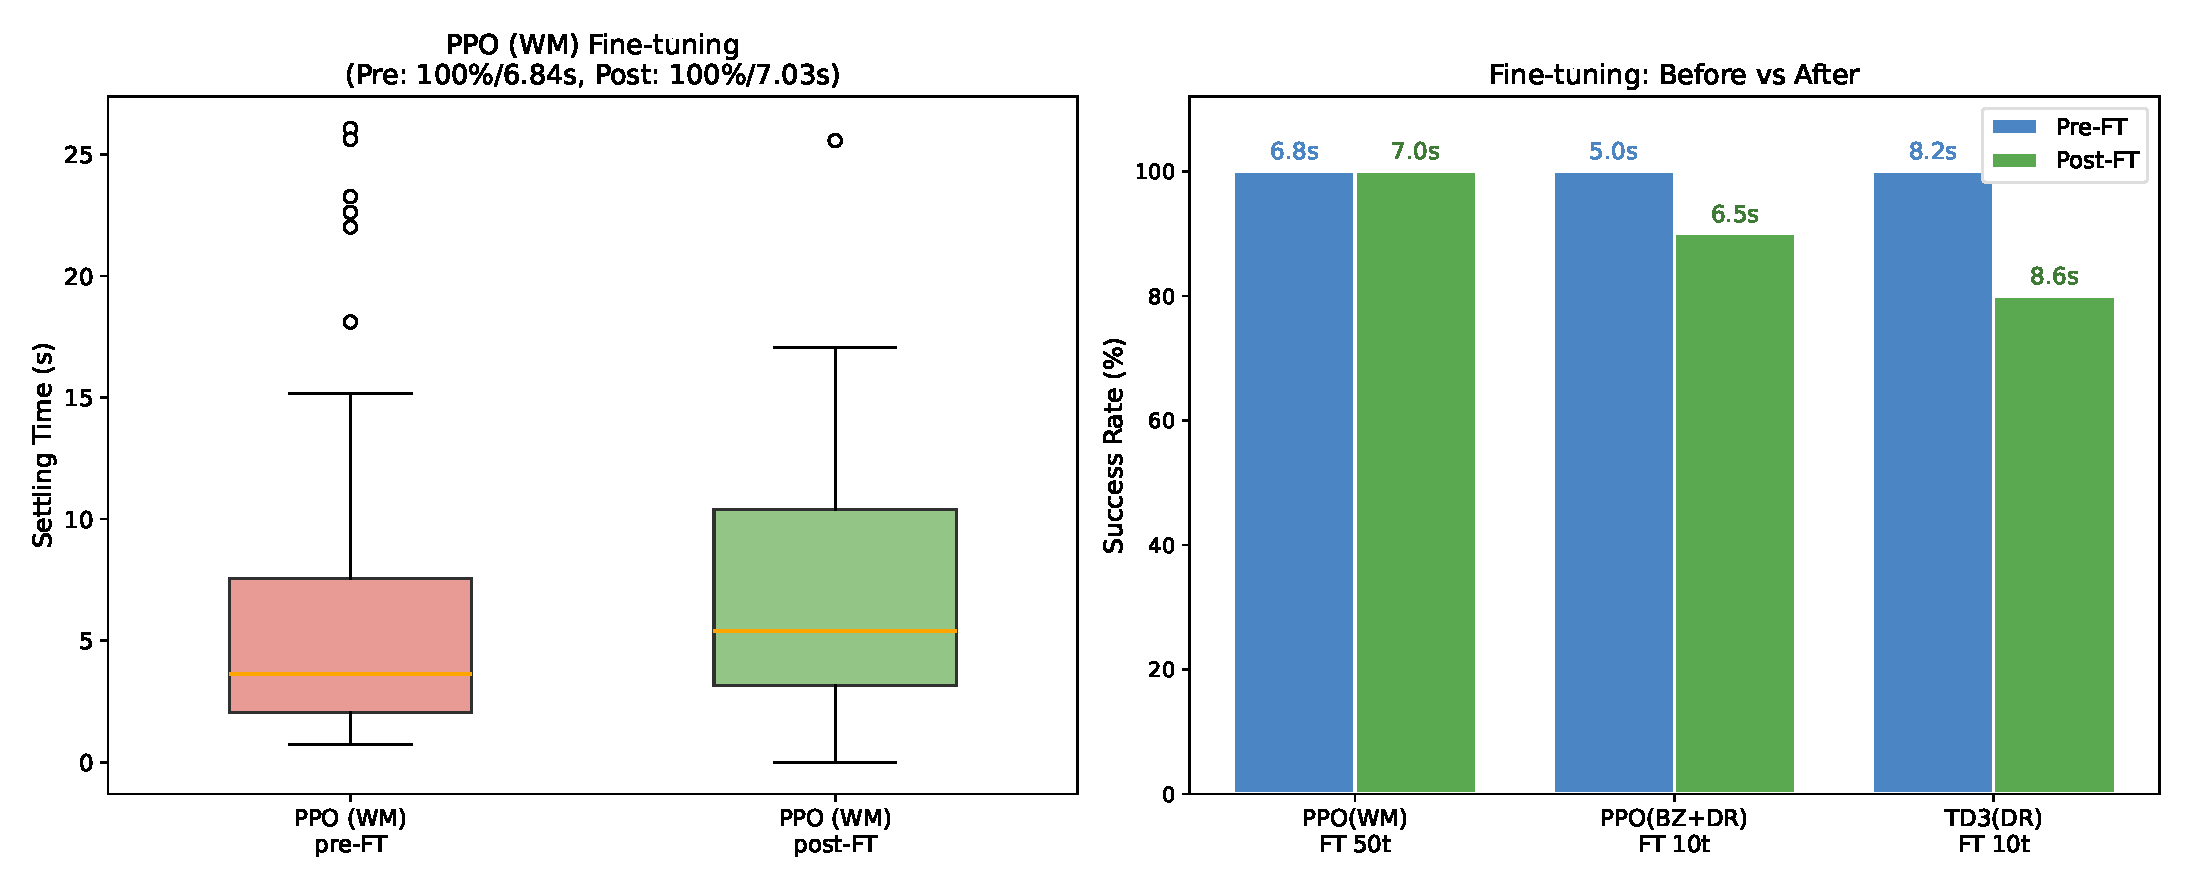
\includegraphics[width=\columnwidth]{figures/finetuning_results.eps}
  \caption{Fine-tuning comparison. Left: PPO~(WM) settling time
    distribution before and after fine-tuning (50 trials each, both 100\% SR).
    Right: success rate comparison for all fine-tuned models with
    mean settling time annotations.}
  \label{fig:finetuning_results}
\end{figure}

\subsection{Analysis}

\paragraph{PPO~(WM) fine-tuning.}
The world-model PPO, fine-tuned for 50K steps on real hardware,
retains 100\% SR, and the before/after settling-time distributions differ
in shape (a higher post-fine-tuning median, 3.64\,s~$\to$~5.41\,s, and a
heavier upper tail), but not significantly (Mann-Whitney on settling
times, $p = 0.27$); the means stay close (6.84\,s~$\to$~7.03\,s).
The mean episode reward dips at the onset of fine-tuning and then recovers
slowly over the 50K steps, ending near its starting level, so the fine-tuning
step itself is not failing; the policy changes only modestly under real-data
gradients on this budget. On this 50-trial evaluation, online adaptation did
not produce a measurable improvement, consistent with the world-model policy
already capturing much of the relevant dynamics.

\paragraph{Sim-trained model fine-tuning.}
On a matched 10-trial hardware evaluation, fine-tuning did not improve either
policy and moved each by one or two of ten trials: PPO~(BZ+DR) from 10/10 to
9/10 and TD3 from 10/10 to 8/10, both with slightly longer settling. These 10-trial
figures sit against the 50-trial baselines of 98\% (PPO~(BZ+DR))
and 92\% (TD3), so the effect is small in absolute terms; at 10 trials these
one- and two-trial changes are within sampling noise, and we observe no
improvement from fine-tuning on either paradigm at this budget.

\paragraph{Root causes.}
Three factors plausibly contribute. The first is simply too little data: 50k
steps is roughly 83 episodes per policy (30\,s trials at 20\,Hz), against the
3M (PPO) and 1M (TD3) steps of the original simulation training, far too little
real experience to learn a meaningful improvement. The second is catastrophic
forgetting: even at the reduced learning rate ($10^{-4}$), gradient updates
from a handful of real episodes partly overwrite the simulation-trained
policy, and the low-reward episodes from at-wall starts corrupt the value
function. The third is that the pre-fine-tuning models are already near their
ceiling: PPO~(BZ+DR) reaches 98\% over 50 hardware trials without any
fine-tuning, and its single failure, on a center start, may need an
architectural change rather than more data to close.

\paragraph{On-policy vs.\ off-policy.}
PPO changed by one of ten trials and TD3 by two; at this sample size the
difference between them is not meaningful, and neither improved with this
budget.

\paragraph{Implications.}
These results validate the sim-to-real approach taken in this work:
careful simulation modeling produces policies that transfer effectively
without online adaptation, and PPO~(BZ+DR) already sits near the
reliability ceiling on hardware. On this budget online fine-tuning does
not help: as the reward curve shows, the policy first unlearns and then
relearns, spending the real interaction returning to where it started
rather than improving. Because the deployed policy is already
near-ceiling and a learned world model already captures the system's
dynamics well (its prediction accuracy plateaus by roughly 100k
transitions, Appendix~\ref{appendix:world_model}), training PPO inside
that world model (PPO-WM) or relying on one-shot transfer is a more
effective use of effort than online fine-tuning on the physical rig.

Future work could investigate:
\begin{itemize}
  \item Longer fine-tuning budgets ($>$500K real steps,
    $\sim$8 hours of continuous operation).
  \item Replay buffer seeding with sim data (for TD3/SAC)
    to prevent catastrophic forgetting.
  \item Residual policy learning: training a small correction
    network on top of the frozen sim policy.
  \item System identification: using real trajectories to
    update the simulation model rather than the policy directly.
\end{itemize}


% ------------------------------------------------------------
% PART V - Reproducibility
% ------------------------------------------------------------
\section{Reproducibility Guide}
\label{appendix:reproducibility}

All code, trained models, datasets, and evaluation scripts are available at
\url{https://github.com/JDRanpariya/ball-balancing-on-arc}, together with
per-subdirectory READMEs that give exact run instructions. This appendix
only summarizes what is where; please refer to the repository for commands.

\subsection{Hardware}

Table~\ref{tab:hw_components} lists the physical components of the
ball-on-arc platform.

\begin{table}[H]
\centering
\caption{Hardware components.}
\label{tab:hw_components}
\begin{tabular}{lp{5.2cm}}
\toprule
\textbf{Component} & \textbf{Specification} \\
\midrule
3D-printed cart & PLA; its top surface is the convex arc ($R = 2.101$\,m, $\approx$30\,cm span) with a shallow central dip (2\,mm deep, 20\,mm FWHM); rides the actuator carriage \\
Ball & Steel, $m = 24$\,g, $r = 9$\,mm \\
Linear actuator & SMC LEFB32NXS-1000, 1000\,mm belt-driven stroke~\cite{smc_lefb_catalogue} \\
Servo motor \& drive & Beckhoff AM8121 motor via an EL7201 EtherCAT servo terminal \\
Controller & Beckhoff C6015 IPC, TwinCAT~3 runtime \\
Ball sensors & 2$\times$ VL53L0X ToF~\cite{vl53l0x_datasheet} at the arc edges (read alternately), plus a center IR beam-break, acquired by an Arduino Uno \\
Host PC & Windows (TwinCAT), Python stack in WSL2; USB serial to the drive and Arduino \\
\bottomrule
\end{tabular}
\end{table}

\paragraph{Note on length units.}
The rail provides approximately 1\,m of physical cart travel
(1000\,mm actuator stroke), yet the drive reports positions at roughly
twice that physical displacement, and the soft-limited operating window
spans 1.553\,m in these axis units ($\pm 0.7765$\,m about the center).

The factor comes from the drive's encoder scaling. The released NC
configuration (\texttt{hardware/twincat/axis\_parameters.xml}) sets
\texttt{ScaleFactorNumerator} $= 104.8576$ against
\texttt{ScaleFactorDenominator} $= 1048576$, that is $10^{-4}$ axis
units per encoder increment. With the EL7201 at its default 20
single-turn bits ($2^{20}$ increments per revolution), this amounts to
a feed constant of $104.8576$\,mm per motor revolution, which is the
encoder count rescaled rather than a measured quantity. The belt drive
advances $54$\,mm per revolution (the catalogued equivalent lead of the
LEFB32 AC-servo variant), so reported positions run
$104.8576/54 \approx 1.94$ times the physical ones. On that factor the
operating window is about $0.80$\,m of the $1000$\,mm stroke, leaving
roughly $0.10$\,m of margin at each end, which is what the mechanical
end stops require.

It affects
no result: all positions, velocities, limits, identified dynamics, and
results in the paper and code use these axis units consistently. The
factor matters only when comparing quoted track lengths against the
physical bill of materials.

\subsection{Software}

The reference environment pins Python~3.11, NumPy~2.2.6, SciPy~1.16.0,
PyTorch~\cite{paszke2019pytorch} 2.10.0, Stable-Baselines3~\cite{stable_baselines3} 2.9.0,
sb3-contrib~2.9.0, d3rlpy~\cite{seno2022d3rlpy} 2.8.1 (IQL), CasADi~\cite{casadi} 3.7.2 (NMPC),
and OSQP~\cite{osqp} 1.1.3 (MPC); exact versions are locked in \texttt{env.yaml} and
\texttt{requirements.lock.txt}.

\subsection{Repository layout}

\begin{itemize}
  \item \texttt{balancer/} (core library): all 13 controllers, simulation and hardware environments, and PLC/sensor interfaces.
  \item \texttt{hardware/}: bill of materials and assembly guide, 3D-print STLs, the TwinCAT project, Arduino sensor firmware, and wiring documentation.
  \item \texttt{training/}: RL, offline-RL, and world-model training scripts and configuration files.
  \item \texttt{evaluation/}: benchmark evaluation, controller tuning, and profiling scripts.
  \item \texttt{data/}: datasets and data-driven models (including the 1M random-exploration dataset and the ${>}$1M-transition logged-trial archive).
  \item \texttt{paper/}: paper source and the result data backing every table and figure.
  \item \texttt{scripts/}: repository utilities.
\end{itemize}

\subsection{Sensor calibration (hardware runs only)}

Reproducing figures and tables from the committed data needs no calibration.
For fresh on-hardware campaigns, the two time-of-flight sensors are
recalibrated first, following Stage~4 of the repository reproducibility guide:
the calibration script prints the per-sensor center offsets, which are
written back to \texttt{balancer/balancer/hardware/constants.py} once the two arc
halves report a consistent zero (the deployed datasets use the recalibrated
constants $189$/$158$~mm; the earlier $175$/$170$~mm values and the bias
they left are analyzed in
Appendix~\ref{appendix:sensor_characterization}). The offsets drift slowly, so we recalibrate before each new
data-collection or evaluation campaign.

\subsection{Reproducing the project}

The repository is built to reproduce the whole project end to end, not only
the paper's numbers. The step-by-step guide, \texttt{reproducibility\_guide.md},
with the per-directory READMEs, documents the full pipeline: building and
wiring the platform, deploying the PLC firmware, setting up the pinned
environment, calibrating the sensors, collecting datasets, training the
learning-based controllers, and evaluating all 13 controllers in simulation
and on the rig. The paper's tables and figures, the simulation validation,
and the wall-override ablations are the final stage of that pipeline and
regenerate from the committed data through the documented scripts, with no
hardware required. The master hardware-results file that backs Table~1 and the
hardware figures is itself rebuildable from the per-controller run aggregates
by \texttt{data/build\_consolidated.py}, which also emits the full
source-to-entry provenance manifest and checks that the rebuild is
byte-identical to the committed file. We do not duplicate the commands here.

\subsection{Companion website}

An interactive version of this benchmark, including the browser-based
simulation and per-controller trial videos, is available at
\url{https://ball-on-arc.pages.dev/}. The site carries no author,
affiliation, or institution identifiers.

\subsection{Key Parameters}

Table~\ref{tab:critical_params} collects the experimental parameters
held fixed across every benchmark trial.

\begin{table}[H]
\centering
\caption{Critical experimental parameters.}
\label{tab:critical_params}
\begin{tabular}{ll}
\toprule
\textbf{Parameter} & \textbf{Value} \\
\midrule
Control frequency & 20\,Hz (50\,ms period) \\
Trial duration & 30\,s maximum \\
Settling band & $\pm 0.01$\,rad \\
Settling duration & 1.0\,s continuous \\
Random seed (ICs) & 42 \\
Number of trials & 50 per controller \\
ToF timing budget & 34.5\,ms \\
Action range & $[-0.9, 0.9]$\,m/s (velocity set-point, axis units) \\
Cart limits & $\pm 0.7765$\,m (axis units) \\
\bottomrule
\end{tabular}
\end{table}

\clearpage

\bibliographystyle{IEEEtran}
\bibliography{bibliography}

\end{document}
